% ------------------------------------------
%  MASTER THESIS DISSERTATION
% ------------------------------------------
% Author:
%
% Advisors:
%
% ------------------------------------------
\documentclass[10pt,twoside,openright,a4paper]{report}
\usepackage[utf8]{inputenc}

% Set document margins to 1in in all sides
\usepackage[margin=2.5cm]{geometry}
% Line spacing package
\usepackage{graphicx, helvet, hyperref, setspace}
\usepackage[portuguese,english]{babel}
\usepackage[acronym, toc]{glossaries}
% Extra stuff file
% This file is included before begin{document} environment
% Use this to include extra packages and define your own commands
% This way, you can easily grab a most recent version
% of dissertation.tex file from the original repo
\usepackage{amsmath,amssymb,amsfonts}
\usepackage{algorithmic}
\usepackage{graphicx}
\usepackage{textcomp}
\usepackage{xcolor}
\usepackage{array}
\usepackage{multirow}
\usepackage{arydshln}
\usepackage{algorithm}
\usepackage{algorithmic}
\usepackage{subcaption}
\usepackage{amsmath}%
\usepackage{tikz}%
\usepackage{pgfplots}%
\pgfplotsset{width=7cm,compat=1.7}%
\pgfplotsset{%compat=1.11,
    /pgfplots/ybar legend/.style={
    /pgfplots/legend image code/.code={%
       \draw[##1,/tikz/.cd,yshift=-0.25em]
        (0cm,0cm) rectangle (3pt,0.8em);},
   },
}
\usetikzlibrary{patterns}
%\usepackage{ctable} 
\definecolor{darkgreen}{RGB}{0,166,79}

\usepackage{amsthm}

% Built the glossary when the main file is built.
\makeglossaries
% Set main font to Arial
\renewcommand{\familydefault}{\sfdefault}
% Define keywords macro
\providecommand{\keywords}[1]{\textbf{Keywords:} #1}
% Define the NewPage macro
\newcommand*\NewPage{\newpage\null\thispagestyle{empty}\cleardoublepage}
% Abstract-en page numbering
\newcommand {\abstractEnglishPageNumber} {\thispagestyle{plain}\setcounter{page}{\abstractEnglishPage}}
% Abstract-pt page numbering
\newcommand {\abstractPortuguesePageNumber} {\thispagestyle{plain}\setcounter{page}{\abstractPortuguesePage}}
% Section numbering depth
\setcounter{secnumdepth}{2}
% Table of contents depth
\setcounter{tocdepth}{3}
% Set line spacing to 1.5cm
\onehalfspacing
% Page numbering
\pagestyle{plain}

% Glossary-File
% Glossary Definition

\newglossaryentry{MSc}{name={MSc}, description={Masters degree in the area of Science.}}
% Acronym-File
% Acronym Definition

\newacronym{IST}{IST}{Instituto Superior T\'ecnico}
\newacronym{HRI}{HRI}{Human-Robot Interaction}


\makeatletter
\newtheoremstyle{indentedsty}
  {1em}% space before
  {1em}% space after
  {\addtolength{\@totalleftmargin}{2em}
   \addtolength{\linewidth}{-8em}
   \parshape 1 4em \linewidth \itshape}% body font
  {1em}% indent
  {\bfseries}% header font
  {}% punctuation
  {.5em}% after theorem header
  {}% header specification (empty for default)
\makeatother
\theoremstyle{indentedsty}
\newtheorem*{indented}{}


% ------------------------------------------
% MASTER THESIS DISSERTATION
% ------------------------------------------

\begin{document}
\pagenumbering{gobble}% Remove page numbers (and reset to 1)
\clearpage
\thispagestyle{empty}
%!TEX root = ./dissertation.tex

% Dissertation basic information
\newcommand {\Title} {Group Intelligence on Social Robots}
\newcommand {\Subtitle} {}
\newcommand {\StudentName} {Filipa Isabel Nogueira Correia}
\newcommand {\DegreeName} {Computer Science and Engineering}
\newcommand {\Supervisors} {{\large Prof./Dr. Lorem Ipsum}}

% Include or not include acknowledgments
\def \includeAcknowledgments{0}

% Include or not include glossary
\def \includeGlossary{0}

% Examination Committee
\newcommand {\Chairperson} {{\large Prof./Dr. Lorem Ipsum}}
\newcommand {\Advisor} {{\large Prof./Dr. Lorem Ipsum}}
\newcommand {\CommitteeMembers} {
{\large Prof./Dr. Lorem Ipsum}\\
{\large Prof./Dr. Lorem Ipsum}
}

% Date
\newcommand {\Month} {December}
\newcommand {\Year} {2019}

% Acknowledgments page number
\def \acknowledgmentsPage{1}

% Abstract-en page numbering
\def \abstractEnglishPage{3}

% Abstract-pt page number
\def \abstractPortuguesePage{5}

% You can define your own variables here

%!TEX root = ./dissertation.tex

% ---------------------------------------------------------
%   MASTER THESIS DISSERTATION COVER
% ---------------------------------------------------------
\begin{titlepage}
% ---------------------------------------------------------
%  INSTITUTION LOGO
% ---------------------------------------------------------

\includegraphics[width=5cm]{images/ist_logo}\\[2.0cm]
\begin{center}
% ---------------------------------------------------------
%  MASTER THESIS DISSERTATION TITLE
% ---------------------------------------------------------
{\LARGE \textbf{\Title}}\\[1.0cm]
% ---------------------------------------------------------
%  MASTER THESIS DISSERTATION SUBTITLE
% ---------------------------------------------------------
%{\Large \Subtitle}\\[1.0cm]
% ---------------------------------------------------------
%  AUTHOR NAME (FULL)
% ---------------------------------------------------------
{\Large \textbf{\StudentName}}\\[1.0cm]
% ---------------------------------------------------------
%  DISSERTATION DEGREE
% -----------------------------------------------------------------
{\large Thesis to obtain the PhD Degree in}\\[1.0cm]
% -----------------------------------------------------------------
%  COURSE NAME
% -----------------------------------------------------------------
{\LARGE \textbf{\DegreeName}}\\[1.0cm]

% -----------------------------------------------------------------
%  ADVISORS NAME
% ---------------------------------------------------------
\begin{minipage}[t]{.5\textwidth}
  \begin{flushright}
    {\large Advisor(s)/Supervisor(s):\:}
  \end{flushright}
\end{minipage}%
\begin{minipage}[t]{.5\textwidth}
  \begin{flushleft}
    {\Supervisors}
  \end{flushleft}
\end{minipage}\\[1.0cm]

% ---------------------------------------------------------
%  JURI NAMES:
%  - PRESIDENT
%  - ADVISOR
%  - VOGALS
% ---------------------------------------------------------
{\Large \textbf{Examination Committee}}\\[.25cm]
\begin{minipage}[t]{.5\textwidth}
  \begin{flushright}
    {\large Chairperson:\:}\\
    {\large Advisor:\:}\\
    {\large Members of the Committee:\:}
  \end{flushright}
\end{minipage}%
\begin{minipage}[t]{.5\textwidth}
  \begin{flushleft}
    {\Chairperson}\\
    {\Advisor}\\
    {\CommitteeMembers}
  \end{flushleft}
\end{minipage}\\[1.0cm]

% ---------------------------------------------------------
%  DATE (MONTH AND YEAR)
% ---------------------------------------------------------
{\Large \textbf{\Month\:\Year}}\\
\end{center}
\end{titlepage}
\NewPage

\pagenumbering{roman}

\if\includeAcknowledgments 1
%!TEX root = ../dissertation.tex

% Acknowledgments: This one is optional
\chapter*{Acknowledgments}
% Thanks to everyone and bla bla bla
\NewPage
\fi

%!TEX root = ../dissertation.tex

\begin{otherlanguage}{english}
\begin{abstract}
% Set the page style to show the page number
\thispagestyle{plain}
\abstractEnglishPageNumber
Recently, the field of Human-Robot Interaction (HRI) has been paying close attention to group interactions. They refer to multi-party settings that extend (traditional) dyads of one person and one robot, to cases where there are multiple people and/or multiple robots. This PhD thesis will focus on the challenges of creating social robots that are capable of sustaining cohesive alliances in team settings with humans. It explores different dimensions of group cohesion, namely: social cohesion, collective cohesion, and structural cohesion. The contributions include empirical user studies analysing membership preferences (i.e., social cohesion) and group identification (i.e., collective cohesion) and how those can be influenced by different social behaviours of robotic teammates or by other factor e.g., the outcome of the team. Moreover, it contributes with computational mechanisms for the robotic teammate autonomously express group-based emotions. Finally, the proposed work aims to investigate structural cohesion and computational mechanisms to improve the perceptive capabilities of an autonomous robotic teammate.
% Keywords
\begin{flushleft}

\keywords{}

\end{flushleft}

\end{abstract}
\end{otherlanguage}
\NewPage
%!TEX root = ../dissertation.tex

\begin{otherlanguage}{portuguese}
\begin{abstract}
\abstractPortuguesePageNumber
O teu resumo aqui...

% Keywords
\begin{flushleft}

\keywords{as tuas palavras chave}

\end{flushleft}

\end{abstract}
\end{otherlanguage}
\NewPage

% Table of contents
\tableofcontents
% A new page is necessary only if table of contents has an even number of pages
\NewPage

% List of tables
\addcontentsline{toc}{chapter}{\listtablename}
\listoftables
\NewPage

% List of figures
\addcontentsline{toc}{chapter}{\listfigurename}
\listoffigures
\NewPage

% List of acronyms
\printglossary[type=\acronymtype]
\NewPage

\pagenumbering{arabic}% Arabic page numbers (and reset to 1)

%!TEX root = ../dissertation.tex

% Entry point for chapters
% In this file you define the order
% in which the chapters are included

% Chapters
%!TEX root = ../dissertation.tex

\chapter{Introduction}
\label{chapter:introduction}

Recently, the field of \gls{HRI} has been paying close attention to group interactions \cite{jung2017robots}. They refer to multi-party settings that extend dyads of one person and one robot, to cases where there are multiple people and/or multiple robots. The complexity of those settings lies on the non-linearity of the group processes, which is established on top of interdependent individual processes \cite{wildschut2007explanations}. The motivation behind this research topic arises from the natural and biological tendency that we, i.e. humans, have to live and organise ourselves in groups. It is reflected in the way our society is distributed and it also shapes our interactions with technology in general. Consequently, as robotic systems become part of our lives in various domains or environments, e.g. domestic \cite{christensen2003intelligent}, industrial \cite{guiochet2017safety}, public spaces \cite{jensen2005robots,kanda2009affective}, education \cite{belpaeme2018social}, health \cite{breazeal2011social}, they are naturally expected to engage in group settings or even integrate teams along with humans.



\begin{figure}[ht]
    \centering
    \begin{subfigure}[b]{0.3\textwidth}
        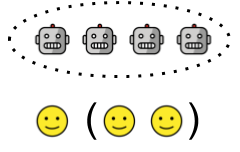
\includegraphics[width=\textwidth]{images/introduction/groups-robots.png}
        \caption{Groups of robots}
        \label{fig:groups-robots}
    \end{subfigure}
    \begin{subfigure}[b]{0.3\textwidth}
        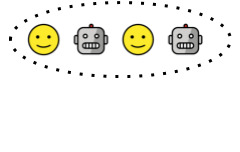
\includegraphics[width=\textwidth]{images/introduction/mixed-groups.png}
        \caption{Human-robot mixed groups}
        \label{fig:mixed-groups}
    \end{subfigure}
    \begin{subfigure}[b]{0.3\textwidth}
        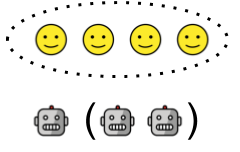
\includegraphics[width=\textwidth]{images/introduction/groups-humans.png}
        \caption{Robots near groups of humans}
        \label{fig:groups-humans}
    \end{subfigure}
    \caption{Structures of human-robot group interactions}
    \label{fig:group-interactions}
\end{figure}

\textcolor{blue}{Studying group interactions between humans and robots opens a wide range of challenges according to the nature and structure of those groups. We identified three distinct configurations of groups, see Figure~\ref{fig:group-interactions}, that lead to different types of interactions with robots. In Figure~\ref{fig:groups-robots}, \textit{groups of robots} represent the scenarios in which robots are expected to perform a task together around humans. The challenges in those situations may include exploring coordinated behaviour \cite{admoni2013dancing} or understanding how humans perceive robots in groups \cite{fraune2014negative}. In Figure~\ref{fig:mixed-groups}, \textit{human-robot mixed groups} depict scenarios in which robots act collaboratively alongside humans with similar goals. The challenges in those situations are usually focused on enhancing the collaboration and may range from signaling behaviour \cite{jung2013engaging} to support telepresence \cite{stoll2018wait}. Finally, in Figure~\ref{fig:groups-humans}, \textit{robots near groups of humans} illustrate scenarios in which the robot is required to act near a group of humans without being part of that group. The challenges may overlap with the mixed-groups, especially if the role of the robot is to provide assistance or facilitate the interaction. In those cases, the robot can also have a strong impact on the interaction among humans \cite{jung2018robot}. Examples of other challenges may include, for instance, the detection of group patterns \cite{leite2015comparing}.}



\textcolor{blue}{Overall, these research challenges contribute to successfully integrate robots in a society that is organised in groups. Robots will, therefore, be required to act in groups, to be part of groups alongside humans, or to be close to groups of humans. Jung and collaborators have proposed three broad research avenues to advance the study of group interaction in \gls{HRI} \cite{jung2017robots}. Firstly, understanding how the dynamics of existing group settings is shaped by a robot. In other words, analysing the impact robots have on the group processes, e.g. conflict or power. Secondly, understanding how the actual human-human interaction is influenced by robots. Finally, the last research avenue matches exactly the focus of this dissertation, which is how can robots mediate or enhance the performance of work groups or teams.}


\section{Group Dynamics}
As research on group interaction between humans and robots is still in its infancy, insights from other behavioural fields must be considered. In particular, the scientific study of all the processes that occur within and between interpersonal groups is called \textit{group dynamics}, which is being explored for the past century by several disciplines within the social sciences, e.g. organisational behaviour, social psychology, or management.

The social psychologist Forsyth defined a group as \textit{``two or more individuals who are connected by and within social relationships''} \cite{forsyth1990group}. He also pointed out the five main qualities of groups ---interaction, goals, interdependence, structure and cohesion--- and the fact that each one of them provides complex and fascinating phenomena when analysed more closely. According to these key qualities, a group interacts or sustains a relationship in order to achieve a certain purpose or outcome. It is usually structured in a way that its members have interdependent roles or relations that remain together due to a cohesive alliance. There is, however, a particular type of groups that intensifies these five qualities to an extreme level ---teams. Members of a team are usually committed to a common goal in which the individual success is only a consequence of the collective success. There is a strong interdependence of their efforts that requires a coordinated interaction. In terms of structure, teams usually present highly adaptive skills that allow a revision of their norms and procedures in order to improve their functioning. Finally, the cohesive alliance of a team is also a salient characteristic, as Forsyth defines teams as \textit{``unified, cohesive groups''}.



\section{Research Problem}
As previously mentioned, teams are a particularly strong type of groups, in the sense that members of a team experience intense relations towards their shared goal. Nevertheless, as teamwork and collaboration do only require a team to have at least two entities, most \gls{HRI} literature in this topic is focused on dyadic collaborations \cite{hoffman2007effects,dragan2015effects,huang2016anticipatory,chang2018effects,shayganfar2019appraisal,hoffman2019evaluating}. The exploration of teamwork and collaboration within small groups of humans and robots (i.e. groups with more than one person and/or more than one robot) is still scarce \cite{fraune2017teammates}.

Although robots can easily outperform humans when individually executing specific tasks, e.g. \cite{butner2003transforming} or \cite{cicconet2012visual}, achieving satisfactory and effective collaborations might not be straightforward \cite{bauer2008human}. As soon as robots start working close to humans or are required to collaborate with them, their social capabilities become not only useful but also necessary. Dautenhahn et al. extensively revisited the definition of socially embedded agents which are tightly coupled to the social environment \cite{dautenhahn2002embodied}. The authors further proposed these agents can ``benefit from possessing some degree of awareness of the social system, i.e. a means of perceiving and sensing structures within the social world, and means of acting within it''. This thesis aims at contributing to this notion of socially embeddedness, specifically in relation to the group dynamics of an environment where the robot is required to be a team member.



%argument why now measuring performance
An immediate question that might occur is: what exactly is \textit{the effectiveness} of a mixed human-robot team? An intelligible answer can be that it is highly dependent on task itself, the purpose or the goals of the team. Therefore, we acknowledge that there might be several different ways of assessing effectiveness. One possibility is maximising the performance achieved by the team, which is mostly the main motivation for developing robotic teammates. There are, however, other possibilities such as examining other aspects or factors that sustain the quality of the team and may, in turn, mediate performance. One of those factors is certainly cohesion, pointed by many authors as the most important aspect of groups and, consequently, of teams. It is considered the integrity, solidarity and unity that maintains a group together or, in other words, the ``groupiness of a group''. Cohesion is associated with satisfaction, performance, and productivity. For instance, Mullen and Cooper found an interesting bidirectional relationship between cohesion and performance, which suggests that not only cohesive teams tend to perform better, but also the success of the team leads to increased cohesion \cite{mullen1994relation}.


Additionally, there are many complex tasks in which the performance or the outcome achieved by the team is affected, or even damaged, by external factors. And yet, the integrity of a team may be strong enough to sustain satisfaction and the \textit{esprit de corps} in those situations. As a result, we are interested in this particular type of cohesive alliance in mixed teams of humans and robots and we have formulated our research problem as follows.

\begin{indented}
%In a mixed human-robot team setting, how can a social robot establish and improve a cohesive alliance with the other team members?%How can we create an effective robotic teammate? In particular, how are cohesive alliances established with robotic teammates and
How can we endow a social robot with the ability to improve the cohesive alliance in a team setting with humans?
\end{indented}

An initial consideration to undertake this research problem is the understanding of how humans establish cohesive alliances in their interpersonal groups or teams. The multi-dimensionality of the \textit{cohesion} construct suggests that there are five possible courses that lead to cohesiveness: the task, the social bonds, the collective entity, the structure and emotions. \textit{Task cohesion} emerges from the shared commitment towards a common goal, while \textit{social cohesion} develops from the attractions among the members. The identification of the members with the group and the degree of belonging constitutes the \textit{collective cohesion}. The \textit{structural cohesion} derives from the norms, roles and relationships that link the members of the group. Finally, \textit{emotional cohesion} is the intensity of the members to express group feelings. In this thesis, we will explore the first four types or dimensions of cohesion.

Overall, this research problem can be tackled in many different ways, especially considering the multi-dimensionality of the cohesion construct. Therefore, it is important to clarify what are the research directions that this dissertation will undertake. The challenges or goals that we address are twofold. On the one hand, (a) \textit{to evaluate the impact of the robot's social behaviours on the cohesion of the team}. This first research goal aims at understanding the evolution and development of teams with humans and robots. It includes the analysis of how do people perceive the robotic teammate, how does the behaviour of the robot influence the team, or even how do external factors affect those perceptions. On the other hand, (b) \textit{to develop computational mechanisms to autonomously increase the cohesive alliance of a mixed team of humans and robots}. This second research goal is focused on the computational aspects that facilitate the robotic agent to autonomously improve the cohesion of its team. These mechanisms may affect both its decision-making and its perceptive skills to analyse and model the group.



\section{Contributions}
This dissertation holds four major contributions that address the two aforementioned goals:

\begin{itemize}
    \item[1.] \textbf{Evaluate the impact of the robot's social behaviours on the social cohesion of the team} - Social cohesion develops from the attractions of group members both at individual- and group-level. Those attractions can flourish when team members have particular traits, for instance. However, what exactly are the traits that we seek in robotic teammates? Based on the learning-goal theory, we created two distinct characters for social robots to either express a performance goal or a learning goal, which translate into more competitive or more relationship-driven behaviours. We conducted a user study using a card-game where human players could form a team with each robotic character. By exploring different team formations, we contribute to the understanding of membership preferences towards robotic teammates, which is detailed in Chapter~\ref{chapter:membership-formation}.
    
    
    \item[2.] \textbf{Evaluate the impact of the team's outcome on the collective cohesion} - Collective cohesion reflects the degree of identification with the group. It is usually mentioned as the replacement of the ``I'' by the ``we'' and, when this feeling becomes stronger, it may even affect one's actions with the collective goals taking priority over the individual ones. We aim at exploring how people perceive different levels of collective cohesion on robotic teammates and how those are influenced by the achieved outcome being positive or negative. Chapter~\ref{chapter:pro-sociality} presents a user study that explores this research question in a Public Goods Game between a mixed team of one human and two robots. The results contribute with important considerations to the understanding of collective cohesion in teams of humans and robots.
    
    \item[3.] \textbf{Develop computational mechanisms for the robotic teammate to improve collective cohesion} - According to the group identity theory, there is a group of emotions that reflects a high level of identification with the group, which are called the \textit{group-based emotions}. Chapter~\ref{chapter:group-based-emotions} describes a computational approach to implement the group identity theory on an emotional agent in order to express this type of emotions. It also contributes with a user study that evaluates the proposed model on a robotic teammate and its impact on the collective cohesion of the team.
    
    \item[4.] \textbf{Develop computational mechanisms for the robotic teammate to autonomously perceive the structural cohesion of the team} - The structure of a team can be represented in a graph where nodes correspond to the team members and the links may identify different types of relations, such as roles, norms, or interactions. Usually, the density and topology of those structures is associated with the degree of cohesion of a team. We plan to extend the perceptive skills of a social robot to detect the communication network of the team members. Such mechanism will allow the robotic teammate to autonomously perceive aspects of the group related with its structural cohesion. Chapter~\ref{chapter:future-work} proposes an approach to address this last contribution of this dissertation.
\end{itemize}



\section{Roadmap}
The current document contains 7 chapters and is organised as follows. %\textbf{Chapter~\ref{chapter:background}} provides relevant and central notions on interpersonal cohesion, which will support the further reading of the current document. 
In \textbf{Chapter~\ref{chapter:related-work}}, we present the state-of-the-art on group interactions between humans and robots. The following three chapters, \textbf{Chapter~\ref{chapter:membership-formation}}, \textbf{Chapter~\ref{chapter:pro-sociality}}, and \textbf{Chapter~\ref{chapter:group-based-emotions}}, detail our previous work, corresponding to contributions 1, 2 and 3, respectively. The fourth and last contribution corresponds to the future work of this ongoing dissertation and the proposed approach to address it is presented in \textbf{Chapter~\ref{chapter:future-work}}.

Finally, the document ends in \textbf{Chapter~\ref{chapter:conclusion}} with a discussion and concluding remarks on the current contributions of this thesis and a proposal to address our last research goal 2.2, that constitutes our on-going work.

%%!TEX root = ../dissertation.tex

\chapter{Background}
\label{chapter:background}

Groups...

Teams...

Cohesion...


\chapter{Related Work}
\label{chapter:related-work}

In this chapter, we review the state-of-the-art of group interactions between humans and robots. We identified four main topics among the reviewed literature, which constitute the first four sections of the current chapter. The last section contributes with a comparative analysis and an overview of the expected contributions of this dissertation.



\section{Group Identity, Membership and Social Categorisation}
\label{sec:identity}
Group identity is one of the most fundamental aspects of a group as it defines its formation and membership. In other words, it is responsible for the categorisation of individuals as part of a larger identity or group. Group identification is also associated with many group processes and, therefore, researchers interested in human-robot group interaction have been playing close attention to it.

Eyssel \& Kuchenbrandt pioneered the exploration of social categorisation in HRI. They manipulated social categorisation with the background information of the robot, i.e., nationality and name \cite{eyssel2012social}. Participants reported their perceptions of the robot after seeing a picture of it. The salience of that group membership was enough for participants to rate the ingroup robot more favourably and anthropomorphise it more.

In a similar experiment, Kuchenbrandt et al. manipulated group identity by simply associating colours to two groups, the minimal-group paradigm, and the robot would either be from the ingroup or the outgroup \cite{kuchenbrandt2013robot}. Participants were greeted with a short introduction by the robot and then rated their perceptions of it. Participants that interacted with the ingroup robot attributed significantly more anthropomorphism to it and even revealed higher willingness to interact with robots in general, compared to the ones that interacted with the outgroup robot.

One of the experiments presented by Deligianis et al. also explored the minimal group paradigm by simply priming participants about a presumed ``robot condition'' or a ``computer condition'' \cite{deligianis2017impact}. Participants had to play the shell game in a team with a robot that occasionally disagreed with the participant's answer to measure trust or compliance with that suggestion. Moreover, the difficulty of the game was manipulated in two levels, medium and hard. The results confirmed their first hypothesis stating that participants would trust the robot more often when the game difficulty was harder. Regarding the manipulation of the ingroup, it influenced the proxemics between the participants and the robot after the game, but no significant differences were found in trust to comply with the robot's suggestions.

The minimal group paradigm has not been always successful to induce the group membership. Sembroski et al. run a user study with a medical diagnosis task in which the robot would either be presented as a teammate (ingroup) or as a provider of additional information (outgroup) \cite{sembroski2017he}. The goal of this user study was to analyse participants' willingness to follow the robot's instructions. Nevertheless, the manipulation check of group membership did not reveal significant differences between these two experimental groups suggesting the nature of the task might have conditioned this perception.


Recently, Steain et al. presented the results of a user study where they have analysed social categorisation in the shell game \cite{steain2019black}. The manipulation of identity was achieved by introducing the robots as ``EngBot'' and ``PsycBot'' to a population of students from psychology. The results of the experiment were focused on the perceptions of the robots and the degree of compliance with the answers of each robot i.e., trust. Although no significant differences were found for trust, participants rated the ingroup robot more favourably, kept a closer distance and preferred it more compared to the outgroup robot.


The identification towards a certain group can emerge from social aspects, as well as task-related aspects. As a result, several group identities can be present at the same time. In light of this idea, Haring et al. explored both task structure i.e., robotic partner or competitor, and the social membership, manipulated by the nationality of the robots \cite{haring2014would}. In their user study, participants had to play a card game with two robots, where one of them was their teammate and the other was their opponent. Participants were told each robot was developed by a team of either their own nationality (ingroup) or another one (outgroup) and the names of the robots would also match their alleged nationality. The two experimental conditions mapped the congruency between social membership of the robots and their role in the game: ingroup partner and outgroup opponent; and outgroup partner and ingroup opponent. Results identified a main effect of the social membership on the perception of competence and on the cooperation index, with participants rating the ingroup robot as more competent and cooperated more with it compared to the outgroup robot. A surprising result of this user study was the fact that participants reported higher closeness to the ingroup robot when it was their partner compared to when it was their opponent but no similar difference occurred for the outgroup robot.


Finally, Fraune et al. presented the results of a user study whose goal was to compare the membership towards humans and robots. In their experiment, two teams of two people and two robots each had to competitively play a price-guessing game \cite{fraune2017teammates}. The main goal of this user study was to compare the perception and behaviour towards the ingroup and outgroup members, which was inherently set by the competitive setting. Additionally, it explored differences between robotic and human members. The results in terms of anthropomorphism and perceptions of cooperation support a strong impact of the ingroup setting compared to the outgroup, regardless of being a robot or a human. However, there was a surprising interaction effect on the aggression measure which was a noise blast that participants could use to damage partners or opponents during the game. Participants favoured the ingroup human over the ingroup robots, but they also favoured ingroup robots over outgroup humans. To a certain extent, this result indicates that people can favour robots over humans in some competitive settings.



\section{Group Phenomena in HRI}
\label{sec:phenomena}
Another line of research that we identified in the literature of human-robot group interactions is a set of user studies trying to verify if well-known group phenomena from the social sciences also applies to HRI. Therefore, the commonality among the following user studies is a comparison between individuals and groups of humans interacting with robot(s).

Chang et al. examined if the discontinuity effect translates into human-robot interactions \cite{chang2012effect}. This effect suggests that interactions among groups of humans are more competitive than interactions among individuals. The user study manipulated the number of people in one team (either 1 or 2) and the number of robots in the adversarial team (also either 1 or 2). The interaction consisted of a board game with occasional social dilemmas between the teams to measure competitiveness. The results do not fully support the discontinuity effect in HRI but only than increasing the number of people increases competitiveness.

In a similar experiment, Fraune et al. have also analysed the discontinuity effect \cite{fraune2019human}. Participants, individually or in a group of three, engaged in a social dilemma against a either a single robot or a group of three robots. The goal of this user study was to analyse the perceptions of the participants, as well as their competitiveness, in each of four experimental conditions. Contrary to human-human interaction, where increasing the number of members in at least one group would increase competitiveness, the results of this user study suggest a different pattern in human-robot interaction. In the two conditions where both teams had the same size, individual vs. individual and group vs. group, the competitiveness was higher. Additional results revealed that participants that played in groups of three had more negative emotions and competed more with the robot(s), compared to participants playing individually. Moreover, they found a positive correlation between the entitativity of the human group and the competitiveness, and also between the entitativity of the robot group and the reported fear.

Another interesting group phenomenon is comformity, which occurs in group interactions when a member changes his opinion or action in order to increase the consistency with other group members. This phenomenon illustrates how group processes may go beyond individual processes and how complex group interactions can be. Brandstetter et al. investigated if robots were also able to produce conformity behaviours in humans \cite{brandstetter2014peer}. In their experiment, a group of 5 people was compared to a group of one person and four robots. The task was a linguistic quiz to identify past tenses. Although participants exhibited conformity with human peers, they did not display with the robots.

Solomons et al. have also explored conformity effect within a group of a human and three robots playing the Dixit game \cite{salomons2018humans}. In their modified version of the game, a fourth robot was always the game master and would say a new word every round for the players to guess the corresponding card. There were two conditions: one where the participant could see which card was voted by the other robots and change his original decision; and a control condition in which the participant could not see the decisions of the robotic players. The results suggested that people have indeed conformed with the robots' responses in the experimental group. Additionally, the authors discussed a possible explanation for the incongruent result with Brandstetter et al. related to trust. They postulated trust plays an important role to perform conformity behaviours as robot started to choose incorrect answers and participants stopped conforming later in the game.

Interpersonal groups can outperform individuals in a variety of tasks and can, sometimes, even display higher learning gains. In order to explore this idea, Leite et al. have examined a learning activity between children and robots in an interactive storytelling scenario \cite{leite2015emotional}. In particular, they have compared a single child with a group of three children in terms of story recall and the emotional interpretation of the story content. The results revealed that participants interacting alone presented higher levels of recall, compared to participants in the group condition. The authors speculated some possible reasons, for instance, group interaction may require children to work on their social standing, which may have compromised their attention.

Finally, a recent in-the-wild experiment revealed several human factors affecting human-robot interactions, including the number of people within the group \cite{fraune2019humangroup}. In this user study, Robovie was deployed in a Japonese shopping mall with the purpose of giving directions to people. Video recordings of 2714 participants and surveys responses of 78 participants were collected and extensively analysed. The results showed that people interacting with the robot in groups, especially the entitative groups, (1) interacted more and for longer periods, (2) behaved more socially towards the robot, and (3) were more positive, compared to people interacting alone. Additionally, people in groups displayed compliance with social norms of the group, for instance, when someone in the group interacted with the robot, the others were likely to interact as well.



\section{Perceptions of Groups of Robots}
\label{sec:perceptions}
Robots may be required to perform or execute tasks in groups without human intervention or collaboration. Nevertheless, they will certainly be deployed in social settings and be surrounded by humans, whose perceptions and expectations might constrain their behaviour. As a result, this section overviews research on how people react to and perceive groups of robots. 

Admoni et al. analysed different conformity levels in groups of robots and how they impact the perceptions of humans \cite{admoni2013dancing}. Participants saw videos of robots performing a dance routine where one of them was dancing independently while the others were coordinated and synchronised. They manipulated the size of the group to have either four or eight robots in order to increase the sense of majority and minority (3+1 and 7+1). Additionally, there was a control condition with only two robots with opposing dances. The dance type was also manipulated so that the minority robot could be dancing unique and distinct dance moves, similar moves but in a difference order, following the exact same moves but behind time, or leading the exact same moves ahead of time. Results showed the minority robot was consistently rated as less of a team-player and more anti-social, but more creative as well. This team-player measure was exacerbated when the group size increased. However, the differences across the four dance types were not statistically significant.

Behavioural mimicry was also analysed with other two factors, appearance and eye gaze, by Nawroj and collaborators \cite{nawroj2014exploration}. Participants of the user study saw videos of three robots performing a dancing routine (robots A, B and C) and were only asked to rate the groupiness of robot C. The mimicry variable was manipulated for the robot C to either mimic A, B or none. Similarly, appearance and gaze were also manipulated for the robot C to either look like and gaze at A, B or none. As a result, there were 27 different videos of the robots dancing and each participant saw and rate nine of them. The results highlighted a strong main effect of behavioural mimicry, even when it interacted with conflicting cues from the appearance and gaze. Additionally, there was also a main effect of the appearance variable while mutual-gaze was not a significant predictor of grouping patterns.

Fraune \& {\v{S}}abanovi{\'c} explored the perceptions of people towards a group of three robotic vacuum cleaners \cite{fraune2014negative}. The user study manipulated in a between-subjects design the communication style among the robots, which could either be silent, loud, or no communication at all. The results revealed no significant differences between the attitudes towards robots, as well as on the perceived social attributes o the robots. Moreover, in the manipulation check questions, participants could not identify differences in the communication style of the robots. The authors speculate that the non-humanoid embodiment of the Roomba as well as the low sociability of the robots might have strongly influenced the lack of differences.

Later, the same authors and collaborators investigated the role of embodiment when comparing a single robot with a group of robots \cite{fraune2015rabble}. They run a user study in which videos of the robots were shown to people and their perceptions were assessed in subjective questionnaires. In a between-subjects design, the video displayed either a single robot or a group, which could in turn have a humanoid embodiment (NAO), zoomorphic (Pleo) or mechanomorphic (Roomba). The results revealed an interaction effect between the two variables, group size and embodiment type. Groups of Roomba robots increased the negative responses, such as threat, anxiety or fear, compared to a single Roomba robot. On the other hand, The groups of NAO robots were positively rated in terms of elicited affect, perceived threat and trust, compared to a single NAO robot. Finally, the comparison between a single Pleo and the group of Pleo robots did not reveal differences in affective states but rather in the description traits (i.e., stereotypes) and future work contexts.

In their demand to understand the factors influencing the perceptions of robots in groups, Fraune and collaborators conducted another experiment where sociable trash robot entered the a public space, the cafeteria of the university \cite{fraune2015three}. They assessed behavioural and subjective measures of participants interacting with the robots and manipulated the number of robots, either one or a group of three, and different robotic behaviours, social or functional. The social behaviours consisted of contingent behaviour towards participants, such as greeting with a bow or a nod and a nonverbal ``thank you'' for throwing trash. A main effect of the number of robots revealed that a group of robots induced more direct interaction and more trash being thrown. Similarly, the main effect of the behaviour also shown that functional behavioural elicited longer gazes by people and more trash being thrown. Overall people preferred single social robots and groups of functional robots.

Finally, the last contribution of Fraune and collaborators to this line of research includes an experiment on the impact of group entativity \cite{fraune2017threatening}. Participants engaged in an object-matching task and the robot, or group of robots (depending on the condition), would assert their ability to perform the task. There were three conditions: a single robot, an entitative group and a diverse group. Entitativity was manipulated by the appearance, motion, proximity and decisions of the robots. The entitative group was perceived as more threatening than both the diverse group and the single robots. Moreover, the entitative group was also perceived more negatively when compared to the single robots only. On the other hand, participants attributed more mind to the diverse group than single robots.



\section{Robotic Group Behaviour}
\label{sec:behaviour}
Providing autonomy to social robots in group interactions can be a challenging task as it may include perceptive, cognitive and decision-making capabilities. The findings of the following reviewed papers contribute to the scope of literature that understands how robots can perceive and act in group settings with humans.

Leite et al. have contributed to enhancement of robotic perceptions in group interactions \cite{leite2015comparing}. The authors collected data of children playing an interactive storytelling activity with two robots in two distinct conditions: one where children participated alone and another where children participated in groups of three. Then, they developed two predictive models of individual disengagement, one trained with data from single interaction condition and another from group interaction condition. The annotations of engagement were done by human coders. Their analysis is focused on the evaluation of the two predictive models in both datasets in order to investigate how well the model trained on single interaction performs in group interaction and vice-versa. The disengagement model trained from group interactions performed reasonably well in the single interaction dataset, while the opposite could not be validated.

Jung et al. explored backchanneling behaviour in human-robot teamwork \cite{jung2013engaging}. They run a user study where a team of 5 members (3 robots, 1 participant and 1 human confederate) had to retrieve items from a building that has allegedly collapsed. In a between-subjects design, they manipulated both the presence of backchanneling behaviour and the task complexity. Results showed that when robots employed the backchanneling behaviour, they were perceived as more engaged to the task and their human partners reported lower stress levels as well as lower cognitive load, especially for the complex task. However, the backchanneling behaviour decreased the perception of competence of the robots. Overall, it seems that backchanneling can positively influence human-robot teamwork at a certain cost, and it is mostly beneficial in complex or demanding task.

Another sort of nonverbal behaviour was also explored by Vázquez et al. that examined how a robot is perceived during a group conversation according to its body orientation and gaze direction \cite{vazquez2017towards}. They run a user study in which groups of three participants had to brainstorm about possible tasks or purposes for the robot. Participants were briefed and debriefed by the robot and during the group discussion, it pretended to be listening and paying attention to conversation. Both the orientation and gaze of robot were manipulated in a between-subjects design. Orientation could be towards the middle of the conversation group or towards the participant that had the conversational floor, while gaze could be random or also attentive towards the participant that had the conversational floor. Although participants in the four experimental groups reported similar feelings of inclusion and belonging to the group, the gaze affected participants' perception of the robot motion, as well as the orientation affected the perception of its gaze. These results suggest gaze and orientation should be jointly design and controlled.

Conflict is believed to be an important stage of group development \cite{forsyth1990group} and the resolution of conflict is associated with several measures of group performance \cite{jung2016coupling}. Recently, Jung et al. have looked at how the emotional behaviour of a robot can have a positive impact on improving teamwork by employing emotion regulation strategies to diffuse conflict situations \cite{Jung2015}. The results suggested that although the robot's repair interventions have increased the groups' awareness of conflict, they can aid the conflict regulating process of the team.

Similarly, Shen et al. analysed the impact of a robotic mediator during conflict resolution among children \cite{shen2018stop}. In their experiment, pairs of children played five activities during 50 minutes that were facilitated by the robot. In a between-subjects design, they manipulated whether the robot would or not display an additional conflict mediation when children engaged in object possession conflicts. The procedure for the robot to intervene consisted of three steps: (1) play a whilst sound and identify the conflict; (2) offer prompts for constructive conflict resolution; and (3) wrap up and move forwards from the conflict. Results have shown that children were more likely to solve the conflicts constructively in the condition where the robot mediated the conflicts compared to the control condition.

Social robots can have different roles in the the way they interact with humans, from partners to opponents, or even have mixed-motive goals to mere facilitators or mediators. Tennent et al. have recently investigated whether a peripheral robotic microphone can positively shape the interpersonal dynamics of a team during a problem solving task \cite{tennent2019micbot}. They run a user study in which the robot displayed one of three possible behaviours: no movement, random, and engagement. The engagement behaviour balanced between following who had the conversational floor and encouraging the participant who had spoke the least. Results showed that in the engagement condition, the conversational dynamics was more even compared to the no movement. Curiously, there were no significant differences between the random condition and the engagement, nor between the random and no movement. This suggest the behaviour of the robot might have to be somehow socially contingent in order to differ from the stationary robot. Additionally, they found a correlation between the unevenness measure and team performance. Overall, the engagement behaviour produced more balanced discussions among the team and led to better team performance.

Finally, another work explored a mediation role by a social robot that was assisting a team of two humans in a tower construction task. In particular, Jung et al. examined different resource allocation algorithms and their impact on the task execution \cite{jung2018robot}. In their user study, the robot could either equally distribute the blocks among the two team members or execute an unequal distribution by giving 65\% of the blocks to one participant and 35\% to the other. The results revealed that team members in equal distribution reported a significantly more positive interpersonal relationship than team members in the unequal distribution condition.



\subsection{Analysis of Human-Robot Group Interaction}
The scope of papers we have reviewed highlights a diversity of topics within human-robot group interaction. Beyond the categorisation we have created in the previous sections, there are other interesting ways to analyse group interactions regarding the type of tasks involved, the structure of the group itself, and the role of the robot(s).

In order to perform such comparison, we have used the circumplex of group tasks proposed by McGrath \cite{mcgrath1995methodology}, see Figure~\ref{fig:circumplex}. This model for classifying group tasks has eight octants along the two dimensions of \textit{generate-negotiate} and \textit{choose-execute}. In the generate quadrant, tasks can either be \textit{creative} if the goal is to generate ideas, or of \textit{planning} type if the goal is to elaborate a plan. In the choose quadrant, the task is to solve a problem that can either have, or not have, correct answers, \textit{intellective} or \textit{decision making}, respectively. In the negotiate quadrant, the tasks require conflict resolution and the octants depend on the nature of the conflict. It is a \textit{cognitive conflict} in case of conflicting viewpoints and it is considered a \textit{mixed motive} in case of conflicting interests. Finally, in the execute quadrant, tasks can either be \textit{competitions} or of \textit{performance} type if it involves resolving conflicts of power or execute a performance or psychomotor task, respectively.

\begin{figure}
    \centering
    \begin{tikzpicture}
        \draw[<->] (-5,0) node[rotate=90, above]{$II. Choose$} --(5,0) node[right]{$IV. Execute$} ;
        \draw[<->,] (0,-5)node[below]{$III. Negotiate$} --(0,5) node[above]{$I. Generate$};
        \draw (0,0) circle (4);
        \draw[-] (-3,3)--(3,-3);
        \draw[-] (-3,-3)--(3,3);
        \node[rotate=337.5] at (2,4)  {Planning};
        \node[rotate=292.5] at (4,2)  {Performance};
        \node[rotate=247.5] at (4,-2)  {Competitions};
        \node[rotate=202.5] at (2,-4)  {Mixed Motive};
        \node[rotate=157.5] at (-2,-4)  {Cognitive Conflict};
        \node[rotate=112.5] at (-4,-2)  {Decision Making};
        \node[rotate=67.5] at (-4,2)  {Intellective};
        \node[rotate=22.5] at (-2,4)  {Creative};
        \node[draw,circle,inner sep=1pt,color=cyan] at (-3.5,0.5) {\cite{fraune2017teammates}}; %2
        \node[draw,circle,inner sep=1pt,color=cyan] at (-2.7,0.5) {\cite{deligianis2017impact}}; %4
        \node[draw,circle,inner sep=1pt,color=cyan] at (-3.5,-0.5) {\cite{sembroski2017he}}; %5
        \node[draw,circle,inner sep=1pt,color=violet] at (0.5,-3.5) {\cite{fraune2019human}}; %6
        \node[draw,circle,inner sep=1pt,color=cyan] at (-2.7,-0.5) {\cite{haring2014would}}; %7
        \node[draw,circle,inner sep=1pt,color=violet] at (0.5,-2.7) {\cite{chang2012effect}}; %8
        \node[draw,circle,inner sep=1pt,color=violet] at (-1.9,0.5) {\cite{brandstetter2014peer}}; %13
        \node[draw,circle,inner sep=1pt,color=violet] at (-1.9,-0.5) {\cite{salomons2018humans}}; %15
        \node[draw,circle,inner sep=1pt,color=cyan] at (-3.1,1.2) {\cite{steain2019black}}; %16
        \node[draw,circle,inner sep=1pt,color=darkgreen] at (0.5,-1.9) {\cite{shen2018stop}}; %17
        \node[draw,circle,inner sep=1pt,color=orange] at (3.5,0.5) {\cite{fraune2014negative}}; %18
        \node[draw,circle,inner sep=1pt,color=orange] at (2.7,0.5) {\cite{admoni2013dancing}}; %19
        \node[draw,circle,inner sep=1pt,color=orange] at (1.9,0.5) {\cite{fraune2015rabble}}; %20
        \node[draw,circle,inner sep=1pt,color=orange] at (-2.3,1.2) {\cite{fraune2017threatening}}; %21
        \node[draw,circle,inner sep=1pt,color=orange] at (1.1,0.5) {\cite{Fraune-RSS-15}}; %22
        \node[draw,circle,inner sep=1pt,color=violet] at (-1.1,0.5) {\cite{leite2015emotional}}; %23
        \node[draw,circle,inner sep=1pt,color=violet] at (0.5,3.5) {\cite{fraune2019humangroup}}; %24
        \node[draw,circle,inner sep=1pt,color=darkgreen] at (3.1,1.2) {\cite{jung2013engaging}}; %25
        \node[draw,circle,inner sep=1pt,color=orange] at (2.3,1.2) {\cite{nawroj2014exploration}}; %26
        
        \node[draw,circle,inner sep=1pt,color=darkgreen] at (-2.7,1.9) {\cite{leite2015comparing}}; %27
        \node[draw,circle,inner sep=1pt,color=darkgreen] at (-1.5,1.2) {\cite{tennent2019micbot}}; %29
        \node[draw,circle,inner sep=1pt,color=darkgreen] at (2.7,1.9) {\cite{jung2018robot}}; %30
        \node[draw,circle,inner sep=1pt,color=darkgreen] at (-0.5,3.5) {\cite{vazquez2017towards}}; %31
        \matrix [draw,below left,font=\small] at (current bounding box.north east) {
          \node [shape=circle, draw=cyan,label=right:Group Identity] {}; \\
          \node [shape=circle, draw=violet,label=right:Group Phenomena] {}; \\
          \node [shape=circle, draw=orange,label=right:Groups of Robots] {}; \\
          \node [shape=circle, draw=darkgreen,label=right:Group Behaviour] {}; \\
        };
    \end{tikzpicture}
    \caption{Reviewed papers in the Circumplex of Group Tasks \cite{mcgrath1995methodology}}
    \label{fig:circumplex}
\end{figure}

Most of the works exploring group identity and group membership (blue references in Figure~\ref{fig:circumplex}) are located in the \textit{choose} quadrant, revealing the nature of those tasks requires people to perform some kind of decision. The manipulations of group identity or the simple social categorisations were achieved by either the minimal group paradigm or by the structure of the group, i.e., people forming teams with the robots. Additionally, we also noticed that the most common role for the robot(s) in this set of papers is the being a peer or a teammate. Consequently, the predominant structure or composition of these groups is human-robot mixed groups.

The second group of papers we have analysed (violet references in Figure~\ref{fig:circumplex}) corresponds to the exploration of group phenomena in HRI. There is no predominant type of task among the reviewed papers. Nevertheless, there seems to be a tendency to explore the role of a competitor. Most of the discussed scenarios attributed similar goals to both humans and robots in a way that they compete for resources either implicit- or explicitly.

Regarding the perceptions of groups of robots (orange references in Figure~\ref{fig:circumplex}), we noticed that most tasks are located in the \textit{performance} octant. The papers reviewed in this category discuss the perceptions people had seeing groups of robots executing a certain task, or videos of those performances, without requiring any human intervention. Therefore, it is hard to assess a specific role for robots in those situations. Nonetheless, as mere performers, such as the vacuum cleaner or the robotic trash bin, they can be seen as servants or subordinates.

Finally, the papers within the category of group behaviour cover several types of tasks (green references in Figure~\ref{fig:circumplex}), including the uncommon creative type. Interestingly, we noticed a trend in the role of the robot(s) in this set of papers, which is a mediator or a facilitator.
When the robot mediates or facilitates the interaction, its goal is somehow complementary to the humans and, therefore, it is strong enough to influence and shape the interaction.


\subsubsection{Expected contributions}

Figure~\ref{fig:circumplex-contributions} revisits the circumplex of group tasks and adds the expected contributions of this dissertation. The \textit{contribution A}, which is detailed in Chapter~\ref{chapter:membership-formation}, explores group formation, membership preferences, and perceptions of robotic teammates in a decision making task. Secondly, \textit{contribution B}, detailed in Chapter~\ref{chapter:pro-sociality}, explores the perceptions of robotic teammates that favour different interests in a mixed motive task. \textit{Contribution C}, presented in Chapter~\ref{chapter:group-based-emotions}, adds to the literature of group behaviour by exploring the generation of group-based emotions in robotic teammates during a decision making task. Finally, \textit{contribution D}, which is the future work of this ongoing dissertation and detailed in Chapter~\ref{chapter:future-work}, aims at contributing as well to group behaviour, but in a mixed motive task.

\begin{figure}
    \centering
    \begin{tikzpicture}
        \node[draw,circle,inner sep=1pt,color=cyan] at (-3.5,0.5) {\cite{fraune2017teammates}}; %2
        \node[draw,circle,inner sep=1pt,color=cyan] at (-2.7,0.5) {\cite{deligianis2017impact}}; %4
        \node[draw,circle,inner sep=1pt,color=cyan] at (-3.5,-0.5) {\cite{sembroski2017he}}; %5
        \node[draw,circle,inner sep=1pt,color=violet] at (0.5,-3.5) {\cite{fraune2019human}}; %6
        \node[draw,circle,inner sep=1pt,color=cyan] at (-2.7,-0.5) {\cite{haring2014would}}; %7
        \node[draw,circle,inner sep=1pt,color=violet] at (0.5,-2.7) {\cite{chang2012effect}}; %8
        \node[draw,circle,inner sep=1pt,color=violet] at (-1.9,0.5) {\cite{brandstetter2014peer}}; %13
        \node[draw,circle,inner sep=1pt,color=violet] at (-1.9,-0.5) {\cite{salomons2018humans}}; %15
        \node[draw,circle,inner sep=1pt,color=cyan] at (-3.1,1.2) {\cite{steain2019black}}; %16
        \node[draw,circle,inner sep=1pt,color=darkgreen] at (0.5,-1.9) {\cite{shen2018stop}}; %17
        \node[draw,circle,inner sep=1pt,color=orange] at (3.5,0.5) {\cite{fraune2014negative}}; %18
        \node[draw,circle,inner sep=1pt,color=orange] at (2.7,0.5) {\cite{admoni2013dancing}}; %19
        \node[draw,circle,inner sep=1pt,color=orange] at (1.9,0.5) {\cite{fraune2015rabble}}; %20
        \node[draw,circle,inner sep=1pt,color=orange] at (-2.3,1.2) {\cite{fraune2017threatening}}; %21
        \node[draw,circle,inner sep=1pt,color=orange] at (1.1,0.5) {\cite{Fraune-RSS-15}}; %22
        \node[draw,circle,inner sep=1pt,color=violet] at (-1.1,0.5) {\cite{leite2015emotional}}; %23
        \node[draw,circle,inner sep=1pt,color=violet] at (0.5,3.5) {\cite{fraune2019humangroup}}; %24
        \node[draw,circle,inner sep=1pt,color=darkgreen] at (3.1,1.2) {\cite{jung2013engaging}}; %25
        \node[draw,circle,inner sep=1pt,color=orange] at (2.3,1.2) {\cite{nawroj2014exploration}}; %26
        
        \node[draw,circle,inner sep=1pt,color=darkgreen] at (-2.7,1.9) {\cite{leite2015comparing}}; %27
        \node[draw,circle,inner sep=1pt,color=darkgreen] at (-1.5,1.2) {\cite{tennent2019micbot}}; %29
        \node[draw,circle,inner sep=1pt,color=darkgreen] at (2.7,1.9) {\cite{jung2018robot}}; %30
        \node[draw,circle,inner sep=1pt,color=darkgreen] at (-0.5,3.5) {\cite{vazquez2017towards}}; %31
        \fill[white, opacity=0.7] (-4,-4) rectangle (4,4);
        \draw[<->] (-5,0) node[rotate=90, above]{$II. Choose$} --(5,0) node[right]{$IV. Execute$} ;
        \draw[<->,] (0,-5)node[below]{$III. Negotiate$} --(0,5) node[above]{$I. Generate$};
        \draw (0,0) circle (4);
        \draw[-] (-3,3)--(3,-3);
        \draw[-] (-3,-3)--(3,3);
        \node[rotate=337.5] at (2,4)  {Planning};
        \node[rotate=292.5] at (4,2)  {Performance};
        \node[rotate=247.5] at (4,-2)  {Competitions};
        \node[rotate=202.5] at (2,-4)  {Mixed Motive};
        \node[rotate=157.5] at (-2,-4)  {Cognitive Conflict};
        \node[rotate=112.5] at (-4,-2)  {Decision Making};
        \node[rotate=67.5] at (-4,2)  {Intellective};
        \node[rotate=22.5] at (-2,4)  {Creative};
        \node[draw,circle,inner sep=1pt,color=cyan,ultra thick,font=\bfseries] at (-3,-1.6) {A};
        \node[draw,circle,inner sep=1pt,color=cyan,ultra thick,font=\bfseries] at (1.6,-2.4) {B};
        \node[draw,circle,inner sep=1pt,color=darkgreen,ultra thick,font=\bfseries] at (-2.4,-1.6) {C};
        \node[draw,circle,inner sep=1pt,color=darkgreen,ultra thick,font=\bfseries] at (1.6,-3) {D};
        \matrix [draw,below left,font=\small] at (current bounding box.north east) {
          \node [shape=circle, draw=cyan,label=right:Group Identity] {}; \\
          \node [shape=circle, draw=violet,label=right:Group Phenomena] {}; \\
          \node [shape=circle, draw=orange,label=right:Groups of Robots] {}; \\
          \node [shape=circle, draw=darkgreen,label=right:Group Behaviour] {}; \\
        };
    \end{tikzpicture}
    \caption{Expected contributions of this dissertation in the Circumplex of Group Tasks \cite{mcgrath1995methodology}}
    \label{fig:circumplex-contributions}
\end{figure}




%One crucial factor that is needed to enable successful teamwork is a sense of group trust \cite{Jones1998,Ma2018}. This has led roboticists to explore and find different types of behaviours that robotic teammates can perform to increase how much people trust them. For instance, having a robot making vulnerable statements has been found to increase the amount of trust-related behaviours from its human partners. Such effect was discovered in a study conducted with a team of three individuals playing a collaborative digital game with a NAO robot \cite{StrohkorbSebo2018}. In the study, the robot expresses vulnerability by admitting its mistakes to the group, which increases the amount of times that people will also admit to their mistakes.


\chapter{Membership preferences and team formation}
\label{chapter:membership-formation}

Social cohesion emerges from the relations and attractions between team members, at an individual-level, or among the whole team, at a group-level. Nonetheless, it is not clear yet how those attractions develop when there is a social robot on the team. Moreover, as the interactions with robots become longer or occur in repeated events, we naturally attribute traits to these robotic partners based on their social behaviours. The current chapter presents a research project towards the first research goal of this dissertation -- \textit{evaluate the impact of the robot’s social behaviours on the social cohesion of the team}.

The goal orientation theory describes one of the traits that influences team interactions. At an individual level, people's goal orientations have a major effect on how they approach and respond to a task. Dweck extended the notion of goal orientation \cite{dweck1986motivational}, initially introduced by Eison \cite{eison1979development} and concluded that, during a task, people will present either a \emph{learning goal} (\emph{i.e.}, an interest in learning something) or a \emph{performance goal} (\emph{i.e.}, an interest in the result and what judgements will emerge from it). Teams consisting of individuals with a learning orientation are reported to show high levels of mutual support behaviours and high quality of interaction, team efficacy and commitment. By contrast, teams consisting of individuals with a performance orientation are negatively correlated with team efficacy and commitment \cite{porter2005goal}.

As a result, we are particularly interested in exploring how membership preferences are influenced by the \emph{goal orientation} of a robotic partner. To investigate such research question, we used a card-game scenario where two human-robot teams compete to collect more points and win the game. We developed two robotic partners displaying different goal orientation, which we describe in Section~\ref{sec:two-characters}. Then, we conducted two user studies: a first one to validate the perceived goal orientations on the robotic characters, detailed in Section~\ref{sec:study1}; and a second study to assess membership preferences with those robots, detailed in Section~\ref{sec:study2}.




\section{Creating Two Characters for Two Robotic Game Players}
\label{sec:two-characters}
The two distinct characters will be identified by their names: Emys and Glin.
%Regarding the goals of the work, we aim at creating two different characters, Emys and Glin, to play the Sueca game
Emys was given a \emph{performance-driven goal orientation}, and as such, its behaviours and social actions are more aligned towards winning the game. Glin, by contrast, was given a \emph{learning-driven goal orientation}; consequently, although Glin strives for its team to win the game, it also focuses on fostering team spirit and providing a good game experience.


The challenges associated with defining the two ro\-bo\-tic characters were (1) how to reflect different goal orientations through the social interactions of two distinct robots and (2) how to guarantee, in the case of a group of two humans and two robots, that both robots are aware of and synchronised with the others, respect turn taking, and act naturally in a group of four. All the remaining aspects related to the technical development, tools and a detailed description about the rules of this card game are available in \cite{correia2018choose}.


To address the first challenge, both robotic game players use the same agent. However, their utterances distinguish them as two different characters. In other words, their repertoire of dialogues was used to author the characters of Emys and Glin. Therefore, each robotic player has a unique set of utterances (420 per robot) for all the game events during a game session. The total amount is balanced to ensure that neither would be more repetitive than the other. Moreover, they produce behaviours with similar frequencies to ensure that neither would exceed the other in its interaction rate.

\begin{table*}[ht]
\centering
\caption{Examples of utterances from Emys and Glin, the robotic partners with the performance and learning orientations, respectively.}
\label{tab:utterances}
\begin{tabular}{ccc}
\textbf{Game State}
& \textbf{Emys}
& \textbf{Glin} \\
\hline %(linha)

Deal Cards
& \textit{\begin{tabular}[c]{@{}c@{}}``I only accept aces\\ and sevens in my hand!"\end{tabular}}
& \textit{\begin{tabular}[c]{@{}c@{}}``I hope there are good\\ cards for everyone!"\end{tabular}} \\

Self playing
& \textit{\begin{tabular}[c]{@{}c@{}}``Watch and learn\\ how this is played."\end{tabular}}
& \textit{\begin{tabular}[c]{@{}c@{}}``I am so proud to\\ be on your team!"\end{tabular}} \\

Partner played
& \textit{\begin{tabular}[c]{@{}c@{}}``Indeed, these points\\ suit our team better."\end{tabular}}
& \textit{\begin{tabular}[c]{@{}c@{}}``Our team\\ is in sync!"\end{tabular}}\\

Opponent's Turn
& \textit{\begin{tabular}[c]{@{}c@{}}``Play... or we\\ will fall asleep."\end{tabular}}
& \textit{``It's you, go ahead!"}\\

Partner's Turn
& \textit{``Don't disappoint me."}
& \textit{``Play with confidence!"}\\

Game End - Loss
& \textit{\begin{tabular}[c]{@{}c@{}}``This cannot continue like\\ this! You have to play better!"\end{tabular}}
& \textit{\begin{tabular}[c]{@{}c@{}}``No worries, next\\ time we will do better!"\end{tabular}}\\

Game End - Draw
& \textit{\begin{tabular}[c]{@{}c@{}}``With this score, I\\ do not like to play."\end{tabular}}
& \textit{\begin{tabular}[c]{@{}c@{}}``It's a draw... no worries,\\ it's okay."\end{tabular}}\\

%\textit{\begin{tabular}[c]{@{}l@{}}``"\end{tabular}}
\hline %(linha)

\end{tabular}
\end{table*}

Table~\ref{tab:utterances} exemplifies the differences between Emys' and Glin's interactions for the same perceived game states. For Emys, the utterances were built based on a competitive perspective, always in pursuit of the best score. For example, the emotion of joy is triggered when the situation reveals that its team is winning. At the same time, Emys will react with an angry emotion when losing and will consequently blame the others, either the partner or the opponents, for the game result. By contrast, Glin was built with different parameters, leading to a more relational perspective, verbalising more support towards its partner. When its team loses, Glin will respond with a sad emotion, encouraging its partner and fostering hope. Note that Glin also plays competitively, desiring its team to win but assuming more of a supportive role.

%Another consideration, due to the fact these characters interact verbally, was providing the robots with different voices. It is crucial for the voices to be easily distinguishable, especially because they are embodied in identical robots. Therefore, we used different male Portuguese voices from the same TTS engine to ensure that the two robots had similar voice characteristics in terms of lifelikeness, expressiveness, and quality.

%Finally, we would like to emphasise that both characters played the game using the same search algorithm, parameters and heuristics, which is an important design consideration, as we wanted them both to play equally well when placed in the same situation.

\hfill \break

%\subsection{Interaction in a Group}
To produce natural interactions among the group of four (two humans and two robots) and considering the fact that both human and robotic players play certain roles (partner and opponent) in the game, the robotic players must be able to interact with each other in a manner as similar as possible to that in which they interact with human players.

Given that these autonomous robots do not have the capability to understand natural language, other mechanisms were implemented to achieve natural, believable, and human-like interactions. One fundamental capability required in this scenario is turn taking. For instance, humans use various sensory stimuli to perceive whether another person is going to speak, immediately establishing an order for the speakers according to each situation. Sometimes, a person will even step down from his or her intention to speak because someone else also started to speak or because there is no reason to speak anymore. To mimic this natural synchronisation process, we defined a two-phase handshaking protocol as an explicit communication interface.
This protocol includes four messages: (1) to inform of an intention to speak, (2) to respond to an intention to speak, (3) to inform that an utterance has begun, and (4) to inform that an utterance has finished. Each robot can perform an utterance only when it receives a positive response. If it receives a negative response, it must wait and retry message (2) until it receives a positive response. A conflict may arise when a robot receives an intention to speak immediately after having sent the same message, as both robots will then receive a negative response and will both enter a retry loop. To avoid a communication deadlock, the two robots will retry their requests after different periods of time, which are randomly generated with values between 0 and 2 seconds. The next time, one of them may receive a positive response, and if not, they will continue retrying until a request receives a positive response or until a timeout period of 3 seconds has expired.


This simple mechanism enables a natural and fluid turn taking mechanism between the two robots. A similar mechanism with the human players would also improve the group interaction, but it was currently ignored due to its complexity. Nevertheless, we carefully avoided having explicit questions in the chosen dialogues. When necessary, we replaced them with rhetorical questions instead, as such utterances provide a rich feeling of interaction without requiring explicit answers. For instance, a robot may say \emph{``Did we really lose this game?''} (Emys) or \emph{``What am I going to play next?''} (Glin). %This detail can be interpreted as a simplified form of two-way communication that allows humans to engage in a conversation or simply to answer the robots. 



\section{Study 1: Character Validation}
\label{sec:study1}
The first study was conducted to validate the differences between the two created characters, i.e., the more performance-oriented character, Emys, and the more relationship-oriented character, Glin. We expected that Emys would be perceived as more competitive, less helpful and less motivating and as providing less emotional security than Glin.

\subsection{Sample}
We recruited a total of 30 university students (17 males and 13 females) with ages ranging from 19 to 42 years old ($M=23.03$; $SD=4.21$). Among the participants, 56.7\% had a high level of expertise in the game, 40\% had a moderate level of expertise, and only 3.3\% had never played the game before. Regarding previous interactions with this robot, 24 participants had previously interacted with it, and 6 were interacting with it for the first time.

\begin{figure}[ht]
\centering
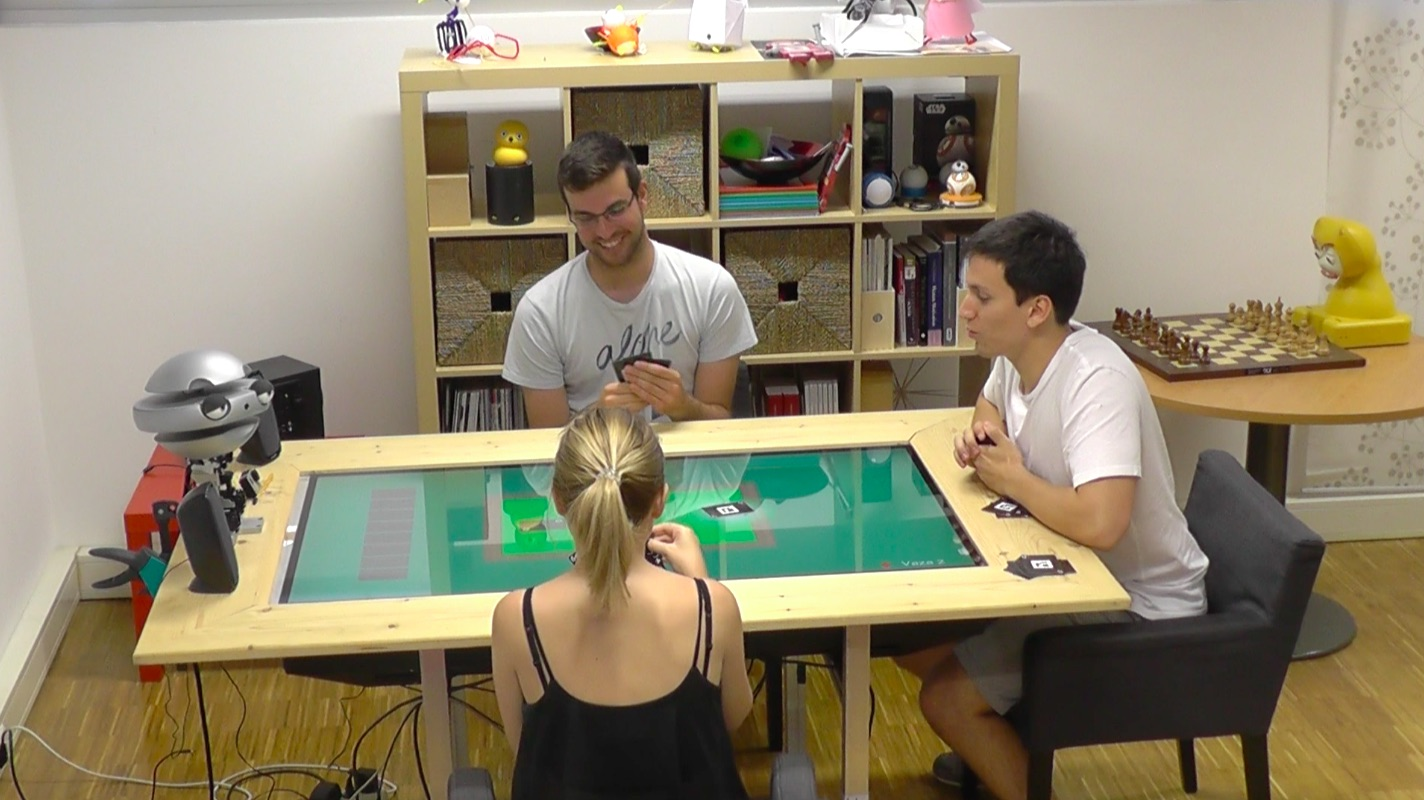
\includegraphics[width=0.7\columnwidth]{images/membership/study1}
\caption{Experimental setting for Study 1.}
\label{study1}
\end{figure}

Each participant was randomly allocated to a session in which three human participants played either with Emys or with Glin. 
This session lasted approximately 1 hour, and the instruments used were an EMYS robotic head \cite{kkedzierski2013emys}, two video cameras to record the interactions, a multi-touch table, and a deck of physical cards with printed fiducial markers that could be recognised by the table.

\subsection{Procedure}
The participants arrived at the room in groups of three. A researcher received them, explained the rules of the game, and conducted a test game to address any doubts that might arise regarding the game rules. After the explanation, the participants joined either Emys or Glin (chosen randomly) at the table and played a set of 3 games. When finished, the participants were administered a set of questionnaires, filled out the consent form and received a thank-you gift (a movie ticket). We presented the consent form at the end of the experiment so that the participants' interactions during the game would be as natural as possible. If any participant had not given consent, his or her data would have been erased. However, all participants signed the consent form.

\subsection{Measures}
To represent our sample, demographic information was requested in the questionnaires (gender, age, previous interaction with the robot and level of expertise in the game). In addition, all participants, independently of being the partner or an opponent of the robot, responded to the following questionnaires regarding the robot (Emys/Glin):

\begin{itemize}
\item \textit{Competitiveness Index} \cite{smither1992nature}, used to measure the level of competitiveness perceived in the robot. This measure is usually treated as being of a dichotomous true/false answer type; however, as our goal was to determine a range from the participants' answers, we measured it on a Likert scale ranging from ``totally disagree'' to ``totally agree''. An example of a statement would be \textit{``I consider Emys a competitive individual''} or \textit{``When Emys plays, he likes to keep an eye on the score''}.

\item \textit{McGill Friendship Questionnaire} \cite{mendelson1999measuring}, using three of its dimensions, namely, help (e.g., \textit{``Emys helps me when I need it.''}), motivation (e.g., \textit{``Emys praises me when I do something right.''}) and emotional security (e.g., \textit{``If I was worried, Emys would make me feel better''}), with scales ranging from ``totally disagree'' to ``totally agree''.

\item \textit{Relationship Assessment Scale} \cite{hendrick1988generic}, a\-dapted to the context and used to ascertain the level of quality of the relationship with the robot, ranging from ``few'' to ``a lot'' (e.g., \textit{``How good was Emys relationship with the players?''}).

\item \textit{Godspeed Questionnaire} \cite{bartneck2009measurement}, using the two dimensions of perceived intelligence and likeability to assess the level of intelligence thought to be given to the robot and its perceived likeability, measured as a semantic differential.
\end{itemize}
All dimensions were measured on a 6-point Likert scale, and when necessary, items were shuffled to mask their dimensions.

\subsection{Results}
To understand whether the two characters were perceived differently, statistical analyses were performed. When a normal distribution was present, we performed the Student's t-test for independent samples, and when the normality assumption was not met, we used the Mann-Whitney U test. The means and standard deviations are presented in Table~\ref{results-study-1}.

For the \textit{Competitiveness Index}, Emys was rated higher than Glin, with a statistically significant difference ($t(25) = -4.893$, $p<.001$).
Notably, Glin also presented a certain level of competitiveness, which was expected since it also had the goal of winning the game.
Regarding the \textit{McGill Friendship Questionnaire}, there were statistically significant differences in the three measured dimensions of help ($t(28)=2.312$, $p=.028$), motivation ($t(28)=3.686$, $p=.001$), and emotional security ($t(28)=3.218$, $p=.003$), with Glin presenting higher scores than Emys.
On the \textit{Relationship Assessment Scale}, Glin was rated higher than Emys, with a statistically significant difference ($t(28)=5.514$, $p<.001$).

These results confirm that the behavioural manipulation of the goal orientations of both robots was perceived as intended: Emys was seen as more competitive, and Glin was seen as more relationship-driven, with a greater capacity to be helpful and motivating and the ability to provide more emotional security. Moreover, the relationship quality scores were also higher for Glin than for Emys. We additionally evaluated whether the roles of the participants (partner/opponent) had any influence on the scores given to the robots, and we found no statistical significance for all measures, suggesting that the role did not affect the evaluations.

Finally, concerning the findings of the \textit{Godspeed Questionnaire}, there was no significant difference between the two robots in the perceived intelligence dimension ($t(28)=1.511$, $p=.142$). This was somewhat expected since we equipped both robots with the same algorithm for solving the card game. Although the game includes an element of chance and each new game presents different winning probabilities for each team, we can conclude that the intelligence levels of both robots were similarly perceived. However, in the likeability dimension, we found a significant difference, with Glin receiving higher scores than Emys ($U=40.50$, $p=.002$).

\begin{table}[ht]
    \renewcommand{\arraystretch}{1.2}
    \centering
    \footnotesize
    \caption{Means and ranks with standard deviations for the questionnaire dimensions comparing the evaluations of the Emys and Glin characters in Study 1. \bf*$p \leq 0.05$}.%
    \begin{tabular}{l@{}l@{} | r@{ }c@{}r@{ }|r@{ }c@{}r@{ }}
    \hline
    \multicolumn{2}{c|}{\begin{tabular}{@{}c@{}}\bf Questionnaire \\ \bf dimensions\end{tabular}} 
    & \multicolumn{3}{c|}{\bf Emys}
    & \multicolumn{3}{c}{\bf Glin} \\
    \hline
    \multicolumn{2}{c|}{Competitiveness Index \bf*} 			& $4.57$ & $\pm$ & $0.40$ & 	$3.86$ & $\pm$ & $0.33$ \\
    \hdashline
    \parbox[t]{2mm}{\multirow{3}{*}{\rotatebox[origin=c]{90}{McGill}}}
    & Help \bf*     	& $3.78$ & $\pm$ & $0.89$ & 	$4.51$ & $\pm$ & $0.81$ \\
    & Motivation \bf*   & $3.79$ & $\pm$ & $1.00$ & 	$4.95$ & $\pm$ & $0.69$ \\
    & Emo. Security \bf*& $3.26$ & $\pm$ & $1.09$ & 	$4.37$ & $\pm$ & $0.77$ \\
    \hdashline
    \multicolumn{2}{c|}{Relationship Quality \bf*} 	& $4.41$ & $\pm$ & $0.52$ & 	$5.32$ & $\pm$ & $0.38$ \\
    \hdashline
    \parbox[t]{15pt}{\multirow{4}{*}{\rotatebox[origin=c]{90}{Godspeed}}}
    & & & & & & & \\
    & Perc. Intellig.   & $4.59$ & $\pm$ & $0.74$ & 	$4.93$ & $\pm$ & $0.49$ \\
    & Likeability \bf*	& $10.70$ & $\pm$ & $0.88$ & 	$20.30$ & $\pm$ & $0.88$ \\
    & & & & & & & \\
    \hline
    \end{tabular}
    \label{results-study-1}
\end{table}


In general, it seems that our implementation was perceived by the participants as intended, and Glin was  rated as more likeable than Emys. We could now move on to the implementation of both characters at the same time, using the two robots to test which would be the preferred partner. 


\section{Study 2: Choosing a Robotic Partner}
\label{sec:study2}
The purpose of this study was to assess the participants' preferences regarding the choice of a robotic partner. 

\subsection{Sample}
For the second study, we recruited a new sample consisting of a total of 61 participants (59 university students and 2 workers), 38 male and 23 female, with ages ranging from 17 to 32 years old ($M=23.66$, $SD=3.24$). The majority of the participants had never interacted with a robot before and had a moderate or high level of expertise in the game.

We measured the level of competitiveness of each participant using the Competitiveness Index \cite{smither1992nature}: 15 participants presented low levels of competitiveness (less than or equal to $M=3.50$), 36 participants presented some level of competitiveness, and 10 participants showed high levels of competitiveness (higher than $M=4.50$).


Each session was run with two human participants who did not know each other beforehand. We controlled for this factor to ensure that the participants were in the same position with respect to both each other and the robots.
Each session lasted approximately 1 h 30 m, and the instruments used were the same as in the previous study except that two EMYS robotic heads were used simultaneously during the game interaction. A name tag was placed below each robot with its name, Emys or Glin, to allow the participants to easily identify them.


\subsection{Procedure}
The participants arrived at the room and responded to the first part of the questionnaire (see the Measures subsection below). Then, a researcher explained the game rules and conducted a test game to address any doubts that might arise. 
This study was divided into 3 consecutive sessions, as shown in Figure~\ref{3sessions-setup}.



\begin{figure}[ht]
\centering
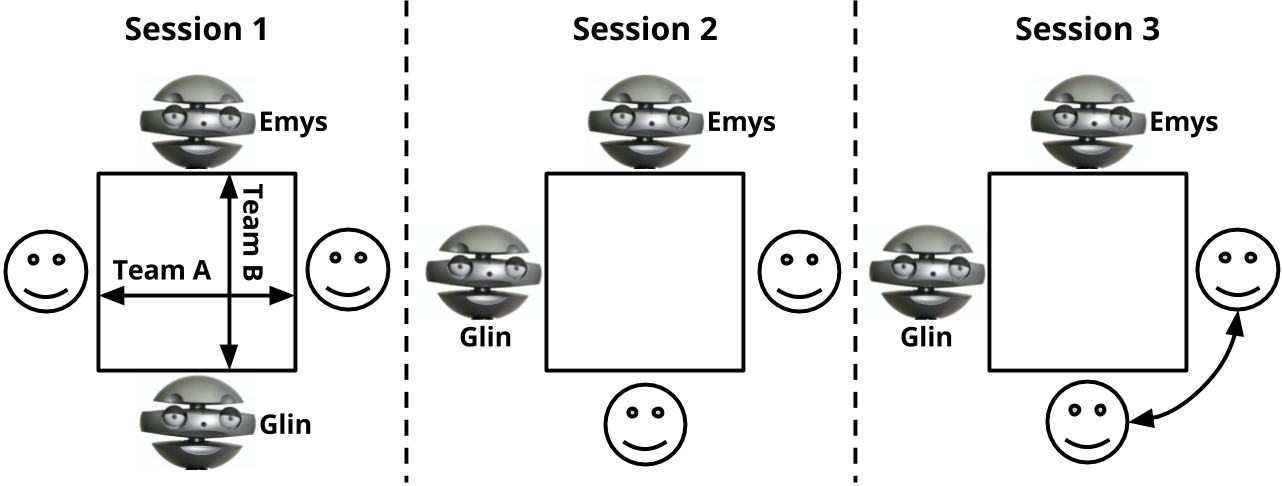
\includegraphics[width=0.9\columnwidth]{images/membership/2EmysSetUp}
\caption{Experimental setting for Study 2.}
\label{3sessions-setup}
\end{figure}

\textbf{1st Session}: The two participants partnered with each other and played a set of 3 games against the two robots (Emys and Glin), which acted as their opponents in the game. This session served to expose the participants to the two different characters while having the same role towards each one. After completion, the participants responded to the second part of the questionnaire.

\textbf{2nd Session}: Each participant partnered with one of the robots (see Fig.~\ref{study2-session2-3}), and the group played another set of 3 games. The participants then responded to the third part of the questionnaire.

\textbf{3rd Session}: The participants played their last set of 3 games, now partnering with the robots with which they had not played before, and then responded to the fourth part of the questionnaire. At the end, they were given the consent form and were thanked for their participation with a movie ticket.

The balance between the orderings was ensured by the fact that participants attended in pairs and that while one participant was Glin's partner, the other one was Emys' partner. In the last two sessions of each experiment, the participants had the opportunity to partner with both robots. We randomised which participant partnered with each robot first.

\begin{figure}[ht]
\centering
 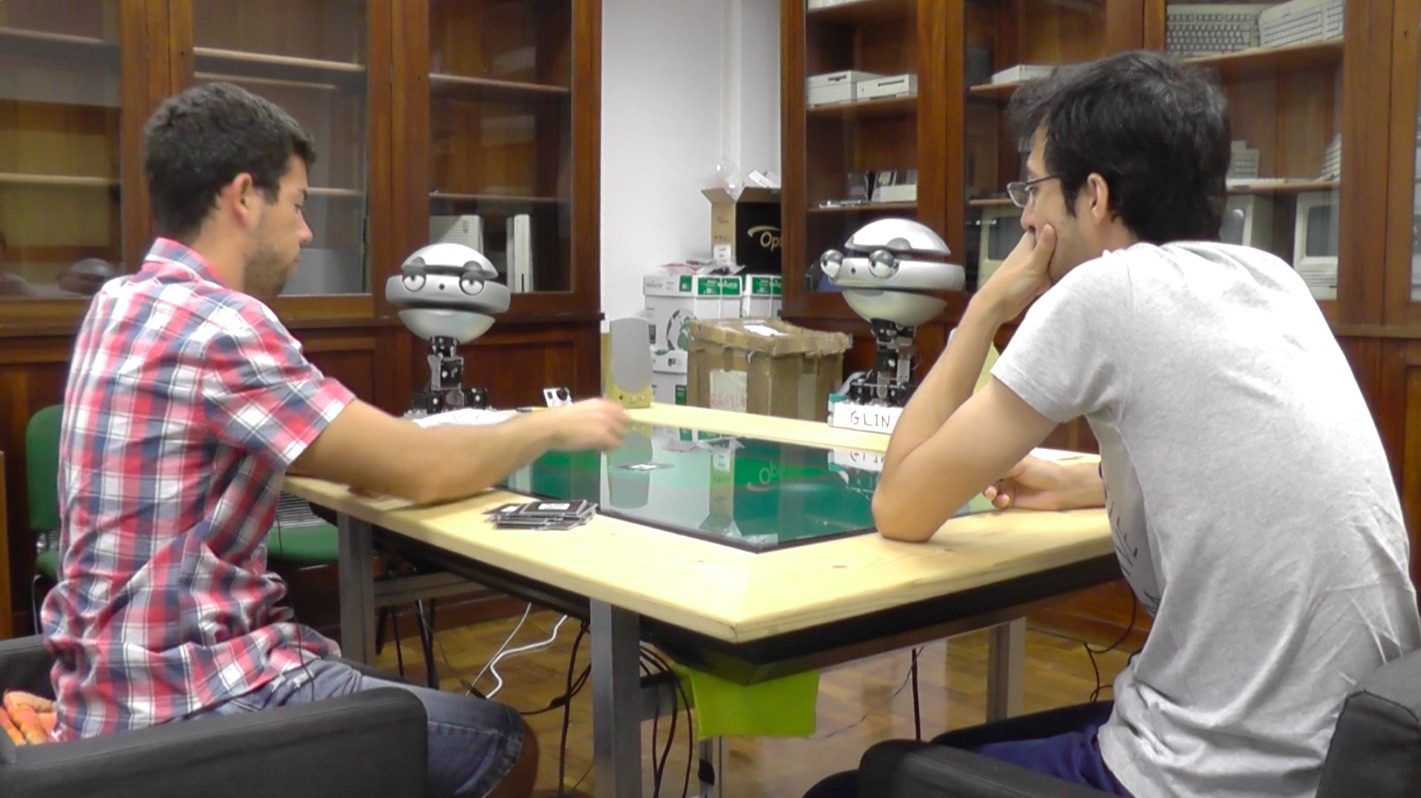
\includegraphics[width=0.7\columnwidth]{images/membership/study2}
\caption{Experimental setting for Study 2 when each robot was partnering with a human.}
 \label{study2-session2-3}
\end{figure}


\subsection{Measures}
We used the same questionnaires as in the first study, organised in the following way:

\textbf{First Part}: The participants filled out some demographic questions and then an assessment of the \textit{Competitiveness Index} related to themselves.

\textbf{Second Part}: The participants completed a questionnaire assessing the two \textit{Godspeed} dimensions (perceived intelligence and likeability) for both robots and answered the following question: ``If you could choose one of the robots as your partner, which one would it be? (Emys or Glin)''.

\textbf{Third Part}: Each participant completed a questionnaire assessing the two \textit{Godspeed} dimensions, the three \textit{McGill Friendship} dimensions (help, motivation and emotional security) and the \textit{Relationship Assessment Scale} with respect to the robot he or she had just partnered with.

\textbf{Fourth Part}: The same as the third part of the questionnaire but with respect to the new robotic partner. At the end, the participants were again asked to choose which robot they would prefer to be partnered with for future games and to justify their choice.

All dimensions were measured on a 6-point Likert scale, and when necessary, items were shuffled to mask their dimensions.

\subsection{Results}
Below, we present the results of this user study, beginning with how participants perceived each robot. Although we previously checked our manipulation, we repeated the analysis to check if the robots were perceived differently in the new 2-robot and 2-human players setting.

Then, we present the results of the participants' initial choice for the preferred robotic partner. We analysed the effect of participants' competitiveness index on this choice.

Finally, we present the participants' last choice after interacting with both robots. We analysed the effect of other measures, such as participants' competitiveness index and the team performance. We also explored changes from the initial to the last choice and the participants' justifications for the chosen partner.

Due to the high number of statistical tests performed, we performed a Holm's sequential Bonferroni correction \cite{holm1979simple} to ensure that there were no false positives in our results, and this assumption was met for all the statistical tests.




\subsubsection{Results (I) - Perception of the Robots}

We began by analysing how the participants perceived each robot in their initial interactions. When the normality assumption was not met with the Shapiro-Wilk test, we used the Wilcoxon signed-rank test. The means and standard deviations are presented in Table~\ref{results-study-2}.


Regarding the \textit{McGill Friendship Questionnaire}, the\-re were statistically significant differences in the help ($Z=-5.223$, $p<.001$), motivation ($Z=-6.066$, $p<.001$) and emotional security ($Z=-5.837$, $p<.001$) dimensions, with Glin being rated higher than Emys.
For the \textit{Relationship Assessment Scale}, there was also a statistically significant difference ($Z=-4.392$, $p<.001$), with Glin being rated higher than Emys, representing a higher relationship quality. 

These latter two results confirm the successful behavioural manipulation of the robots. After interacting with both robots, the participants seemed to perceive Glin as having a greater capacity for being helpful and motivating and for providing more emotional security compared with Emys. Moreover, the participants perceived Glin as displaying a better relationship quality than Emys.
Overall, these results seem to support the more relationship-driven characteristic with which we attempted to endow Glin, demonstrating the successful development and implementation of the two autonomous robots. 


The participants assessed the two dimensions of the \textit{Godspeed Questionnaire} for each robot twice, the first time before partnering with either of the robots and having only observed them as opponents and the second time immediately after having partnered with that robot. 
For the perceived intelligence dimension, we found no statistically significant difference between Glin and Emys in either the first measurement instance ($Z=-.733$, $p=.464$) or the second ($Z=-1.491$, $p=.136$). Thus, by using the same decision-making algorithm for both robots in this hidden-information card game, we achieved similar levels of perceived intelligence in both, as intended.
For the likeability dimension, there was a statistically significant difference, with Glin receiving higher scores than Emys in both the first measurement instance ($Z=-3.451$, $p=.001$) and the second ($Z=-6.224$, $p<.001$).



\begin{table}[ht]
    \renewcommand{\arraystretch}{1.2}
    \centering
    \footnotesize
    \caption{Means and ranks with standard deviations for the questionnaire dimensions comparing the characters Emys and Glin in Study 2. BP stands for ``before partnering'', and AP stands for ``after partnering''. \textbf{*}$p \leq 0.05$}%
    \begin{tabular}{l@{}l@{} | r@{ }c@{}r@{ }|r@{ }c@{}r@{ }}
    \hline
    \multicolumn{2}{c|}{\begin{tabular}{@{}c@{}}\bf Questionnaire \\ \bf dimensions\end{tabular}} 
    & \multicolumn{3}{c|}{\bf Emys}
    & \multicolumn{3}{c}{\bf Glin} \\
    \hline
    \parbox[t]{2mm}{\multirow{3}{*}{\rotatebox[origin=c]{90}{McGill}}}
    & Help \bf*     	& $3.35$ & $\pm$ & $1.08$ & 	$4.42$ & $\pm$ & $1.13$ \\
    & Motivation \bf*   & $3.15$ & $\pm$ & $1.09$ & 	$4.79$ & $\pm$ & $0.90$ \\
    & Emo. Security \bf*& $2.58$ & $\pm$ & $1.14$ & 	$4.29$ & $\pm$ & $1.19$ \\
    \hline
    \multicolumn{2}{c|}{Relationship Quality \bf*} 	& $3.93$ & $\pm$ & $0.89$ & 	$4.80$ & $\pm$ & $0.93$ \\
    \hline
    \parbox[t]{15pt}{\multirow{4}{*}{\rotatebox[origin=c]{90}{Godspeed}}}
    & Perc. Intellig. (BP)  & $4.51$ & $\pm$ & $0.86$ & 	$4.53$ & $\pm$ & $0.99$ \\
    & Likeability (BP) \bf*	& $3.70$ & $\pm$ & $1.19$ & 	$4.28$ & $\pm$ & $0.94$ \\
    & Perc. Intellig. (AP)  & $4.40$ & $\pm$ & $1.04$ & 	$4.55$ & $\pm$ & $1.13$ \\
    & Likeability (AP) \bf*	& $3.51$ & $\pm$ & $1.35$ & 	$5.25$ & $\pm$ & $0.75$ \\
    \hline
    \end{tabular}
    \label{results-study-2}
\end{table}



\subsubsection{Results (II) - Initial Choice of Robotic Partner}
The participants were asked to choose which robot they would like to have as a partner immediately after the first session (in which they had both robots as opponents and had partnered only with another human participant). This allowed us to assess the first impressions people had of the robots and how these would guide their choice of partner. The results showed that 38 of the participants would prefer to have Glin as a partner, whereas 22 preferred Emys. Running a chi-square goodness of fit test, we found a statistically significant difference between the participants' choices (${\chi^2}(1)=4.267$, $p=.039$), with more people preferring Glin (63.3\%) compared with Emys (36.7\%). In this stage of the experiment, the robots were on the same team, and as such, the performance of one robot could not be contrasted with the performance of the other. 
To better understand the participants' choices, we also compared the participants' competitiveness scores based on their chosen robots using the Student's t-test for independent samples, and we found that there was no statistically significant difference between the competitiveness scores of participants who chose Glin and those who chose Emys ($t(58)=1.242$, $p=.219$). This suggests that at this stage, competitiveness did not influence the partnering choice.
Therefore, the participants' choices seem to have been guided by the different social behaviours exhibited; in this case, the participants were more drawn to the relational robot (Glin), which, according to the Results (I) section, was perceived as more likeable than Emys. Thus, the findings support our hypothesis that people seem to prefer a friendlier and more relationship-oriented robotic partner.
However, we also wished to investigate whether these characteristics would continue to drive the participants' preferences after they had interacted with both robots as partners.


\subsubsection{Results (III) - Final Choice of Robotic Partner}
When asked to choose a robotic partner in the last questionnaire session (after having partnered with both robots), 35 of the participants preferred Glin and 25 preferred Emys (one participant refrained from choosing).
Running a chi-square goodness of fit test, we found no statistically significant difference between the participants' choices (${\chi^2}(1)=1.667$, $p=.197$).
We then investigated the factors driving the participants' choices at this stage of the interaction.

Looking at the levels of competitiveness of the participants and comparing them according to their final choices, we found a statistically significant difference ($t(58)=2.953$, $p=.005$), indicating that the participants who chose Emys also tended to have higher competitiveness scores ($M=4.21$, $SD=0.67$) compared with the scores of the participants who chose Glin ($M=3.73$, $SD=0.58$). This implies that a participant's own characteristics (being more or less competitive) played a role in his or her choice of robotic partner after interacting with each robot on his or her team over repeated interactions.

Since the participants partnered with both robots, we also considered the possibility that the performance of the team formed with each robot (winning or losing) also affected the partner choice. To investigate this, we calculated the performance of each human-robot team using the summed results of the sessions, i.e., the sum of the points that Glin's team earned in Session 2 + Session 3, independently of its human partners, compared with the points earned by Emys' team. We observed that based on this criterion, Emys' team won 16 times and Glin's team won 12 times (4 draws occurred). Although this difference was not statistically significant (${\chi^2}(1)=.571$, $p=.450$), we found a significant association with the partnering preference using Fisher's exact test ($p=.008$). It seems that the participants aligned their choices with the robot that was winning more. However, we must be careful with this assumption; each robot was always playing on a team, so if a particular robot won, its win was due not only to its own performance but also to its human partner's performance. Therefore, we can speak of the team performance as a factor influencing the partner choice.

Looking only at the participants who changed their choices of robotic partner between the first session and the last, we found a statistical association between the last chosen robot and that robot's team performance according to Fisher's exact test ($p=.002$). By contrast, for the participants whose choices did not change, no significant association was found according to Fisher's exact test ($p=.409$). This suggests that the participants who changed their choices did so because of the robot's team performance,
thereby solidifying the conclusion that the team performance was indeed one factor accounting for the partner choice, but not the only one.
 
To clarify whether the robot's character had any influence on the participants' choices at this stage, we analysed their justifications for preferring their chosen robots. For this purpose, two coders (who were completely unaware of the purpose of the study) coded the participants' phrases according to the following coding scheme: they coded a response as \textit{relational} if the justification for the choice of robot was more closely related to team spirit or the robot showing a warmer, more motivating, or more supportive attitude toward its partner, and they coded a response as \textit{competitive} if the justification was based on the robot being the best robot, earning more points, or being more competitive either on its own or towards its opponents. This coding scheme was based on the development objectives for the two different characters. The Cohen's kappa value was k=.73 ($p<.001$), revealing good agreement between the coders. We found from the analysis that Glin was chosen 26 times with relational justifications and only 9 times with competitive justifications. By contrast, Emys was chosen 21 times with competitive justifications and 4 times with relational justifications. 
These results suggest that the robots' characters were also perceived by the participants and used to justify their choice, although this was not the only factor considered.

Overall, these results suggest that \textit{team performance}, a \textit{person's level of competitiveness}, and the \textit{robot's character} play a role in a person's choice of a robotic partner after having previously partnered with it.


\section{Concluding Remarks}
We explored preferences regarding robotic partners in mixed teams of humans and robots. Moreover, we studied the factors driving the human participants' partnering choices. For this purpose, we developed two autonomous social robots with different characters, i.e., Emys and Glin, a more competitive robot and a more relational robot, respectively. These two autonomous robots interacted in a group with two humans while playing a competitive game. We began by validating that the two robotic characters were, in fact, differently perceived by the participants. Then, we investigated which of them would be chosen by the parti\-cipants as a partner for future games. 
The participants were asked which robotic character (Emys or Glin) they preferred at the two following points in time: (1) before having partnered with either robot and (2) after having played with both robots as partners.

The partner choices seemed to be guided by different factors depending on the context of the participants. In the first session, when the participants had experienced both robots as opponents and had not yet created a partner relationship with either, they seemed to choose their partners based solely on character (either the relationship-driven or competitive robot). At that time, Glin, the relational robot, was the preferred partner. This finding confirms our hypothesis, consistent with the study of \cite{porter2005goal}, that teams whose members prioritise relational features are perceived more positively (e.g., reporting higher levels of supportive behaviour and higher-quality interactions).

However, at the end of the final session, when they had experienced a partner relationship with each robot, the participants' choices became less clear, calling attention to other factors that came into play.
It seems that \textit{personal characteristics} and \textit{team performance} took higher precedence when participants had experienced partner-partner relationships with the robots.
The participants seemed to be affected by their \textit{own characteristics} in their partner choices, as we observed that participants with higher levels of competitiveness tended to choose the more competitive robot (Emys), whereas the less competitive participants tended to choose Glin. 
At the same time, although both autonomous robots played the game using the same algorithm and the difference between the numbers of victories achieved by Emys' and Glin's teams was not significant, there was an association between the team performance and the chosen robot. It was observed that the change in participants' choices between the first and last sessions showed a significant association with team performance. Reinforcing this observation, the performance of the team was also a factor in the final choice of the preferred partner. The same association was not observed for the participants who maintained their choices.
In addition, the robot's character also seemed to have influenced the choice, as the participants' justifications of their choices were related to the robots' characters. For example, Glin was chosen because it was much more relational, whereas Emys was chosen because it was more competitive. 

The second user study, in particular the first session where both participants were opponents to both robotic characters, was carefully designed to expose the characters to the users on an equal footing. We note, however, that the subsequent user choices and preferences might have been different without this initial session. Moreover, our results do not explore ordering effects, which might be interesting to explore in the future.

Nevertheless, these results have important implications for the creation of robotic teammates who can adapt to their human partners' specific characteristics. Consistent with recent findings \cite{fraune2017threatening} showing that people perceive multiple robots that act and look the same as more threatening than a diverse group of robots, people's preferences also need to be considered in the creation of mixed human-robot teams. Indeed, as we move towards scenarios featuring interactions among multiple robots and multiple users, the ``diversity'' of the robots should not only be investigated but also engineered.

%\section{Human-Robot Teams}
%As demonstrated in the literature on HRI, in the future, much more complex interactions between humans and robots will exist. These interactions will need to be considered and planned in regard to the design of the robots as well as their social capabilities. Robots that are going to collaborate with humans need to be designed accordingly. Accommodating the partner in the interaction can range from security measures in terms of the material used for its body to adapting its functions to complement the human actions.


%On the other hand, when we think about contexts in which social capabilities need to be embedded in the robot, other factors seem to be important in its development. If we want to implement a game partner or an opponent (e.g., a robot in an elderly care centre or a school), other factors need to be considered, and performance alone is not enough to bring enjoyment. The user characteristics will also play a huge part in the development of a game character, e.g., should the robot adapt to each person's level of competitiveness? Additionally, when playing the role of an opponent, which characteristics should the robot have? These are interesting topics that need to be further explored to understand how robots can function alongside humans in our society and how they can help and be more enjoyable during that interaction. Moreover, other dimensions of the interaction between teams of humans and robots should also be addressed as, for instance, recent findings explore socio-emotional support and gaze behaviours \cite{oliveira2018friends}. The study presented here only explores a part of these human-robot teams, as it helps to unveil people's preferences for a partner in a competitive game.

%By unveiling the tendency of people to match the robot's characteristics with their own characteristics, we also contribute to a more general understanding of membership preferences. Such preferences are linked to the perception of coherent mixed groups of humans and robots and, therefore, to the notion of social groups. These types of groups can naturally emerge in social contexts, even in scenarios without explicit competition \cite{eyssel2012social}, and are associated with the social identity theory. Previous findings in the HRI field have indeed showed that team members with strong levels of group identification also trust more their robotic team partners \cite{correia2018group}. Therefore, the preferences people have when forming teams with robots also mirror their perception of a coherent team and may be related with stronger levels of group identification. Nevertheless, further exploration is necessary to analyse the effect of congruent characteristics, e.g., goal orientation and/or other variables, of the group members on other factors required by the broader field of human-robot collaboration, such as the group performance.
\chapter{Pro-sociality}
\label{chapter:pro-sociality}

In the previous chapter, one of the concluding remarks was the fact that humans tend to value the performance obtained by the team when they have robotic teammates. However, performance may sometimes be affected, or even damaged, by external factors, e.g., luck (such as in the card-game scenario). This consideration partially motivated our second research goal -- \textit{evaluate the impact of the team’s outcome on the collective cohesion} --, which we  discuss in the current chapter.

Additionally, we want to explore another dimension of cohesiveness, \textit{collective cohesion}. It reflects the degree of identification with the group. It is usually mentioned as the replacement of the ``I'' by the ``we'' and, when this feeling becomes stronger, it may even affect one’s actions with the collective goals taking priority over the individual ones. To investigate this question, we develop a new scenario where both the outcome could be controlled and the actions of the team members would express a degree of cooperation towards a collective goal. The scenario is called ``For The Record'', a collective risk dilemma mapped into an entertaining game, and its description is presented in Section~\ref{sec:for-the-record}.

We conducted a user study where a team constituted by two social robots and one person would play a session of ``For The Record'', as detailed in Section~\ref{sec:study3}. We manipulated not only the outcome of the game to either be a victory or a loss, but also the degree of cooperation on the two robots. This experimental set-up allowed us to investigate the following three research questions:
\begin{itemize}
    \item How do people perceive pro-social and selfish actions of robotic teammates?
    \item How can the perception of those robotic teammates be affected by the outcome of the team?
    \item Does the outcome of the team affect how humans identify with the team and trust it?
\end{itemize}

The chapter proceeds with the results of the user study in Section~\ref{sec:study3-results} and a detailed discussion of our hypotheses in Section~\ref{sec:study3-discussion}. Finally, some concluding remarks are presented in Section~\ref{sec:concluding-remarks}.

\section{For The Record}
\label{sec:for-the-record}
\textit{For The Record} is as a N-person threshold game with uncertain returns. In this game, there is a public good accessible by each team member independently of her contribution. The creation of such public good (their collective goal) requires that the sum of all contributions exceeds a threshold that is uncertain. Each player tries to maximise the collective goal by contributing to the public good. At the same time, individuals may opt to free ride on the efforts of others, while choosing to invest on their own individual goals. The game is set within an artistic context, in which players are musicians of a band. Even if framed within a specific context, this class of dilemmas is general enough to capture the non-linearity and uncertain nature of many Human collective endeavours, from group hunting to climate agreements. Introducing these type of social dilemmas in HRI, especially in group interactions, allows the analysis of pro-social collaboration and, in a more general perspective, the creation of new approaches in which robots can promote pro-sociality on humans.

The following description of \textit{For The Record} considers the artistic context attributed to the game when introduced to the players. Each musician of the band has the goal of ``maximising his/her revenue by contributing to the creation of successful albums and avoiding the collapse of the band''.

The game is composed by $R$ rounds and each round is the publication of an album on the market. Before detailing the stages of the album creation, consider that each player $j$ has two distinct skills as a musician that are quantifiable in discrete levels: the musical instrument ($li_j$), and the marketing ($lm_j$). 
The instrument skill is used during the creation of an album, where each player $j$ sequentially has to evaluate her individual performance by rolling $li_j$ dice of 6 faces. Letting $D_f(n)$ denote the result of rolling $n$ dice of $f$ faces, the value of an album sums the value of each musician's performance, according to the following expression:
\[ V_{album}=\sum_{i=1}^{N} D_6(li_j) \]
After creating each album, the market value determines whether that album succeeds or fails. The market value is calculated by rolling $n$ dice of 20 faces. Additionally, \textit{For The Record} includes two difficulty levels when publishing an album on the market, called national and international market that differ according to the following expressions:
\[V_{national\_market} = D_{20}(2)\]
\[V_{international\_market} = D_{20}(3)\]
Thereupon, each album is considered either a mega hit or a fail according to the following expression:
\[ \left\{ \begin{array}{ccl}
``Mega Hit'' & \mbox{if} & V_{album} >= V_{market}\\
``Fail'' & \mbox{if} & V_{album} < V_{market}
\end{array}\right.\]
Each round ends with the players receiving their individual revenues. The revenue is $0$ when the album has failed, however, in case of a mega hit, each player $j$ has two options: to receive a default amount of $3000$ or to use his/her marketing skill and receive according to the result of rolling $lm_j$ dice of 6 faces. This second option is only available if $lm_j > 0$.



%\begin{figure}[ht]
%    \centering
%    \includegraphics[width=0.8\columnwidth]{Images/forTheRecordMainGameplayScreenshot.png}
%    \caption{\tr{Interface of\textit{For The Record} at: (a) the level up phase, where each player chooses to upgrade the instrument (cooperate) or to upgrade the marketing (defect).}}
%    \label{fig:forTheRecordMainGameplayScreenshot}
%\end{figure}

In the beginning of each round, each player has to upgrade one of his/her skills by 1 point, between the instrument and the marketing skill. %\tr{(Figure~\ref{fig:forTheRecordMainGameplayScreenshot})}. 
On the one hand, by increasing the level of the instrument, the player can roll one more dice during the evaluation of his/her performance and, therefore, increases the likelihood of producing a successful album. On the other hand, by increasing the level of the marketing, the player can roll one more dice during the revenue collection in case of a mega hit and, therefore, increases the likelihood of maximising the individual profit. In other words, each player has to choose between to cooperate, by contributing to the collective goal, or to defect, by contributing to his/her individual goal.

Another important rule is: during the $R$ rounds, if the band achieves a limit $L$ of failed albums, the game ends and each musician loses all the accumulated revenue. This is done in order to stress the importance of collaborating.


\section{User Study}
\label{sec:study3}
We conducted a user study using the previously described \textit{For The Record} game. The number of players, $N$, was 3 and the selected setting was one human participant playing together with two robotic players on a touch screen (Figure~\ref{fig:interaction}).
Furthermore, we set the number of rounds, $R$, to 5 and the limit of failed albums, $L$, to 3. The band started to publish albums on the national market and changed to the international market on the $4^{th}$ round. The initial values for the levels of each skill were the same for all the players: 1 point in the instrument skill ($li=1$), and no points in the marketing skill ($lm=0$). Finally, players could upgrade their skills from the $2^{nd}$ round on, which means they had 4 decisions to make during the 5 rounds between improving their instrument skill (cooperate) or their marketing skill (defect).

\begin{figure}[ht]
    \centering
    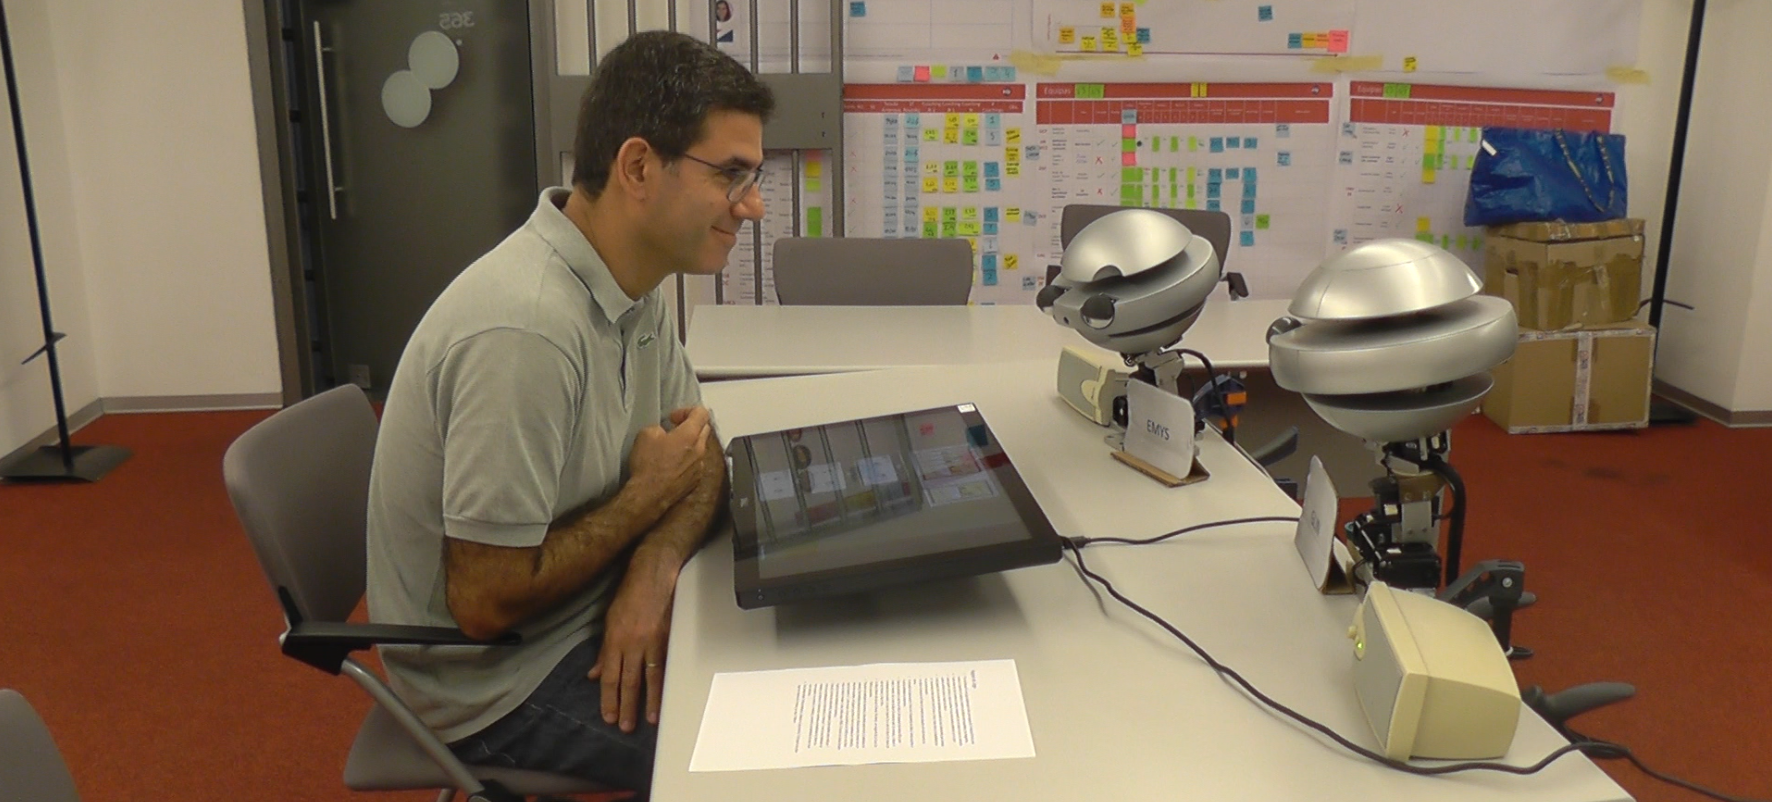
\includegraphics[width=0.7\columnwidth]{images/prosociality/interaction1.png}
    \caption{This interaction was captured during a session of the user study, where a participant is playing \textit{For The Record} game with the two robotic partners.}
    \label{fig:interaction}
\end{figure}



One particular factor that is likely to influence how people perceive their robotic teammates is whether the team succeeds or fails in the shared task. As identified in \cite{kahneman2013choices}, people are more sensitive to avoiding losses than to gains of equal monetary amount. This well-known cognitive bias is referred to as loss aversion. As a result, in this user study, we manipulated the game result in a between-subjects design, which produced two experimental conditions: winning or losing the game. In order to achieve these two deterministic outcomes, we scripted predefined orders for all the possible dice throws. Not only could we guarantee all the participants played the same number of rounds, we could also ensure that the dice rolls of the each robot were the same in both conditions. Consequently, during the 5 rounds, participants got a failure, a victory, a failure, a victory and finally either a victory or a failure according to the condition.

The robotic players differ on the strategies they apply to play the game. One of them always defects by improving its marketing skill in every round, which we call the defector, while the other always cooperates by improving its instrument skill in every round, which we call the cooperator. Nevertheless, their verbal and non-verbal behaviours remained similar and we used two versions of the same embodiment for each character, the EMYS robotic head \cite{kkedzierski2013emys}. Regarding their speech acts, they encourage the team in the beginning of each album, they comment extreme luck or bad luck on the dice rolls for both themselves and the other players and, in the end of each album, they comment the round result with an emotional animation of either sadness or joy. The three game states that were used to emphasise the difference between their distinct game strategies were:
\begin{itemize}
    \item The level up phase where each robot chooses to upgrade either its instrument skill (cooperate) or its marketing skill (defect) (e.g., Cooperator -- ``I will level up the instrument.'', Defector -- ``I will improve the marketing.'');
    \item The dice roll that corresponds to the individual performance for an album (e.g., Cooperator -- ``Wow, I added [N] points!'', Defector -- ``[N] more points for our album!'');
    \item The last decision of using or not the marketing skill to receive the revenue in case of success (e.g., Cooperator -- ``Here it comes the reward.'', Defector -- ``I will use my [N] marketing skill points to see what I can get...'').
\end{itemize}
To avoid having these autonomous robots speaking at the same time, the game engine randomly chooses which robot comments each game state. Finally, their non-verbal behaviours consists of gazing at: the other players when it is their turn; the other robot if it is speaking; or the touch screen by default.



\subsection{Hypotheses}
The following hypotheses state our expectations towards the differences on people's perceptions, judgements and preferences between a pro-social and a selfish robotic partners after teaming with them in a public goods game.
\begin{itemize}
    \item[] \textbf{H1}: The pro-social robot will be perceived more positively in its social attributes than the selfish robot.
    \item[] \textbf{H2}: The pro-social robot will be perceived as less competent than the selfish robot.
    \item[] \textbf{H3}: Group trust and group identification will be positively associated with the group performance.
    \item[] \textbf{H4}: When the team wins, the main responsible factor will be the strategy of the pro-social robot.
    \item[] \textbf{H5}: When the team loses, the main responsible factor will be the strategy of the selfish robot.
    \item[] \textbf{H6}: The pro-social robot will be preferred as a future partner, rather than the selfish robot.
\end{itemize}

Our rationale behind these hypotheses is the following. Concerning \textbf{H1} and \textbf{H6}, we expect that participants see the pro-social robot in a more positive light as it acts in a fully collaborative manner, helping the team to succeed.
The expectation behind \textbf{H2} lies in the fact that the selfish robot will always be ahead in terms of task performance (profit made). Additionally, in a study that asked participants to judge the competence of people playing the prisoner's dilemma, the results showed that those who were defected against were seen as less competent \cite{krueger2007perceptions}. It is possible that the same effect occurs in our study given that pro-social robot's behaviour. The reason for \textbf{H3} is the aforementioned loss aversion bias \cite{kahneman2013choices} and finally, \textbf{H4} and \textbf{H5} are based on the assumption that people will correctly identify the main responsible actor behind the team's result.

\subsection{Procedure}
Participation in this study was individual and started with a brief overview of each step. All the participants signed the consent form and then proceeded with the experiment. One researcher read the game rules one by one and answered participant's questions, while another researcher set up the robots and the video camera. Then, they played a training game without the robots to ensure the participant learned the game and to clarify any final doubts. The training game had a maximum of 5 rounds but the dice rolls were completely random. After that, the researcher initiated the game with the robots, alternating between conditions. Before the researchers left the room, they emphasised the goal of the study is to analyse their opinion of each robot and, therefore, they should pay attention to which is which and also to their behaviours during the game. Finally, after the interaction with the robots, each participant answered the questionnaire and was greeted by his/her participation.


\subsection{Dependent Measures}
The following dependent measures were used on the data analysis: \textbf{Competitiveness} level of the participant using a single-item question ``How competitive do you evaluate yourself?''; \textbf{Group Identification} \cite{leach2008group} using the Portuguese adaptation \cite{ramos2011adaptaccao} with the dimensions of Solidarity, Satisfaction and In-Group Homogeneity; \textbf{Group Trust} \cite{allen2004exploring}; \textbf{RoSAS} \cite{carpinella2017robotic} using its three dimensions of Warmth, Discomfort, and Competence towards each robot; \textbf{Choice of a Robotic Partner} among the defector and the cooperator for a hypothetical future game; \textbf{Responsibility (blame/credit) attribution} of four different factors -- randomness, participant's strategy, defector's strategy and cooperator's strategy -- using single-item questions ``The game result was mainly due to (...)''.
All the items in the questionnaire were assessed in a 7-points scale ranging from 1 (``Definitely not associated'') to 7 (``Definitely associated'') and the robots were always mentioned by their names.

\subsection{Sample}
The study was conducted at a company facility in order to collect a varied sample in terms of age, gender and background. There was a total of 70 participants (35 per experimental condition) with ages ranging from 22 to 63 ($M=34.6, SD=11.557$). Regarding gender, there were 32 females, 37 male, and 1 unknown.


\section{Results}
\label{sec:study3-results}
\subsection{Social Attributes of the Robots}
%\label{sec:rosas}
To analyse the impact of the game result on the perception of each robot, we used a Mixed analysis of variance (ANOVA) where the within-subjects factor is the robotic character and the between-subjects factor is the game result (winning or losing).

Regarding the perception of warmth, there was a significant main effect of the robotic character (Figure~\ref{fig:main-effects}, $F(1,67)=17.366, p<0.001, r=0.454$) with the cooperator being rated with higher values of warmth ($M=4.225, SD=1.090$) compared to the defector ($M=3.513, SD=0.977$). However, the main effect of the game result and the interaction between the robotic character and the game result were not statistically significant ($F(1,67)=0.028, p=0.869, r=0.020$ and $F(1,67)=0.013, p=0.908, r=0.014$, respectively).

For the social attribute of discomfort, there was a main effect of the robotic character (Figure~\ref{fig:main-effects}, $F(1,67)=30.982, p<0.001, r=0.562$), with the defector being rated with higher levels of discomfort ($M=2.895, SD=1.302$) than the cooperator ($M=1.895, SD=1.064$). Again, we have not found a significant main effect of the game result nor a significant interaction between the robotic character and the game result ($F(1,67)=0.525, p=0.471, r=0.088$ and $F(1,67)=1.141, p=0.289, r=0.129$, respectively).


\begin{figure}[ht]
\centering
%%% PLOT FILE - Perceptions of the robots - main effect of the robot on warmth and discomfort
\begin{tikzpicture}%
\begin{axis}[%
    ybar,%
    %title=Test,%
    axis y line*=left, axis x line*=bottom,%
    ymin=0,
    ymax=7.5,
    ytick={1,2,...,7},
    legend style={at={(1.4,1)}},
    %x tick label style={rotate=45,anchor=east},%
    symbolic x coords={Warmth,Discomfort},%
    xtick=data,
    enlarge x limits=1,
    bar width=15pt,
    height=5.5cm,
    %ylabel=difference in \%,%
        ]%
\addplot+[
    color=black, %
    fill={rgb,255:red,173; green,192; blue,202},%
    %postaction={pattern=crosshatch dots},
    error bars, y dir=both, y explicit]
				coordinates {
				(Warmth,4.22) +- (Warmth,0.264)
				(Discomfort,1.89) +- (Discomfort,0.258)};
\addplot+[%
    color=black, %
    fill={rgb,255:red,87; green,87; blue,94},%
    error bars/.cd,%
    y dir=both,%
    y explicit,%
        ]%
coordinates {
            (Warmth,3.50) +- (Warmth,0.236)
            (Discomfort,2.92) +- (Discomfort,0.31)
        };%
    
\draw (axis cs:Warmth,6.5) ++ (-10pt,0pt) -- ++(20pt,0pt);
\node[anchor=south] at (axis cs:Warmth,6.5) {***};
    
\draw (axis cs:Discomfort,6.5) ++ (-10pt,0pt) -- ++(20pt,0pt);
\node[anchor=south] at (axis cs:Discomfort,6.5) {***};

\legend{Cooperator,Defector}
\end{axis}%
\end{tikzpicture}%
\caption{Main effect of the robotic partner on the social attributes of warmth and discomfort.}
\label{fig:main-effects}
\end{figure}

These results suggest that the distinct strategies adopted by the robots affected the perception of the robot's warmth and the discomfort they felt regardless of the game result.

In terms of the perception of competence, there was a significant main effect of the robotic character ($F(1,67)=24.873, p<0.001, r=0.520$), with the the cooperator being rated with higher levels of competence ($M=4.790, SD=1.111$) than the defector ($M=3.907, SD=1.073$). Although we did not find a significant effect of the game result ($F(1,67)=0.966, p=0.329, r=0.119$), there was a significant interaction between the robotic character and the game result (Figure~\ref{fig:interaction-effect}, $F(1,67)=4.095, p=0.047, r=0.240$). To understand this interaction, we compared the perception of competence attributed to each robot across the two possible game results using a Wilcoxon Signed-Rank test. In the case where the game result was winning, there was no significant difference between the competence attributed to each robot ($Z=-1.859, p=0.063, r=-0.319$). However, in the case where the game result was losing, there was a significant difference between the competence attributed to each robot ($Z=-4.434, p<0.001, r=-0.749$), with the cooperator being rated as more competent ($M=4.876, SD=0.958$) than the defector ($M=3.624, SD=0.896$).


\begin{figure}[ht]
\centering
%%% PLOT FILE - Perceptions of the robots - interaction effect on competence between robot and condition
\begin{tikzpicture}%
\begin{axis}[%
    %ybar,%
    %title=Test,%
    axis y line*=left, axis x line*=bottom,%
    ymin=0,
    ymax=7.5,
    ytick={1,2,...,7},
    legend style={at={(1.4,1)}},
    %x tick label style={rotate=45,anchor=east},%
    symbolic x coords={Winning,Losing},%
    xtick=data,
    enlarge x limits=1,
    bar width=15pt,
    height=5.5cm,
    %ylabel=difference in \%,%
        ]%
\addplot+[
    color=black, %
    %mark size=4pt,
    mark options={
    fill={rgb,255:red,173; green,192; blue,202},%
    },
    error bars, y dir=both, y explicit]
				coordinates {
				(Winning,4.70) +- (Winning,0.382)
				(Losing,4.88) +- (Losing,0.376)};
\addplot+[%
    color=black, %
    mark size=2pt,
    mark options={
    fill={rgb,255:red,87; green,87; blue,94},%
    },
    error bars/.cd,%
    y dir=both,%
    y explicit,%
        ]%
coordinates {
            (Winning,4.17) +- (Winning,0.358)
            (Losing,3.62) +- (Losing,0.353)
        };%


\draw (axis cs:Losing,4.25) ++ (10pt,-10pt) -- ++(0pt,20pt);
\node[anchor=south] at (140,380) {***};

%\draw (axis cs:Winning,4.4) ++ (-10pt,-10pt) -- ++(0pt,20pt);
%\node[anchor=south] at (-30,410) {n.s.};

\legend{Cooperator,Defector}
\end{axis}%
\end{tikzpicture}%
\caption{Interaction effect between the robotic partner and game result on the attributed levels of competence.}
\label{fig:interaction-effect}
\end{figure}

Contrary to the previous social attributes, the competence attributed to each robot was affected by the game result. Participants have considered the cooperator as more competent only in the losing condition. This result suggests the negative effect of losing the game highlighted the difference in perceived competence between the robots.

\subsection{Group Measures}

To analyse the two dependent measures related to the group (Figure~\ref{fig:group}), i.e. group identification and group trust, between the two possible game results, we used Mann-Whitney U tests. Results showed a significant difference between the levels of group identification according to the condition ($U=404.5, Z=-2.445, p=0.014, r=-0.292$), with participants that won the game reporting higher levels of group identification ($M=4.267, SD=1.346$) than participants who have lost the game ($M=3.466, SD=1.182$). Nevertheless, there was no significant difference between the levels of group trust according to the game result ($U=535.5, Z=-0.715, p=0.474, r=-0.086$).


\begin{figure}[ht]
\centering
%%% PLOT FILE - Group measures condition
\begin{tikzpicture}%
\begin{axis}[%
    ybar,
    %title=Test,%
    axis y line*=left, axis x line*=bottom,%
    ymin=0,
    ymax=7.5,
    ytick={1,2,...,7},
    legend style={at={(1.4,1)}},
    %x tick label style={rotate=45,anchor=east},%
    symbolic x coords={G. Identification,Trust},%
    xtick=data,
    enlarge x limits=1,
    bar width=15pt,
    height=5.5cm,
    %ylabel=difference in \%,%
        ]%
\addplot+[%
    color=black, %
    fill={rgb,255:red,39; green,100; blue,123},%
    %postaction={pattern= north east lines},
    error bars/.cd,%
    y dir=both,%
    y explicit,%
        ]%
coordinates {
            (G. Identification,4.22) +- (G. Identification,0.464)
            (Trust,3.98) +- (Trust,0.365)
        };%
\addplot+[
    color=black,
    fill={rgb,255:red,202; green,53; blue,66},%
    error bars, y dir=both, y explicit]
				coordinates {
				(G. Identification,3.47) +- (G. Identification,0.407)
				(Trust,3.79) +- (Trust,0.291)};
    
\draw (axis cs:G. Identification,6.5) ++ (-10pt,0pt) -- ++(20pt,0pt);
\node[anchor=south] at (axis cs:G. Identification,6.5) {*};

\legend{Winning,Losing}
\end{axis}%
\end{tikzpicture}%
\caption{Effect of the game result on the attributed levels of group identification and group trust.}
\label{fig:group}
\end{figure}

These results revealed the group identification was affected by the game result, winning or losing the game, as we have predicted. However, the prediction about the measure of group trust was not confirmed, suggesting that other factors might have contributed to this outcome. Therefore, we conducted an additional analysis to interpret these surprising findings, by creating predictive models of both the group identification and the group trust levels. We used Stepwise regressions with the backward method to determine which variables could explain most of the variance of group identification and group trust levels. The initial seven predictor variables were the ones related with individual and group perceptions of the team members: defector's warmth, defector's competence, defector's discomfort, cooperator's warmth, cooperator's competence, cooperator's discomfort, and either group identification or group trust.

Regarding the group identification level, % (Table~\ref{tab:group-id-reg}), 
we found in the $5^{th}$ step that it can be significantly predicted ($F(3,65)=33.016, p<0.001, R^2=0.604$) by - $1.652$ + $0.843$ (group trust) + $0.375$ (defector's competence) + $0.158$ (cooperator's competence), where variables are assessed with 7-points likert scales. %The remaining possible predictors were excluded according to the removal criterion of not making a significant contribution to the model, respectively: defector's warmth ($t(2)=-0.179, p=0.859$) in $1^{st}$ step ($F(7,61)=14.294, p<0.001, R^2=0.621$); cooperator's warmth ($t(2)=0.252, p=0.802$) in $2^{nd}$ step ($F(6,62)=16.935, p<0.001, R^2=0.621$); defector's discomfort ($t(2)=0.475, p=0.636$) in $3^{rd}$ step ($F(5,63)=20.616, p<0.001, R^2=0.621$); and cooperator's discomfort ($t(2)=1.332, p=0.188$) in $4^{th}$ step ($F(4,64)=26.028, p<0.001, R^2=0.619$).
%\begin{table}[ht]
%\centering
%\renewcommand{\arraystretch}{1.2}
%\begin{tabular}{lccc}
 %                   & \textbf{B} & \textbf{SE B} & \textbf{$\beta$} \\ \hline
%Constant            & -1.721     & 0.673         &                  \\
%Group Trust         & 0.849      & 0.114         & 0.610            \\
%Defector's Competence   & 0.391      & 0.101         & 0.318            \\
%Cooperator's Competence & 0.159      & 0.093         & 0.134           
%\end{tabular}
%\caption{Predictive model of the group identification level at the $5^{th}$ step using the forward method.}\label{tab:group-id-reg}
%\end{table}
Regarding the prediction of the group trust level, % (Table~\ref{tab:group-trust-reg}), 
we found in the $6^{th}$ step that it can be significantly predicted ($F(2,66)=40.455, p<0.001, R^2=0.551$) by $2.513$ + $0.489$ (group identification) - $0.174$ (defector's discomfort), where variables are assessed with 7-points likert scales. %The remaining variables were excluded according to the removal criterion of not making a significant contribution to the model, respectively: defector's warmth ($t(2)=0.764, p=0.448$) in $1^{st}$ step ($F(7,61)=11.284, p<0.001, R^2=0.564$); cooperator's warmth ($t(2)=0.666, p=0.508$) in $2^{nd}$ step ($F(6,62)=13.207, p<0.001, R^2=0.561$); cooperator's discomfort ($t(2)=-0.769, p=0.445$) in $3^{rd}$ step ($F(5,63)=15.900, p<0.001, R^2=0.558$); cooperator's competence ($t(2)=-0.447, p=0.657$) in $4^{th}$ step ($F(4,64)=19.854, p<0.001, R^2=0.554$); and defector's competence ($t(2)=-1.204, p=0.233$) in $5^{th}$ step ($F(3,65)=26.735, p<0.001, R^2=0.552$).

%\begin{table}[ht]
%\centering
%\renewcommand{\arraystretch}{1.2}
%\begin{tabular}{lccc}
%                    & \textbf{B} & \textbf{SE B} & \textbf{$\beta$} \\ \hline
%Constant            & 2.487     & 0.326         &                  \\
%Group Identification         & 0.481      & 0.061         & 0.669            \\
%Defector's Discomfort & -0.160      & 0.061         & -0.220           
%\end{tabular}
%\caption{Predictive model of the group trust level at the $6^{th}$ step using the forward method.}\label{tab:group-trust-reg}
%\end{table}

This exploratory analysis allowed us to understand that although there is a correlation between group identification and group trust, they were affected by other factors, after partialling out the shared explanatory effect of the other variables. Besides the strong relation of one another, group identification can also be predicted from the competence attributed to each of the team members, and group trust can also be predicted from the discomfort attributed to the defector.

\subsection{Responsibility (Blame / Credit) Attribution}

To analyse the responsibility attribution of the game result among the following four factors of (1) randomness, (2) participant's strategy, (3) defector's strategy and (4) cooperator's strategy, we used Friedman's ANOVA tests. In the winning condition (Figure~\ref{fig:credit}), we found no significant differences on the credit attribution to the four factors ($\chi^2(3)=7.142, p=0.067, r=0.070$). However, in the losing condition (Figure~\ref{fig:blame}), the blame attribution was significantly different to the four possible factors ($\chi^2(3)=33.264, p<0.001, r=0.326$).



\begin{figure}[ht]
\centering
%%% PLOT FILE - Responsibility attribution in the winning condition
\begin{tikzpicture}%
\begin{axis}[%
    ybar,
    %title=Test,%
    axis y line*=left, axis x line*=bottom,%
    ymin=0,
    ymax=7.5,
    ytick={1,2,...,7},
    %legend style={at={(1.4,1)}},
    x tick label style={rotate=25,anchor=east},
    symbolic x coords={Randomness,Participant\textquotesingle s Strat.,Defector\textquotesingle s Strat.,Cooperator\textquotesingle s Strat.},%
    xtick=data,
    x=36pt,
    enlarge x limits=0.5,
    height=5.5cm,
    bar width=15pt,
    xticklabel style={font=\footnotesize},]%
\addplot+[
    color=black,
    fill={rgb,255:red,39; green,100; blue,123},%
    %postaction={pattern= north east lines},
    error bars, y dir=both, y explicit]
				coordinates {
				(Randomness,4.32) +- (Randomness,0.51)
				(Participant\textquotesingle s Strat.,4.91) +- (Participant\textquotesingle s Strat.,0.46)
				(Defector\textquotesingle s Strat.,3.47) +- (Defector\textquotesingle s Strat.,0.78)
				(Cooperator\textquotesingle s Strat.,4.91) +- (Cooperator\textquotesingle s Strat.,0.6)};
%\legend{Winning,Losing}
\end{axis}%
\end{tikzpicture}%
\caption{Responsibility attributed to each factor in winning condition (credit).}
\label{fig:credit}
\end{figure}

\begin{figure}[ht]
\centering
%%% PLOT FILE - Responsibility attribution in the losing condition
\begin{tikzpicture}%
\begin{axis}[%
    ybar,
    %title=Test,%
    axis y line*=left, axis x line*=bottom,%
    ymin=0,
    ymax=7.5,
    ytick={1,2,...,7},
    %legend style={at={(1.4,1)}},
    x tick label style={rotate=25,anchor=east},%
    symbolic x coords={Randomness,Participant's Strat.,Defector's Strat.,Cooperator's Strat.},%
    xtick=data,
    x=36pt,
    enlarge x limits=0.5,
    height=5.5cm,
    bar width=15pt,
    xticklabel style={font=\footnotesize}
    %ylabel=difference in \%,%
        ]%
\addplot+[
    color=black,
    fill={rgb,255:red,202; green,53; blue,66},%
    error bars, y dir=both, y explicit]
				coordinates {
				(Randomness,3.50) +- (Randomness,0.58)
				(Participant's Strat.,3.26) +- (Participant's Strat. Strat.,0.49)
				(Defector's Strat.,5.56) +- (Defector's Strat.,0.53)
				(Cooperator's Strat.,3.26) +- (Cooperator's Strat.,0.59)};
    
\addplot[black, sharp plot]%
    coordinates {(Participant's Strat.,6.3) (Defector's Strat.,6.3)}%
    node[above] at (150,610) {*};%
\addplot[black, sharp plot]%
    coordinates {(Defector's Strat.,6.6) (Cooperator's Strat.,6.6)}%
    node[above] at (250,640) {*};%
\addplot[black, sharp plot]%
    coordinates {(Randomness,6.9) (Defector's Strat.,6.9)}%
    node[above] at (100,670) {*};%
%\draw (axis cs:Participant's Strat.,6.5) ++ (-10pt,0pt) -- ++(20pt,0pt);
%\node[anchor=south] at (axis cs:Participant's Strat.,6.5) {***};
\end{axis}%
\end{tikzpicture}%
\caption{Responsibility attributed to each factor in losing condition (blame).}
\label{fig:blame}
\end{figure}


To follow up this finding on the attribution of blame, we conducted a \textit{post hoc} analysis using Wilcoxon Ranks tests. Moreover, we applied a Bonferroni correction and all the effects are reported at a $0.008$ level of significance. It appeared that all the pairwise comparisons involving the defector's strategy were significant. In the losing condition, participants attributed higher levels of blame to the defector's strategy ($M=5.429, SD=1.685$) when compared to the randomness factor ($M=3.543, SD=1.669; Z=-3.421, p<0.001, r=-0.578$), to the participant's strategy ($M= 3.265, SD=1.377; Z=-4.586, p<0.001, r=-0.786$), and to the cooperator's strategy ($M= 2.743, SD=1.669; Z=-3.909, p<0.001, r=-0.661$). Regarding the remaining pairwise comparisons, there was no significant difference between levels of blame attributed to the randomness factor and to the participant's strategy ($Z=-0.745, p=0.456, r=-0.128$), nor between the randomness factor and the cooperator's strategy ($Z=-2.201, p=0.028, r=-0.372$), nor between the participant's strategy and the cooperator's strategy ($Z=-1.284, p=0.199, r=-0.220$). These results reveal that there was no clear main responsible factor in the credit attribution of the winning outcome. However, participants clearly identified the defector's strategy as the main cause of the losing outcome.


\subsection{Choice of a Robotic Partner}

To analyse the choice of a robotic partner among the defector and the cooperator for a hypothetical future game, we used a Chi-Square Goodness-of-Fit test. Results indicated a significant difference in the preference for a robotic partner ($\chi^2(1)=22.857, p<0.001, r=0.326$), with the cooperator being preferred (55 times, $78.6$\%) to the defector (15 times, $21.4$\%).

Additionally, we found a significant association between the preferred robot and the game result ($\chi^2(1)=14.339, p<0.001, \phi_c=0.453$) and we have, therefore, also analysed preferences across conditions (Figure~\ref{fig:preferences}). In the losing condition, there was again a significant difference ($\chi^2(1)=31.114, p<0.001, r=0.889$), with the cooperator being preferred (34 times, $97.1$\%) to the defector (1 time, $2.9$\%). However, in the winning condition, no significant difference was found ($\chi^2(1)=1.400, p=0.237, r=0.040$), with the cooperator being chosen 21 times ($60.0$\%) and the defector 14 times ($40.0$\%).


\begin{figure}[ht]
\centering
%%% PLOT FILE - Choice of a robotic partner
\begin{tikzpicture}%
\begin{axis}[%
    ybar,
    %title=Test,%
    axis y line*=left, axis x line*=bottom,%
    ymin=0,
    ymax=40,
    ytick={5,10,...,35},
    legend style={at={(1.4,1)}},
    %x tick label style={rotate=45,anchor=east},%
    symbolic x coords={Winning, Losing},%
    xtick=data,
    enlarge x limits=1,
    height=5.5cm,
    bar width=15pt,
    ylabel=\# participants,%
    nodes near coords,
        ]%
\addplot+[
    color=black, %
    fill={rgb,255:red,173; green,192; blue,202},%
    %postaction={pattern=crosshatch dots},
    %error bars,
    y dir=normal,
    %y explicit
    ]
				coordinates {
            (Winning,21.0)
            (Losing,34.0)
				};
\addplot+[%
    color=black, %
    fill={rgb,255:red,87; green,87; blue,94},%
    %error bars/.cd,%
    y dir=normal,%
    %y explicit,%
        ]%
coordinates {
            (Winning,14.0)
            (Losing,1.0)
        };%
\legend{Cooperator,Defector}
\end{axis}%
\end{tikzpicture}%
\caption{Preferences for each robotic partner grouped by conditions.}
\label{fig:preferences}
\end{figure}

When breaking down the choices of the participants across conditions, their preference is only clear when they lost the game. These results suggest that the negative impact of losing the game enhances the selfishness of the defector.


%\subsection{Strategies and Impressions of the Participants}
\subsection{Strategy analysis}
We analysed the playing strategies of the participants by looking at the number of times they have defected among their 4 decisions during the game. There were 8 participants that have never defected (11.4\%), 21 that have defected once (30\%), 33 that have defected twice (47.1\%), 7 that have defected 3 times (10\%), and only 1 that always defected (1.4\%). Furthermore, out of the 33 that defected 2 times, 24 of them chose the strategy of ``cooperate, defect, cooperate, and defect''. Additionally, we found a weak positive correlation between the self-reported competitiveness level of the participants and the number of times they have defected ($r(70)=0.235, p=0.05$).

%\tmightremove{Although the profit each robot achieved during the game was scripted, the profit of the participant varies according to his decisions. We analysed the differences between the average profit that each player got, considering for the losing condition the values they have accumulated until the $4^{th}$ round. Using Friedman's ANOVA test, we found there is a significant difference between the profit of each player ($\chi^2(2)=124.427, p<0.001, r=0.889$). Moreover, all the pairwise comparisons revealed significant differences: between the profit of the defector ($M=25.000, SD=9.065$) and the profit of the participants ($Z=-7.300, p<0.001, r=-0.872; M=10.329, SD=4.442$); between the profit of the cooperator ($M=7.500, SD=1.511$) and profit of the participant ($Z=-6.104, p<0.001, r=-0.730$); and between the profit of the defector and the profit of the cooperator ($Z=-7.504, p<0.001, r=-0.897$). In other words, the pro-social robot had less profit than the others, the selfish robot had more profit than the others, and the participant had an in-between average profit.}

Finally, we did a correlation analysis to understand if the participants' perceptions of the robotic partners were associated with their competitiveness level or their playing strategy. In the winning condition, we found a moderate negative correlation between the rate of cooperation and the perceived impact of the defector’s strategy ($r=-0.379, n=34, p=0.027$) and a moderate positive correlation between the rate of cooperation and the perceived impact of the self strategy ($r=0.426, n=35, p=0.011$). No similar significant correlations were found in the losing condition. This suggests participants that cooperated more with team attributed more credit to their own strategy and less credit to the defector's strategy.

\subsection{Societal Impact}
Due to the diversity of our sample, we asked participants, at the end of the questionnaire, their agreement level on the sentence ``Social robots will be relevant to the society'', ranging between 1 (``Totally disagree'') and 7 (``Totally agree'').
Interestingly, we found a significant difference on their answers between conditions ($U=435, Z=-2.143, p=0.032, r=-0.256$), revealing a higher acceptance of social robots when they won the game ($M=5.457, SD=1.651$), compared to when they lost the game ($M=4.686, SD=1.676$).



\section{Discussion}
\label{sec:study3-discussion}
According to \textbf{H1}, we have predicted that the pro-social robot would be perceived more positively than the selfish robot. We validated this hypothesis as the cooperator was rated as warmer and caused less discomfort. Our results suggest that the display of a pro-social strategy by the robotic partner enhanced the perception of its social attributes.

We have also predicted in \textbf{H2} that the selfish robot would be perceived as more competent, which was not confirmed. In fact, the opposite result was found, although only in the losing condition. This hypothesis was based on the fact that the defector uses the optimal strategy of maximising its profit on the efforts of the others, commonly called the free rider. One possible explanation is that participants construed the notion of competence as one that necessitates the absence of exploitation of others and, therefore, even though selfish acts are highly profitable, they are deemed as incompetent. It is also the case that, in the long run with multiple iterations of the game being played, the higher return obtained by a selfish strategy will diminish when considering the results obtained for the future partner choice in the losing condition. Another possible contributing factor is that participants were highly sensitive to the risk involved in the uncertainty threshold of this game. Consequently, when participants lost the game, the evidence of a risky strategy became blameworthy and unreasonable.

Our results partially support \textbf{H3} as group identification was indeed positively associated with the performance of the group, although the same association was not verified for group trust. This surprising difference led us to analyse more carefully which factors were predicting both measures. According to our regression analysis, the best predictors of group identification were the group trust and the competence of each team member. Considering the discussion about H2, the competence attributed to the defector was significantly different across conditions. This can be the reason why there was also a significant difference on the levels of group identification.

On the other hand, the regression analysis for the group trust revealed that its best predictors were group identification (as they were highly correlated) and the discomfort attributed only to the defector. As the discomfort attributed to the defector remained similar in the two conditions, it seems to have strongly influenced the level of trust to follow the same pattern. Interestingly, literature on human-robot trust has previously suggested that performance is one of the most influencing factors to develop trust \cite{hancock2011meta}, which only occurred for group identification rather than for group trust.

Our results do not support \textbf{H4}, which predicted that, when the team wins, the main responsible factor would be the strategy used by the pro-social robot. There was no main responsible factor on the credit attribution of the winning outcome.
%\tr{We believe that according to self-serving bias \cite{you2011robot}, the tendency to attribute self-responsibility for positive outcomes might have slightly reduced the credit attribution to the pro-social robot.}
Only 8 participants (11\%) used the same pro-social strategy of cooperating 4 times and
%the mode was to defect 2 times in their 4 decisions (47\%).
most participants defected at least 2 times (58.5\%).
Although most participants were more selfish than the pro-social robot, they attributed credit similarly between their own strategy and pro-social strategy.


According to \textbf{H5}, we have predicted that when the team loses, the main responsible factor would be considered the strategy of the selfish robot. Our results supported this hypothesis as the blame attribution to selfish robot were significantly higher than all the other 3 factors: randomness, the strategy of the participant, and the strategy of the pro-social robot.


Finally, \textbf{H6} hypothesised that the pro-social robot would be preferred as a future partner, which was only partially verified from our results. The preference for the pro-social robot was only clear in the losing condition. It seems that their preferences of a future partner were aligned with the responsibility attributions they mentioned and their perceptions of competence. The negative impact of losing the game might have stressed participants' judgements, which was denoted by significant differences on this choice.%, the responsibility attribution, and the perception of competence in the losing condition.

\section{Concluding Remarks}
\label{sec:concluding-remarks}

We are moving towards a society in which robots are increasingly present and able to work with us. In this project, we explored the role of pro-sociality as a contributing factor to establish cohesive collaborations with robots and, in particular, the impact of the outcome on the establishment of those alliances.

We conducted a user study where each participant formed a team with two autonomous robots to play a public goods game. In this type of social dilemmas, players have essentially to decide between acting in a pro-social manner by opting for the collaborative goal (cooperate) or acting in a selfish manner by choosing the individual goal (defect). The two robotic players used opposite strategies during the game: the selfish robot always defected while the pro-social always cooperated. Moreover, we manipulated the outcome of the game to either result in winning or losing.

Results showed that a pro-social partner can be perceived more positively in terms of its social attributes regardless of the game result, which generally reveals the importance of group-oriented decisions by social robots.
%In this article, we introduced a game named \ftr{} which, in each round, presents to the players a public goods social dilemma. 
%% In each round of the game, players are presented with , as they must decide to either play for the benefit of the group or themselves.
%We performed experiments where each participant played a manipulated version of the game (providing either wins or losses) along with two robots who acted according to different strategies: a pro-social robot, which always cooperated and a selfish one which always decided to defect.
%After we analysed the results, we concluded that although only the outcome of the game was manipulated, more positive social attributes were assigned to the pro-social robot. In our opinion, this occurred because people gave major importance to the group-oriented decisions taken by such agent. 
Additionally, the differences between the participants' perception of competence, responsibility attribution and preferred robot were only significant when the participants lost the game. In particular, the portrayal of selfish behaviours by a robotic partner was negatively identified only when the performance of the team was compromised. More broadly, loosing outcomes seem to increase the people's awareness of what decisions players took throughout the game, and what impacts such decisions have for the success of the group.


This project also shed some light on the development of trust and group identification towards mixed human-robot teams. In fact, many authors working on this topic have focused on trust, given that it is a critical element for group collaboration. Interestingly, in this study we found that the success of the team produced an increase in group identification but not in group trust. This has a broad implication that suggests these two measures can vary independently of one another. Furthermore, we provided some evidence on which social attributes of a robotic team member play a role on the levels of trust and group identification. These findings contribute not only to the understanding of these measures, but also to enhance human-robot collaboration.
% Bullets are not welcome and to extensive ;)
% Several important conclusions were taken from the experiment results: 
% \begin{itemize}
%     \item 
%     The display of a pro-social strategy in this kind of scenarios is well received by people (social attributes like warmth, discomfort and competence were more positively perceived when participants described their views of the cooperative robot);
%     \item 
%     Against our expectations, when loosing a game, people perceived the cooperative robot as being more competent, which we believe occurred because big attention was given to the risk implied by the defector's actions;
%     \item
%     Although, as we predicted, group identification was correlated with the performance of the group, surprisingly the same was not observed for group trust. We concluded that the first correlation was due to the differences seen on the competence perceptions of both robots. On the other hand, we have seen that the relevant best predictor for group trust was the discomfort attributed to the defector, which did not change if the game was either won or lost;
%     \item
%     Opposite to our expectations, the cooperator was not perceived as being responsible for the won games. This fact might be due to the phenomena of self-driving bias. However, when the team lost, the defector was blamed as expected;
%     \item
%     Finally, only when loosing the game did people chose the cooperator as a future partner. We think the negative impact of a loss might have been the cause of such occurrence.
% \end{itemize}

Finally, an important consideration of our user study was the fact it took place at the facility of a large company and, therefore, our sample is more balanced in terms of ages and backgrounds than the most commonly reported  samples that consist of young adults from universities \cite{baxter2016characterising}. 


%As future work, it would be interesting to analyse the influence of the embodiment on the current findings, by replicating this user study with non-embodied agents.
%%As future work, it would be interesting to check if the presented results can be replicated when using non-embodied agents. In other words, we can observe if the use of pure virtual agents acting like our robots provides the same conclusions.
%We would also like to explore the ingroup/outgroup relations of humans and robots, similar to what was done in \cite{chang2012effect, fraune2017teammates}, by for instance changing the proportion between the number of human and robotic team players.
%%In our study only one person was teamed up with two robots (the robots were the majority). However, we can check what differences might occur in people's perceptions and judgements when building groups having different humans-to-robots proportions/ sizes, for example 2 humans and 1 robot, 2 humans and 2 robots, etc.
%Another aspect we are keen to work on is the impact of using different game strategies that are neither purely pro-social nor purely selfish.
%%In fact, strategies which act according to specific states of the game are interesting to explore (for example, act cooperatively when the team is loosing and defect when the team is winning).
%Finally, it would also be interesting to analyse the inclusion of additional social mechanisms such as punishments. This could be done either by (1) approaching the notion of altruistic punishment or (2) implying punishment in the agents' social behaviours, similar to \cite{vollmer2018children}.
%%Finally, it would also be interesting to extend our analysis to other social mechanisms such as studying the effects of using punishment.
%%(punishing others at a cost: for example, giving players the ability to use their profit to punish other players)


\chapter{A model of Group-based Emotions}
\label{chapter:group-based-emotions}

% RESEARCH QUESTION can the expression of group-based emotions by a robotic teammate increase people's identification and trust with the team?

The current chapter describes to our approach towards the third research goal -- \textit{develop computational mechanisms for the robotic teammate to improve collective cohesion}. One of the motivations behind this particular part of our work is the fact that the autonomous robotic agents (previously mentioned in Chapters~\ref{chapter:membership-formation} and \ref{chapter:pro-sociality}) were developed on top of an architecture for emotional agents. According to the group identity theory, there is a particular group of emotions that reflects a high level of identification with the group, which are called the group-based emotions. This idea led us to formulate the following research question: can the expression of group-based emotions by a robotic teammate increase people's identification and trust towards the team?

The current chapter starts with a brief background on group-based emotions in Section~\ref{sec:backgroup}. Then, we propose an implementation for the group identification process in Section~\ref{sec:model} and, in Section~\ref{sec:model-implementation}, we provide a detailed description of how it was applied in our card game scenario. The chapter proceeds with a user study to evaluate the model in Section~\ref{sec:study4} and a detailed discussion of the results in Section~\ref{sec:study4-discussion}. Section~\ref{sec:concluding-remarks} concludes with some considerations and remarks.


\section{Background}
\label{sec:backgroup}
Group-based emotions are believed to be a result of self-ca\-te\-go\-ri\-sa\-tion and appraisal theories of emotions \cite{smith1993social}. When the social identity of the perceiver leads him to think of himself as a \textit{group member} rather than just an individual, events affecting his in-group may elicit such type of group emotions. Naturally, these emotional reactions occur during intergroup interaction and, according to Smith \cite{smith1993social}, the salience of social identity is elicited by 3 factors: (1) the presence of out-group members, (2) the perception of similarities with the in-group members, and (3) the competition between groups. A quite common example of a group-based emotion is the feeling of pride or shame for our favourite sports team.


Recently, Goldenberg et al. have proposed a process model of group-based emotions  \cite{goldenberg2016process} that extends the ``modal model'' of Gross \& Thompson \cite{Gross2007}. The extension of a general model of emotion to account for group-based emotions is supported by the notion that these emotions, although different in their appraisals, have the same basic structure as regular emotions. 

In this model, the process of generating group-based emotions, starts with an attention allocation to a given situation or stimuli. Then, the relevance of the situation being attended is conditioned by the group identity that the individual associates himself at the moment and how strong is that association. Finally, the process ends with an emotional response that may range from the expression of emotions to organised actions.

During intergroup interactions, there is a close relation between group-based emotions and group identification. Group identification was known as being an antecedent of group-based emotions until Kessler and Hollbach \cite{kessler2005group} have presented how group-based emotions can influence group identification and, therefore, how they can have bidirectional causality. Their results point to the fact that in-group identification may increase or decrease according to the type of emotions and the target being the in-group or the out-group. In particular, happiness towards the in-group and anger towards the out-group increase in-group identification, the same way happiness towards the out-group and anger towards the in-group decrease in-group identification. The authors also reveal a positive correlation between the intensity of emotions increasing identification and the final identification level, which may lead to a positive feedback loop that explains the development of a collective action frame.

\section{A model of group-based emotions for social robotic characters}
\label{sec:model}

Social robotic characters can generate group-based emotions in similar contexts as humans if they are equipped with mechanisms that properly approximate the human psychological process that leads to these emotions. Our model (see Figure \ref{fig:model}) is aimed in this direction with its mechanisms being grounded on the recent psychological model of group-based emotions, proposed by Goldenberg et al. \cite{goldenberg2016process}.

\begin{figure}[ht]
\centering
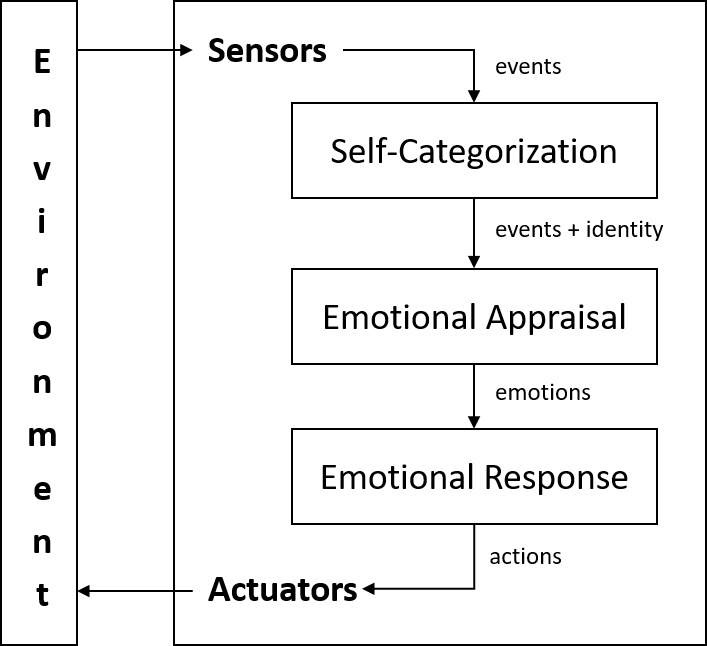
\includegraphics[width=0.3\textwidth]{images/gbe/model.png}
\caption{Diagram of the group-based emotions model.}
\label{fig:model}
\end{figure}


The first component of the model is the \textit{Self-Categorisation} component, which is responsible for managing the current context of the interaction as well as the social groups that are present in that context, if any, and their members. These elements constitute a social layer on top of the physical reality that is being perceived by the robot's sensors. Based on the Self-Categorisation Theory \cite{hornsey2008social,turner1987rediscovering}, when the robot detects a presence of an out-group then its own group identity will become more salient. 

The emotional appraisal is the second component of the model. This component is responsible for generating emotions in response to the events that occur within the current social context. An event can correspond to a performance of an action or to a change in a property of the environment. For each event perceived, the emotional component performs a series of value judgements about that event in relation to the robot. Then, a set of emotions are synthesised in accordance to those judgements. In emotional psychology, these judgements are referred to as appraisal variables with different theories of emotion proposing different sets of variables \cite{moors2013appraisal}. For instance, according to the OCC theory \cite{ortony1990cognitive}, when someone judges an event to be desirable for him or her, that person is likely to experience joy afterwards in proportion to the level of desirability attributed. The same theory also proposes that when someone performs an action that is considered blameworthy than that person is inclined to feel shame. However, if the blameworthy action is performed by another person, then a reproach emotion is felt instead by the observer.

While many researchers have already been able to integrate an emotional appraisal component in a social robotic architecture, the innovative aspect of our model lies in the notion that our appraisal component is capable of considering a social group as the actor of an event even if, in reality, all actions are being performed by individuals. This is the result of introducing the \textit{Self-Categorisation} component before the appraisal takes place in order to determine whether the robot sees itself and others acting based on their individual or their group identity. In the latter case, actions performed by individuals that are sharing the same group identity in the current context are appraised as if they are actions performed by the robot itself. Consequently, in a context where the robot is performing a team-based activity and one of its partners performs a blameworthy action, the appraisal component will generate in the robot a group-based emotion of shame, rather than a reproach emotion towards its partner.

Finally, the last component of the model is the \textit{Emotional Response} component, which is responsible for managing how the robot expresses the emotions that result from the appraisal process. This process must take into account the different possibilities that are afforded by the robot's embodiment. Assuming the robot has the ability to change its facial expression and body posture then these are matched to the current emotional state of the robot. In addition to non-verbal signals, the dialogue acts chosen by the robot are also influenced by its emotions. This is particularly important when trying to convey social emotions such as admiration or pride that can be hard to distinguish from more basic emotions as the ones proposed by Ekman \cite{ekman1987universals}, using only non-verbal modalities.

\begin{algorithm}[ht]
\caption{Group-based emotions generation process}
\label{algorithm-loop}
\begin{algorithmic}
\WHILE {\emph{true}}
\STATE$self \leftarrow Robot.Name $
\STATE$e \leftarrow Sensors.PerceiveNewEvent() $
\STATE$SG \leftarrow ContextManager.GetSalientSocialGroups() $ 
\IF{$SG \neq \emptyset $} 
\STATE$g \leftarrow IdentityManager.SelfCategorisation(SG, self)$ 
\IF{$e.ResponsibleAgent \in g$} 
\STATE $e.ResponsibleAgent \leftarrow g.Name$
\STATE $self \leftarrow g.Name$
\ENDIF
\ENDIF
\STATE$AV \leftarrow Appraisal.DetermineVariables(e)$
\STATE$E \leftarrow Appraisal.GenerateEmotions(AV, self)$
\STATE$se \leftarrow StrongestEmotion(E)$
\FORALL{$c \in Actuators.GetEmotionChannels()$}
\STATE$Express(se, c)$
\ENDFOR
\ENDWHILE
\end{algorithmic}
\end{algorithm}

Algorithm~\ref{algorithm-loop} provides a more detailed view of how these three components work together in a continuous cycle to create group-based emotions. As shown, the cycle starts by defining the parameter \textit{self} as equal to the robot's name, which should be a unique identifier of the robot. The next step is to check for the perception of a new event \textit{e} by the robot's sensors. Then, the set of salient social groups \textit{SG} is determined, taking into account the last event perceived. This set will be empty in the case where the current context or activity has no salient groups. If \textit{SG} is not an empty set then the group \textit{g} is selected as the one that the robot identifies the most with. Afterwards, the algorithm checks if the robot/person who caused the event to occur (\textit{e.ResponsibleAgent})  is a member of the same group \textit{g}. When that is the case, the event's responsible agent is replaced by the name of group \textit{g} as well as the parameter \textit{self}. At this point, the \textit{Self-Categorisation} component of the model ends and the \textit{Appraisal} component begins. Based on the event perceived \textit{e}, the set of appraisal variables \textit{AV} is now calculated. Subsequently, those variables are used to generate a set of emotions \textit{E}, from which the strongest emotion \textit{se} is extracted. The strongest emotion is considered to be the one with the highest intensity value. Finally, the emotion \textit{se} is expressed by all the available channels the robot has to express an emotion. 

Note that the algorithm presented here is aimed to be general enough so that it can be applied in different domains with different robots and using different models of appraisal and self-categorisation. As such, the use case that is described in the following section is to be viewed as just one possible way in which the proposed model can be fully implemented.

\section{Card game Scenario}
\label{sec:model-implementation}
In order to explore how group-based emotions influence human-robot teams, we used the described model to create social robots that are able to autonomously behave according to different levels of self-categorisation. We decided to choose a task with two adversarial teams to make the in-group and out-group distinction more prominent. The task chosen was \textit{Sueca}, a card game played by exactly four players divided in two opposing teams. Both cooperation with the partner and competition with the opponents have a strong effect on the game result since its goal is to beat the score of the other team. The players should play according to their understanding of their partners' game state. Another motivation for choosing a card game as our task comes from the fact that several studies \cite{ng2008memory,haring2014would,mccoll2013brian,shahid2014child} have demonstrated that card games are a successful activity for creating engagement in a human-robot interaction that is designed to be primarily social.


\textit{Sueca} is a trick-taking game containing the element of chance, and is played with a standard deck. The players start with ten cards in their hands, and have to decide which one to play during each trick. The suit of the first card played in a trick is considered to be the leadsuit of that trick and all players must follow it. If a player does not have any card from the leadsuit, then he or she is allowed to use a card with the trump suit, which is more valuable than the other suits. This is considered as ``cutting the trick''. The team that wins the trick consequently collects the sum of all its points. This occurs when any of its players played the highest trump card or the highest from the leadsuit when there is no trump card on the table.

With the aim of exploring mixed human-robot teams, our \textit{Sueca} scenario consists of two social robotic players that are both paired with a human partner. These robotic players are fully autonomous and their behaviours were developed on top of the SERA ecosystem \cite{ribeiro2016sera}. Players interact with the robots over a touch table using physical cards. The game application is then responsible for recognising the cards and forward all game events to the artificial players. Each of these artificial players is composed by an emotional agent \cite{dias2014fatima} and an AI \cite{correia2017asocial} that are responsible for the emotional behavioural responses and the game computations, respectively. Then, a behavioural planner schedules the non-verbal behaviours to the animation engine and the verbal behaviours to the Text-To-Speech (TTS).


\begin{table*}[ht]
\centering
\caption{Examples of speech acts performed by each robot according to the game state and the strongest appraised emotion.}
\label{tab:utterances-gbe}
\resizebox{\textwidth}{!}{%
\begin{tabular}{c|cccc|cccc}
                                                                          & \multicolumn{4}{c|}{Robot that expresses individual-based emotions}                                                                                                                                                                                                                             & \multicolumn{4}{c}{Robot that expresses group-based emotions}                                                                                                                           \\ \cline{2-9} 
                                                                          & Admiration                                                                 & Reproach                                                       & Pride                                                                 & Shame                                                                     & Admiration & Reproach & Pride                                                                            & Shame                                                                        \\ \hline
\begin{tabular}[c]{@{}c@{}}Partner\\ increased\\ trick score\end{tabular} & \begin{tabular}[c]{@{}c@{}}I am\\ impressed with\\ your move!\end{tabular} & ---                                                            & ---                                                                   & ---                                                                       & ---        & ---      & \begin{tabular}[c]{@{}c@{}}We are the\\ best!\end{tabular}                  & ---                                                                          \\ \cline{1-1}
\begin{tabular}[c]{@{}c@{}}Partner\\ decreased\\ trick score\end{tabular} & ---                                                                        & \begin{tabular}[c]{@{}c@{}}With that\\ move, I \\ cannot 
win. \end{tabular} & ---                                                                   & ---                                                                       & ---        & ---      & ---                                                                              & \begin{tabular}[c]{@{}c@{}}We were not\\ so good\\ this time...\end{tabular}    \\ \cline{1-9}
\begin{tabular}[c]{@{}c@{}}Robot\\ increased\\ trick score\end{tabular}   & ---                                                                        & ---                                                            & \begin{tabular}[c]{@{}c@{}}I played\\ incredibly\\ well!\end{tabular} & ---                                                                       & ---        & ---      & \begin{tabular}[c]{@{}c@{}}I am impressed\\ with our\\ performance!\end{tabular} & ---                                                                          \\ \cline{1-1}
\begin{tabular}[c]{@{}c@{}}Robot\\ decreased\\ trick score\end{tabular}   & ---                                                                        & ---                                                            & ---                                                                   & \begin{tabular}[c]{@{}c@{}}I am so\\ ashamed of\\ my move...\end{tabular} & ---        & ---      & ---                                                                              & \begin{tabular}[c]{@{}c@{}}Sorry partner,\\ for this\\ unfortunate move.\end{tabular}
\end{tabular}}
\end{table*}


Although the two robots have the same embodiment and the same interaction affordances, one of them generates group-based emotions and the other generates individual-based emotions. This is accomplished in the following manner. Following Algorithm~\ref{algorithm-loop}, each robot starts by identifying itself with its name, among the four possible players ($\{P1,...,P4\}$).
The robot then perceives game events associated to the plays made by players and corresponding changes in the game state such as ``$Event(P3,IncreasePoints(Trick, 11))$''. In the context of \textit{Sueca} there are two salient social groups, which correspond to the two teams playing ($SG = \{T1, T2\}$). 



The following step of \textit{SelfCategorisation} differentiates our two robots. Although this process in humans can be highly complex, our implementation for this particular scenario follows a rather simple logic. Namely, for the robot that expresses group-based emotions this step returns the team to which the robot belongs. For the example above, assuming that the robot is $P1$ and also that $P1 \in T1$, $T1$ will be assigned to $g$. Then, verifying the responsible agent ($P3$) belongs to that same social group, $T1$ will be assigned to both $e.ResponsibleAgent$ and $self$. In other words, the robot attributes the responsibility of the perceived event to its social group, instead of its partner, and appraises the event on behalf of the group.

On the contrary, the robot that expresses individual-based emotions was implemented without the self-categorisation step, which will lead it not to identify itself as a member of a social group, regardless of the groups contained in $SG$. In other words, the robot without self-categorisation attributes the responsibility of the perceived event always to an individual, instead of a social group, and consequently appraises events as an individual.

The appraisal and emotional generation steps of the proposed model were implemented with FAtiMA \cite{dias2014fatima}, an existing emotional architecture that is based on the OCC theory \cite{ortony1990cognitive}. In our scenario, two appraisal variables of the OCC theory were used, namely, \textit{Desirability} and \textit{Praiseworthiness}. Using the rule-based mechanism present in FAtiMA, the value of these two variables are determined in the following manner. All the plays made by an opponent that increase/decrease the points of the trick for the robot's team are considered to be desirable/undesirable by an amount that is linearly proportional to the number of points increased/decreased. In the case of the plays made by the robot or its partner, if they increase/decrease the points of the trick they are seen as praiseworthy/blameworthy, also in a linearly proportional manner. 

Once the appraisal variables are determined, the step of generating emotions occurs. Based on the OCC model, a positive/negative value of desirability generates an emotion of joy/distress. As for praiseworthiness, if it is positive, an emotion of pride or admiration is generated based on the event's responsible agent. Pride in the case where it matches the robot's \textit{self} parameter and admiration otherwise. Inversely, if praiseworthiness is negative then an emotion of shame or reproach is generated instead. Shame in the case where it matches the robot's \textit{self} parameter and reproach otherwise. Finally, the emotional response of our robots is based on the current strongest emotion. The responses may be utterances of verbal and non-verbal behaviour or physical postures.




\subsection{Emotional Response}
The behaviours and emotional responses of each robot may differ according to the properties of its embodiment. In our scenario, the EMYS robot \cite{kkedzierski2013emys} was used and its behaviours include utterances (i.e., dialogue acts, gazes, and animations) and physical postures. 

\subsubsection{Utterances}
In total, two sets of utterances were created to convey the emotional state of the robots. One set was used by the robot with individual-based emotions and the other was employed by the robot with group-based emotions. In order for their dialogue acts to convey the nature of the emotion generated by the model, they may contain inclusive pronouns (e.g., ``we'', ``us'', ``our'') to express group-based emotions, or individual pronouns (e.g., ``I'', ``me'', ``you'') to suggest individual-based emotions. This distinction becomes more relevant to unambiguously distinguish emotions such as ``Individual Pride'' and ``Group Pride''. A similar language adaptation was employed by Brave et al. \cite{brave2005computers} to differentiate between self- vs. other oriented emotions.

The full list of utterances is available in \cite{correia2018} and contains about 100 utterances for each robot. Each robot has an extensive repertoire of sentences in order for the robots not to repeat themselves during the interaction, which lasts approximately 30 minutes with both robots interacting fully autonomously. Moreover, we tried to differentiate the wording of the sentences for both robots (while maintaining the same meaning), instead of solely changing the pronouns. Otherwise, it would seem that the robots were repeating each other and this could significantly break their believability as two independent social actors. 

The selection of utterances takes into account the current game state and their strongest emotion. To be more precise, there are four particular game states where the robots have different emotions and, therefore, result in different behaviours, as evidenced by Table~\ref{tab:utterances-gbe}. 

Note that in the case where an opponent is playing, the robotic characters will only interact verbally in emotionally neutral situations (e.g. greeting, ask to shuffle). In emotionally charged situations, such as when an opponent cuts the trick, the robots will only express an emotion of joy or distress through non-verbal animations. Therefore, independently of the self-categorisation level of the robots, they react similarly towards the out-group.



We have validated all the utterances by asking three coders to classify the associated strongest emotion, among the possible 6 of joy, distress, pride, admiration, shame, or reproach. The average pairwise Cohen's kappa value was k=0.82, revealing good agreement between the coders and that the chosen sentences accurately reflect their intended emotions.

\subsubsection{Postures}

Another non-verbal behaviour of the robotic characters was the embodiment posture. While utterances and simple animations convey a reaction upon a particular game event, a posture is used to convey for a longer period of time the emotional state of the robots. During the turn of other players, the robots choose the strongest emotion to adapt their postures, see Figure~\ref{fig:postures}.

\begin{figure}[ht]
    \centering
    \begin{subfigure}{0.2\columnwidth}
        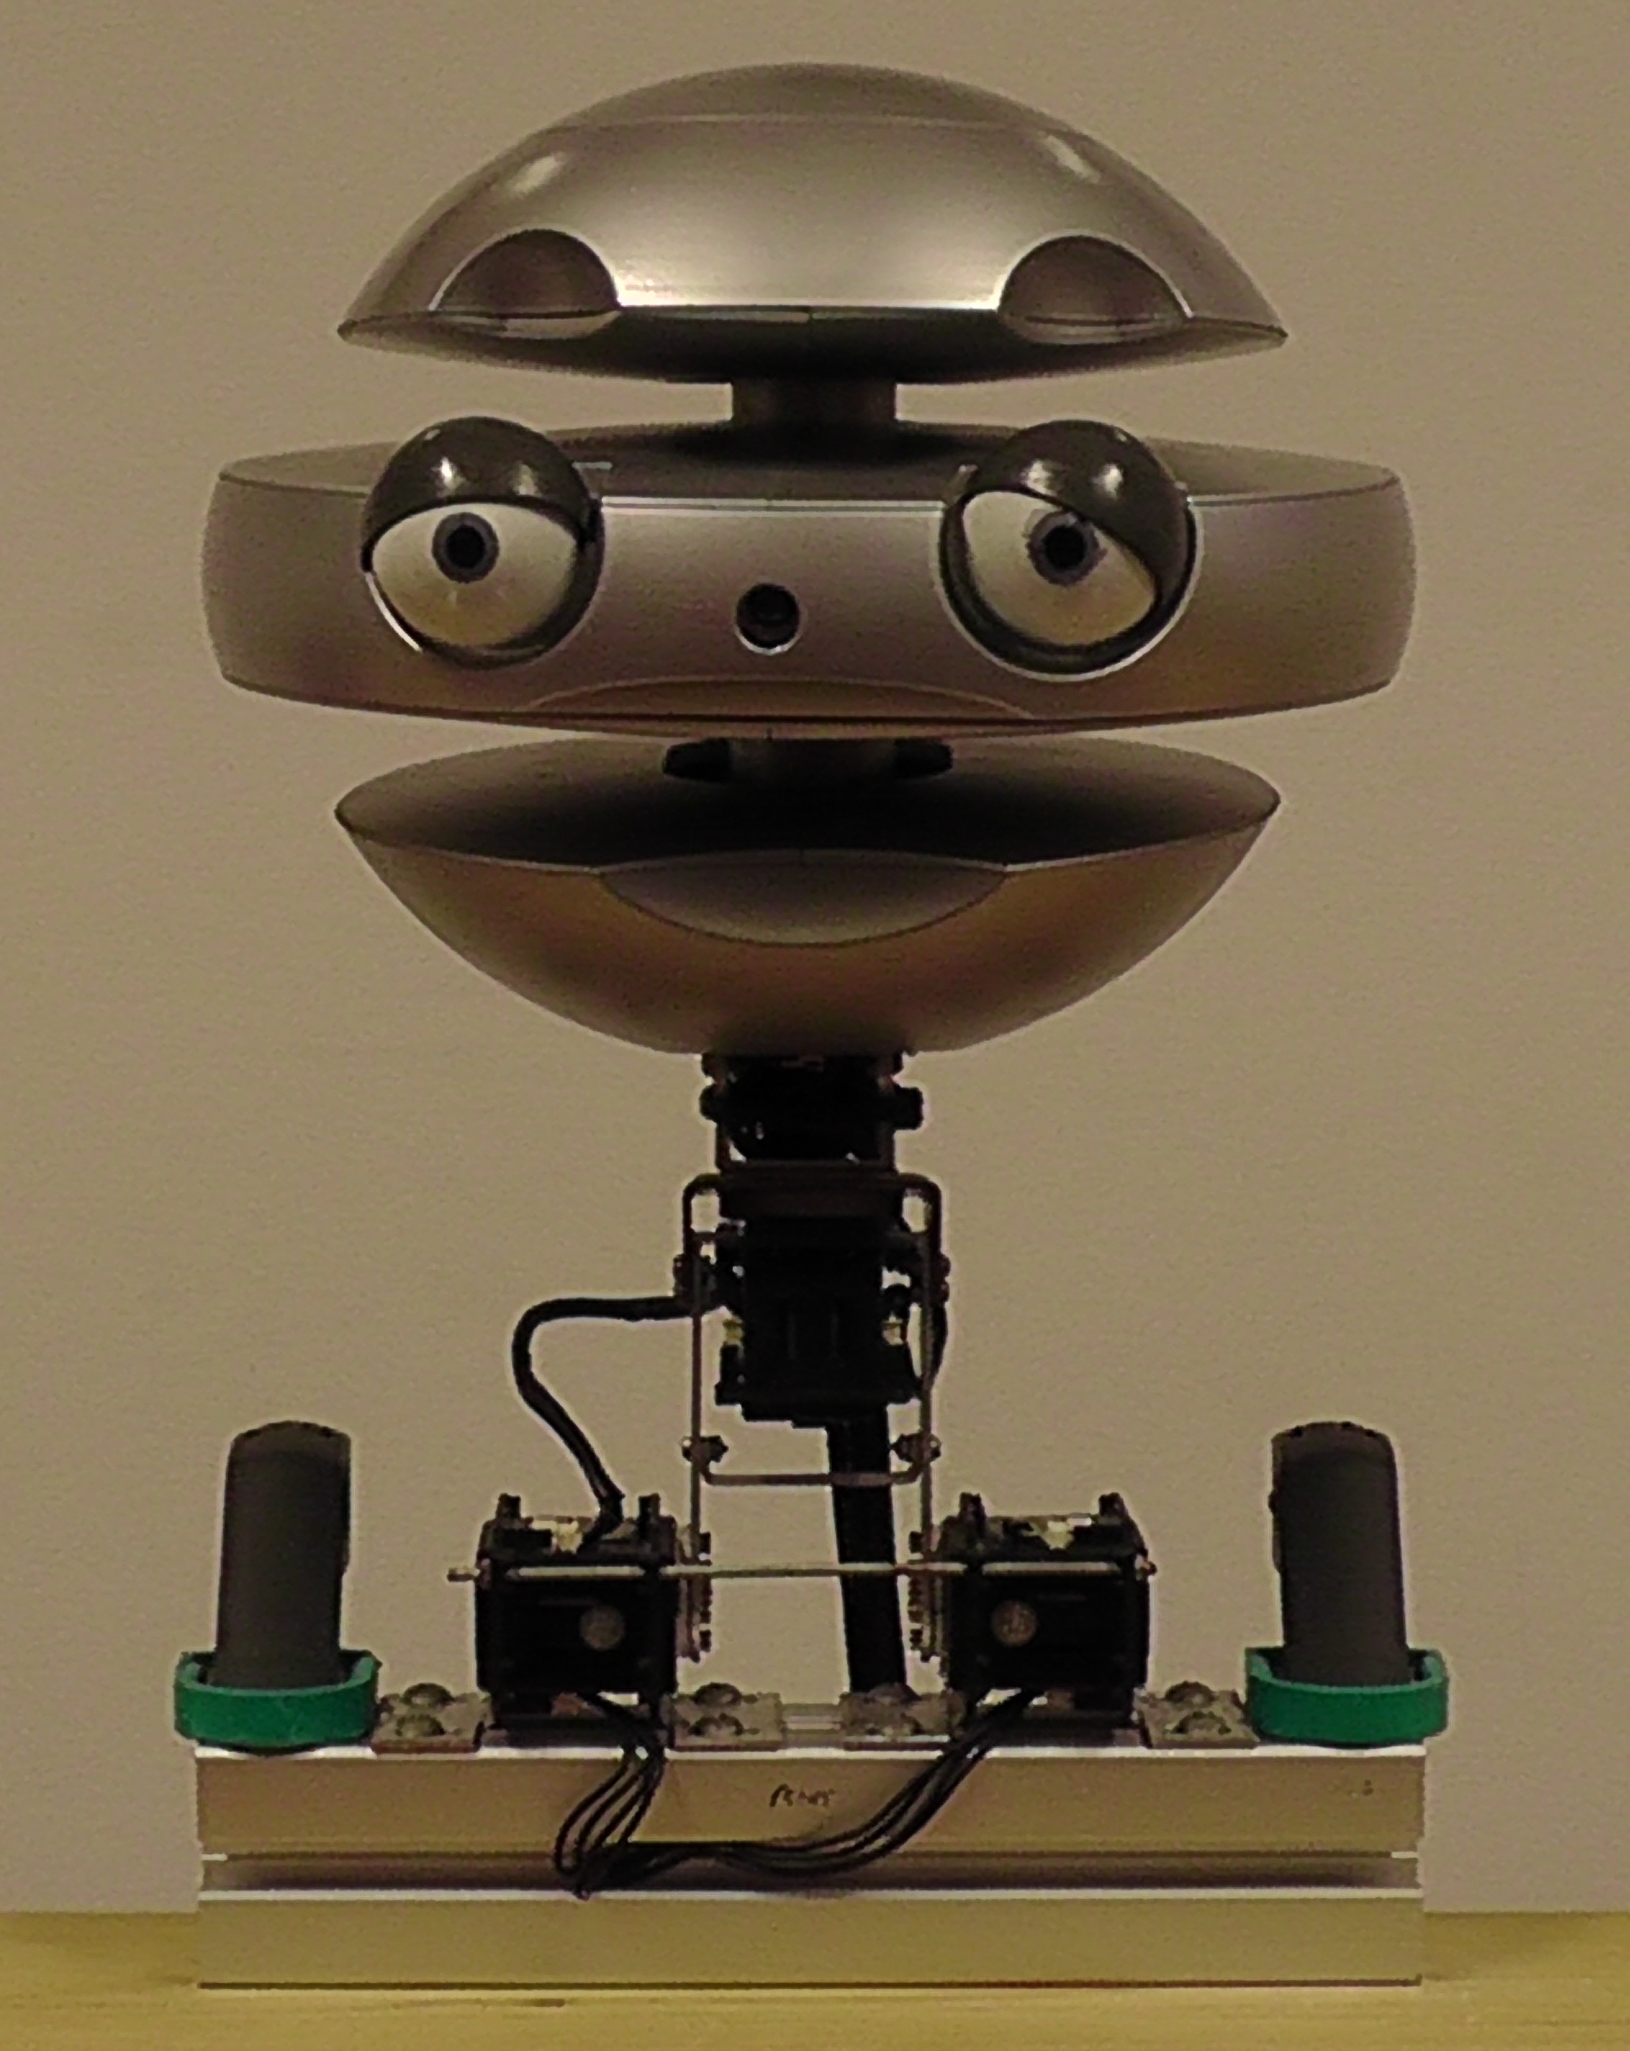
\includegraphics[width=\columnwidth]{images/gbe/joy.jpg}
        \caption{Joy}
    \end{subfigure}
    \begin{subfigure}{0.2\columnwidth}
        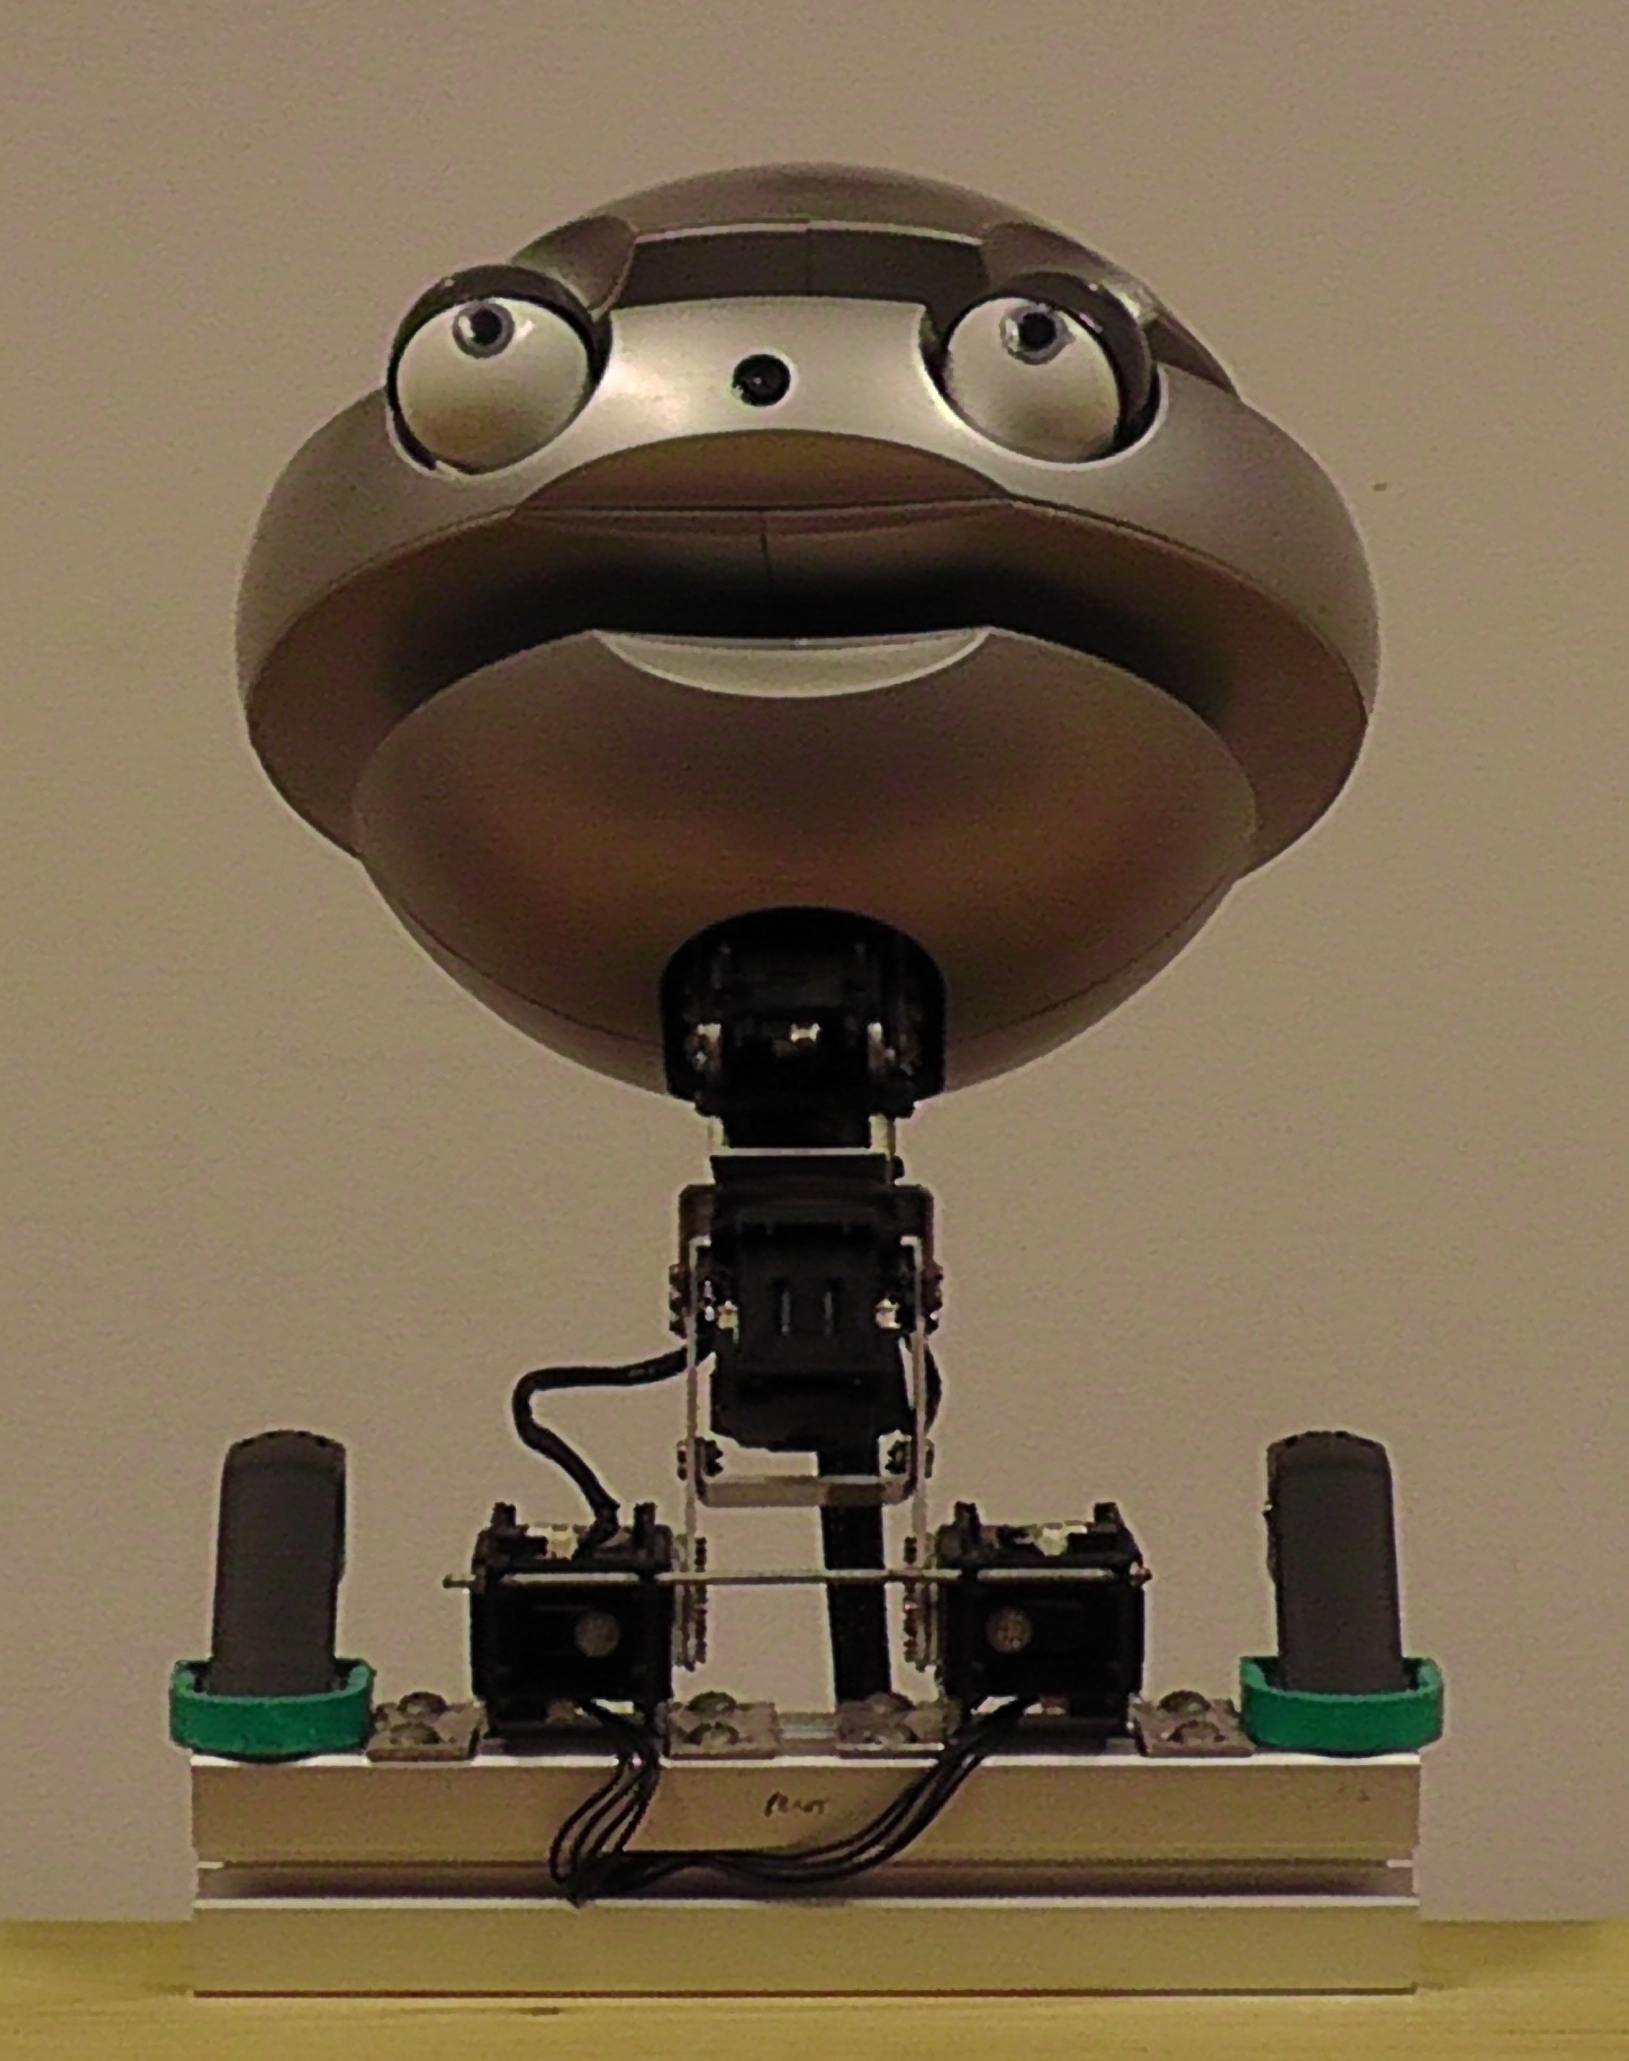
\includegraphics[width=\columnwidth]{images/gbe/pride.jpg}
        \caption{Pride}
    \end{subfigure}
    \begin{subfigure}{0.2\columnwidth}
        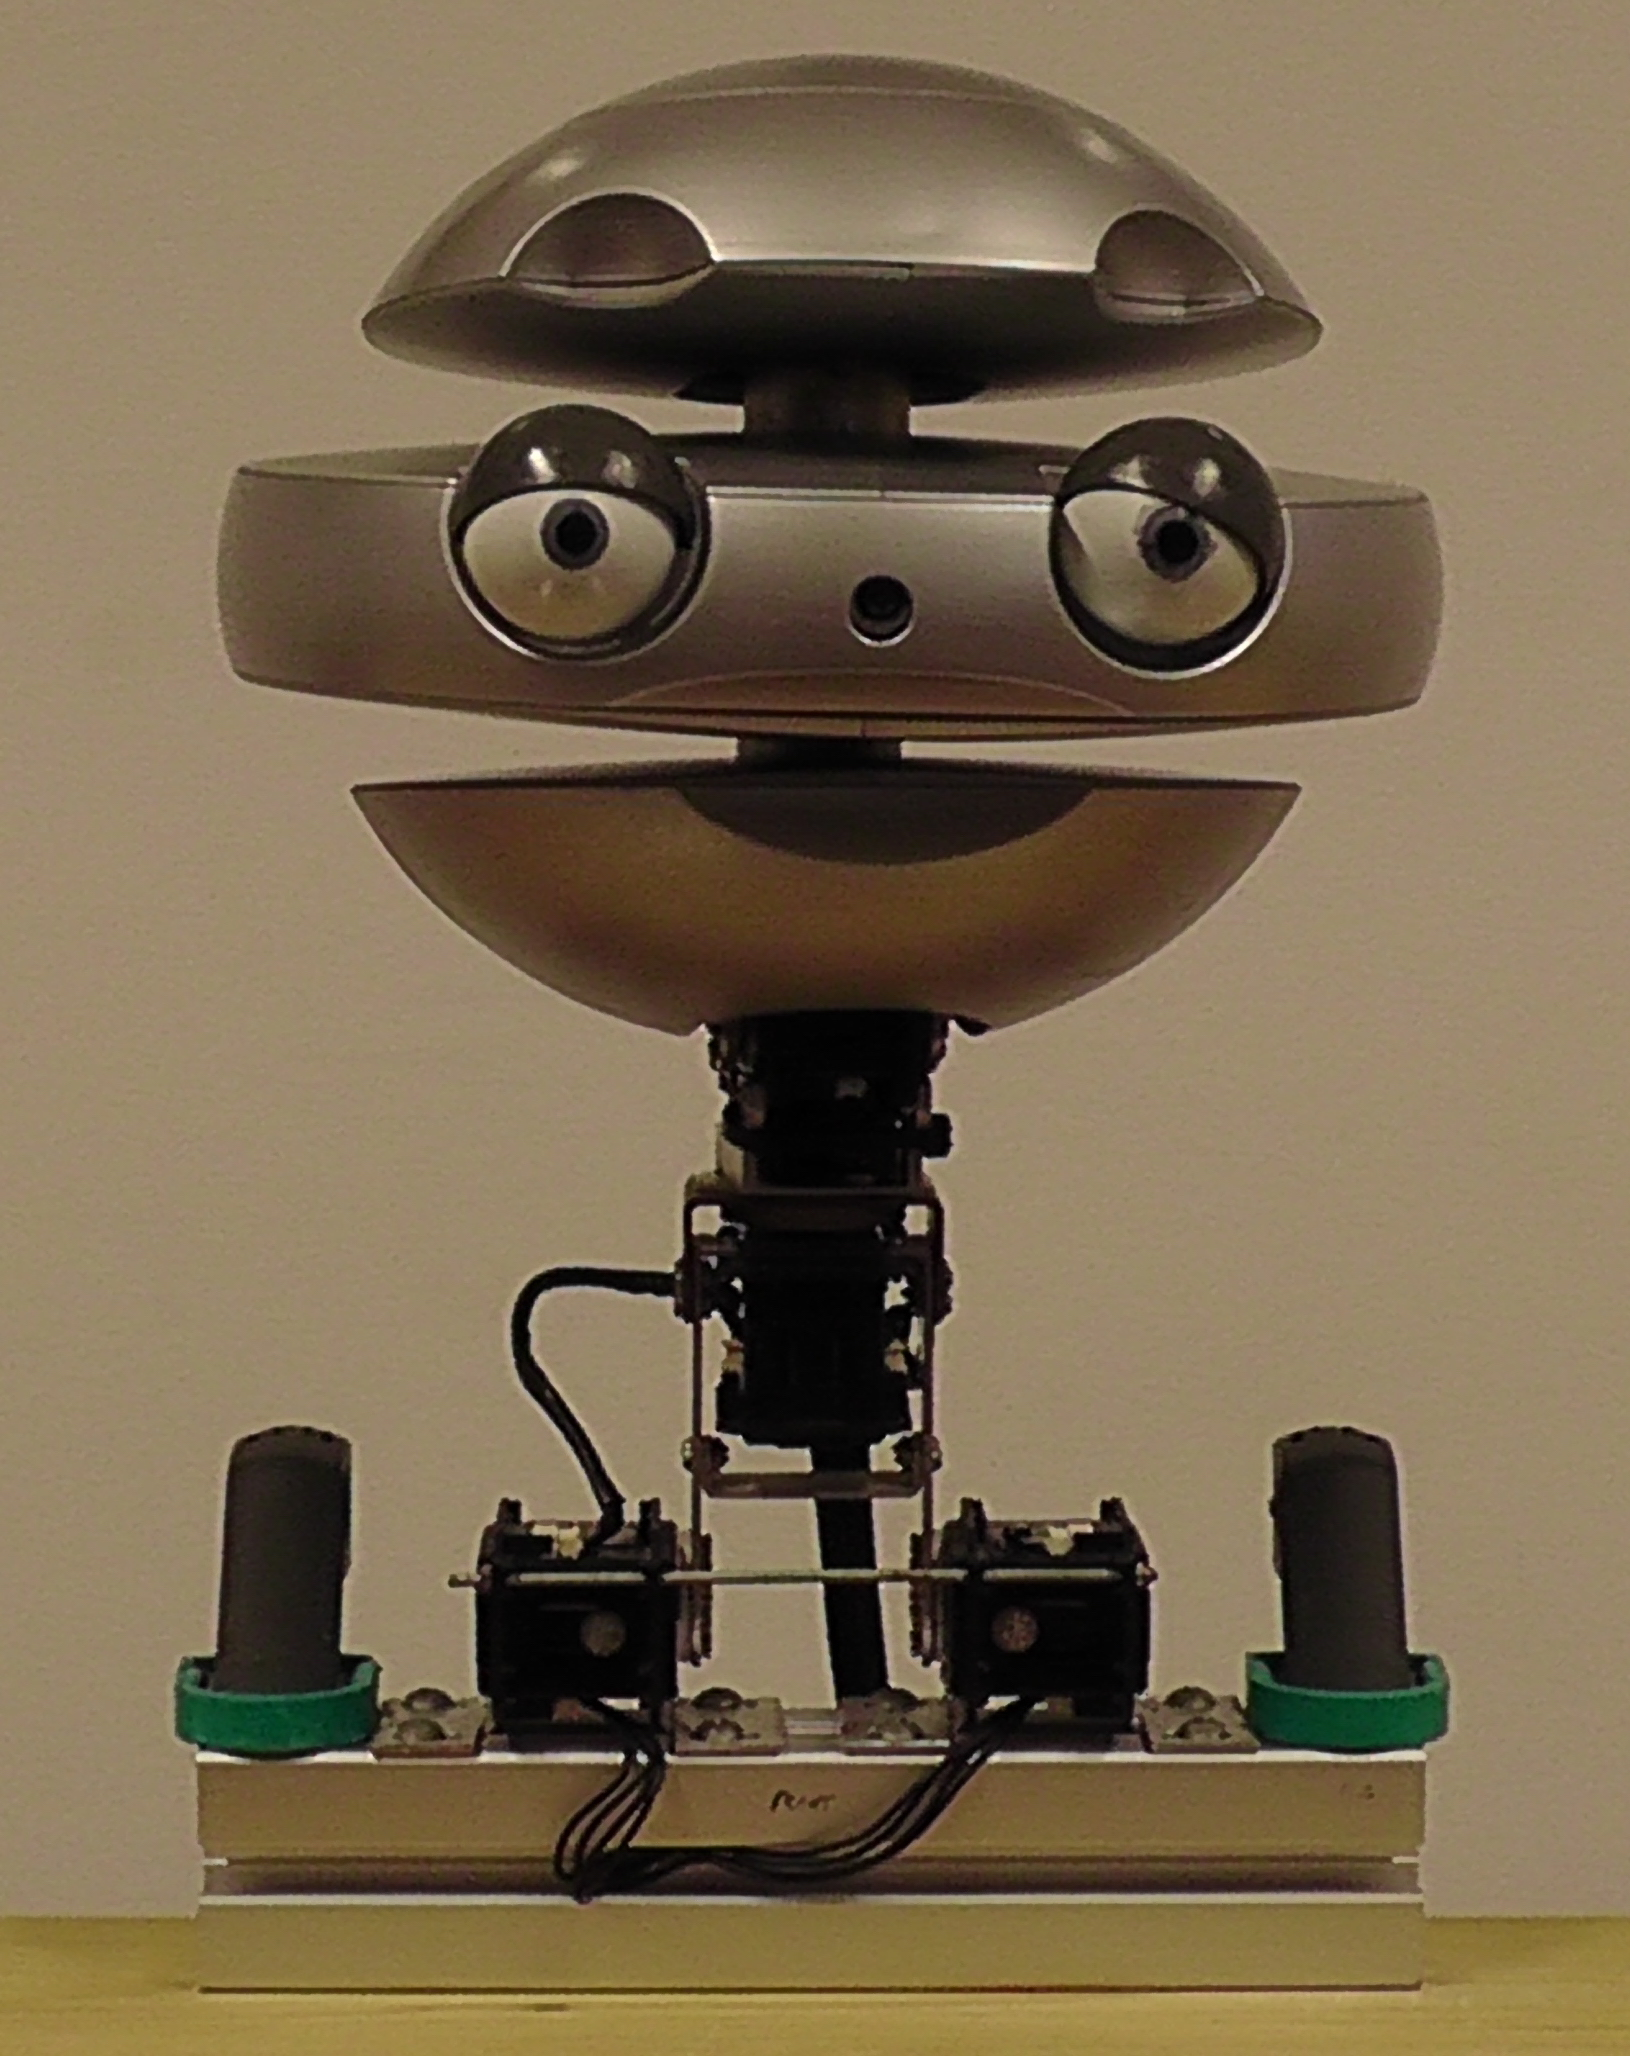
\includegraphics[width=\columnwidth]{images/gbe/admiration.jpg}
        \caption{Admiration}
    \end{subfigure}
    
    \begin{subfigure}{0.2\columnwidth}
        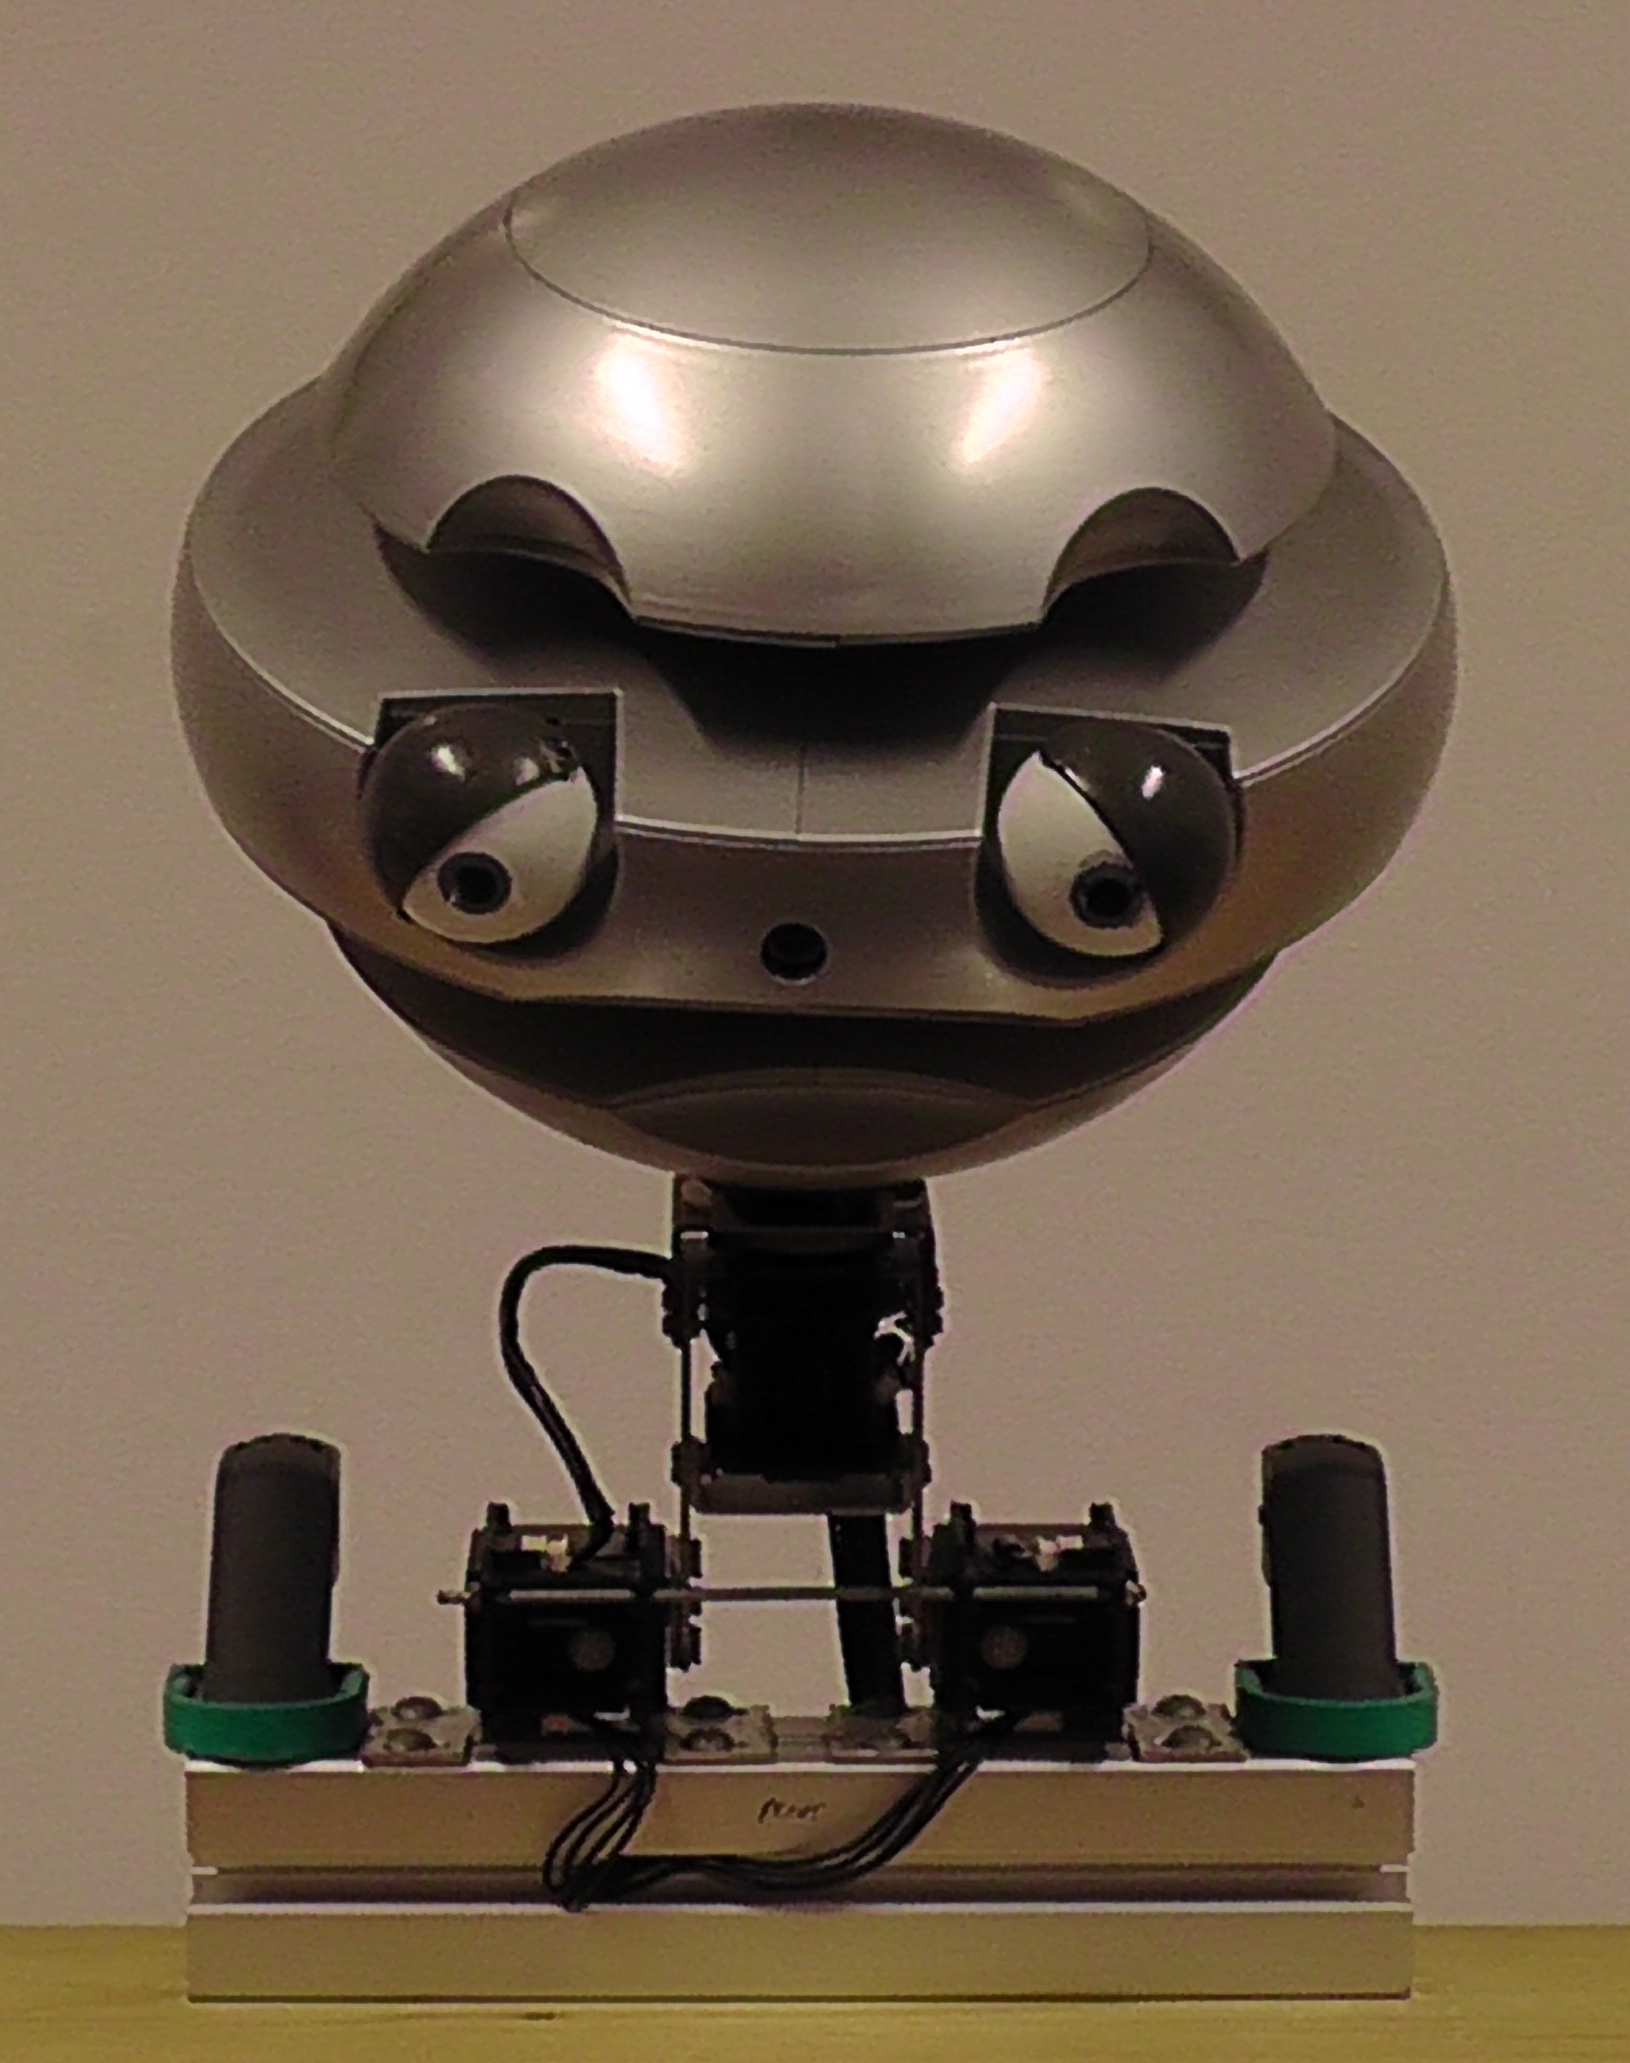
\includegraphics[width=\columnwidth]{images/gbe/distress.jpg}
        \caption{Distress}
    \end{subfigure}
    \begin{subfigure}{0.2\columnwidth}
        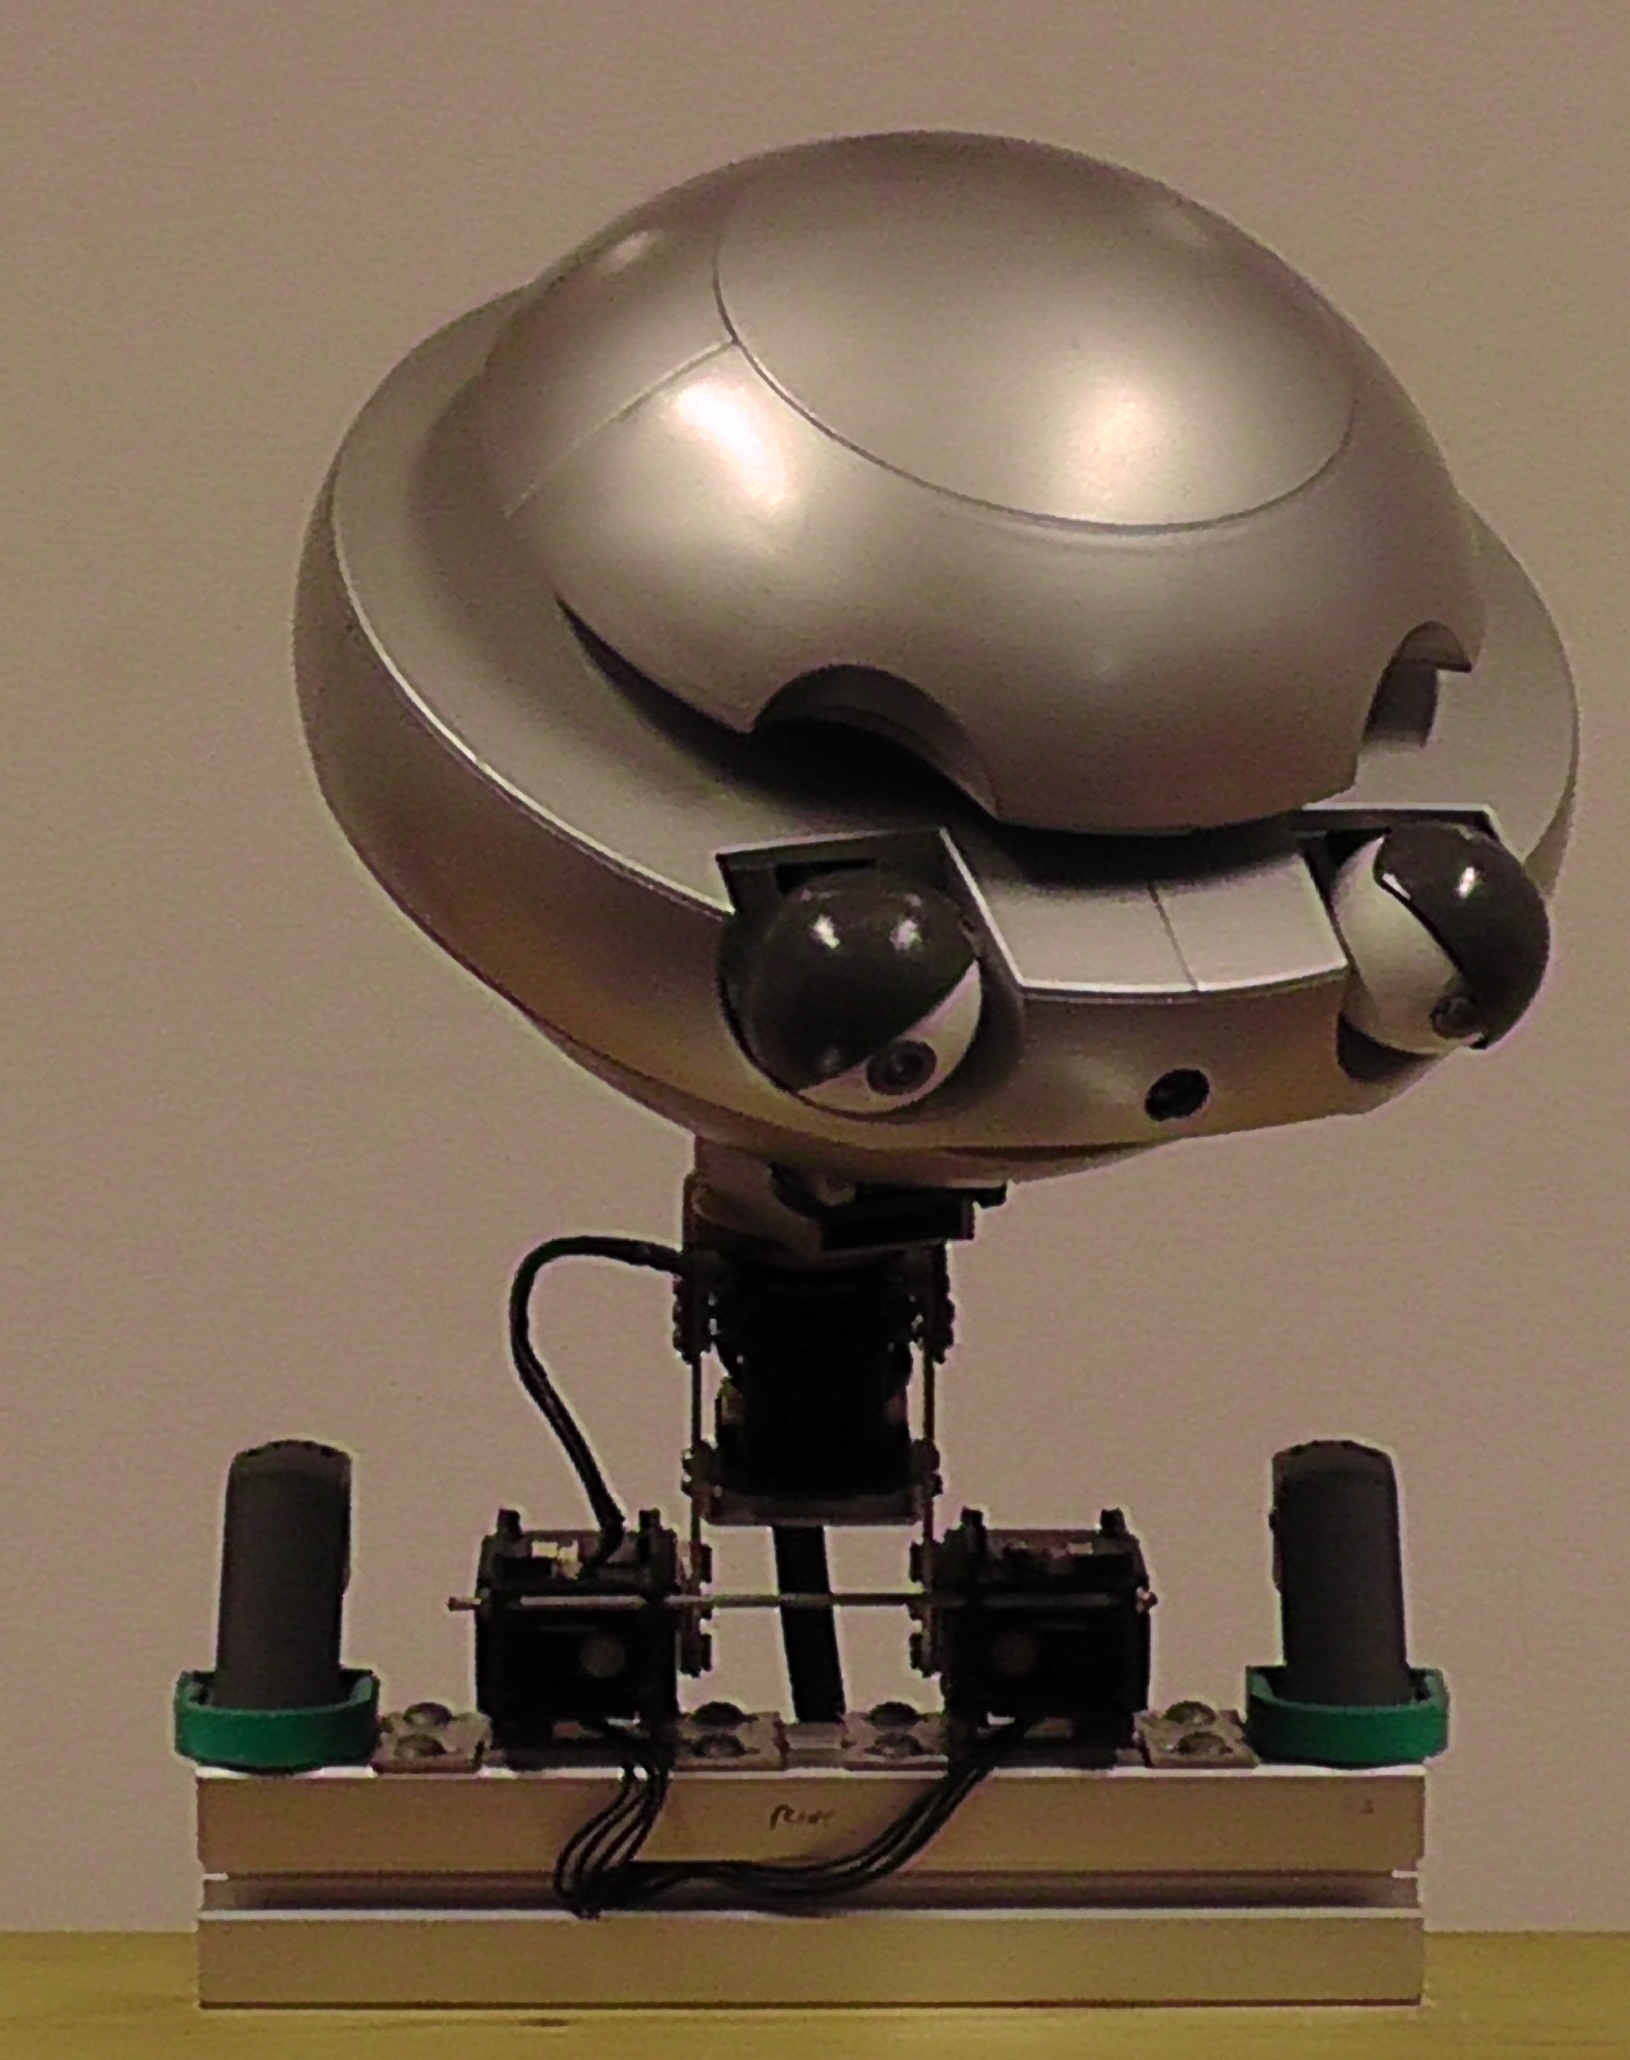
\includegraphics[width=\columnwidth]{images/gbe/shame.jpg}
        \caption{Shame}
    \end{subfigure}
    \begin{subfigure}{0.2\columnwidth}
        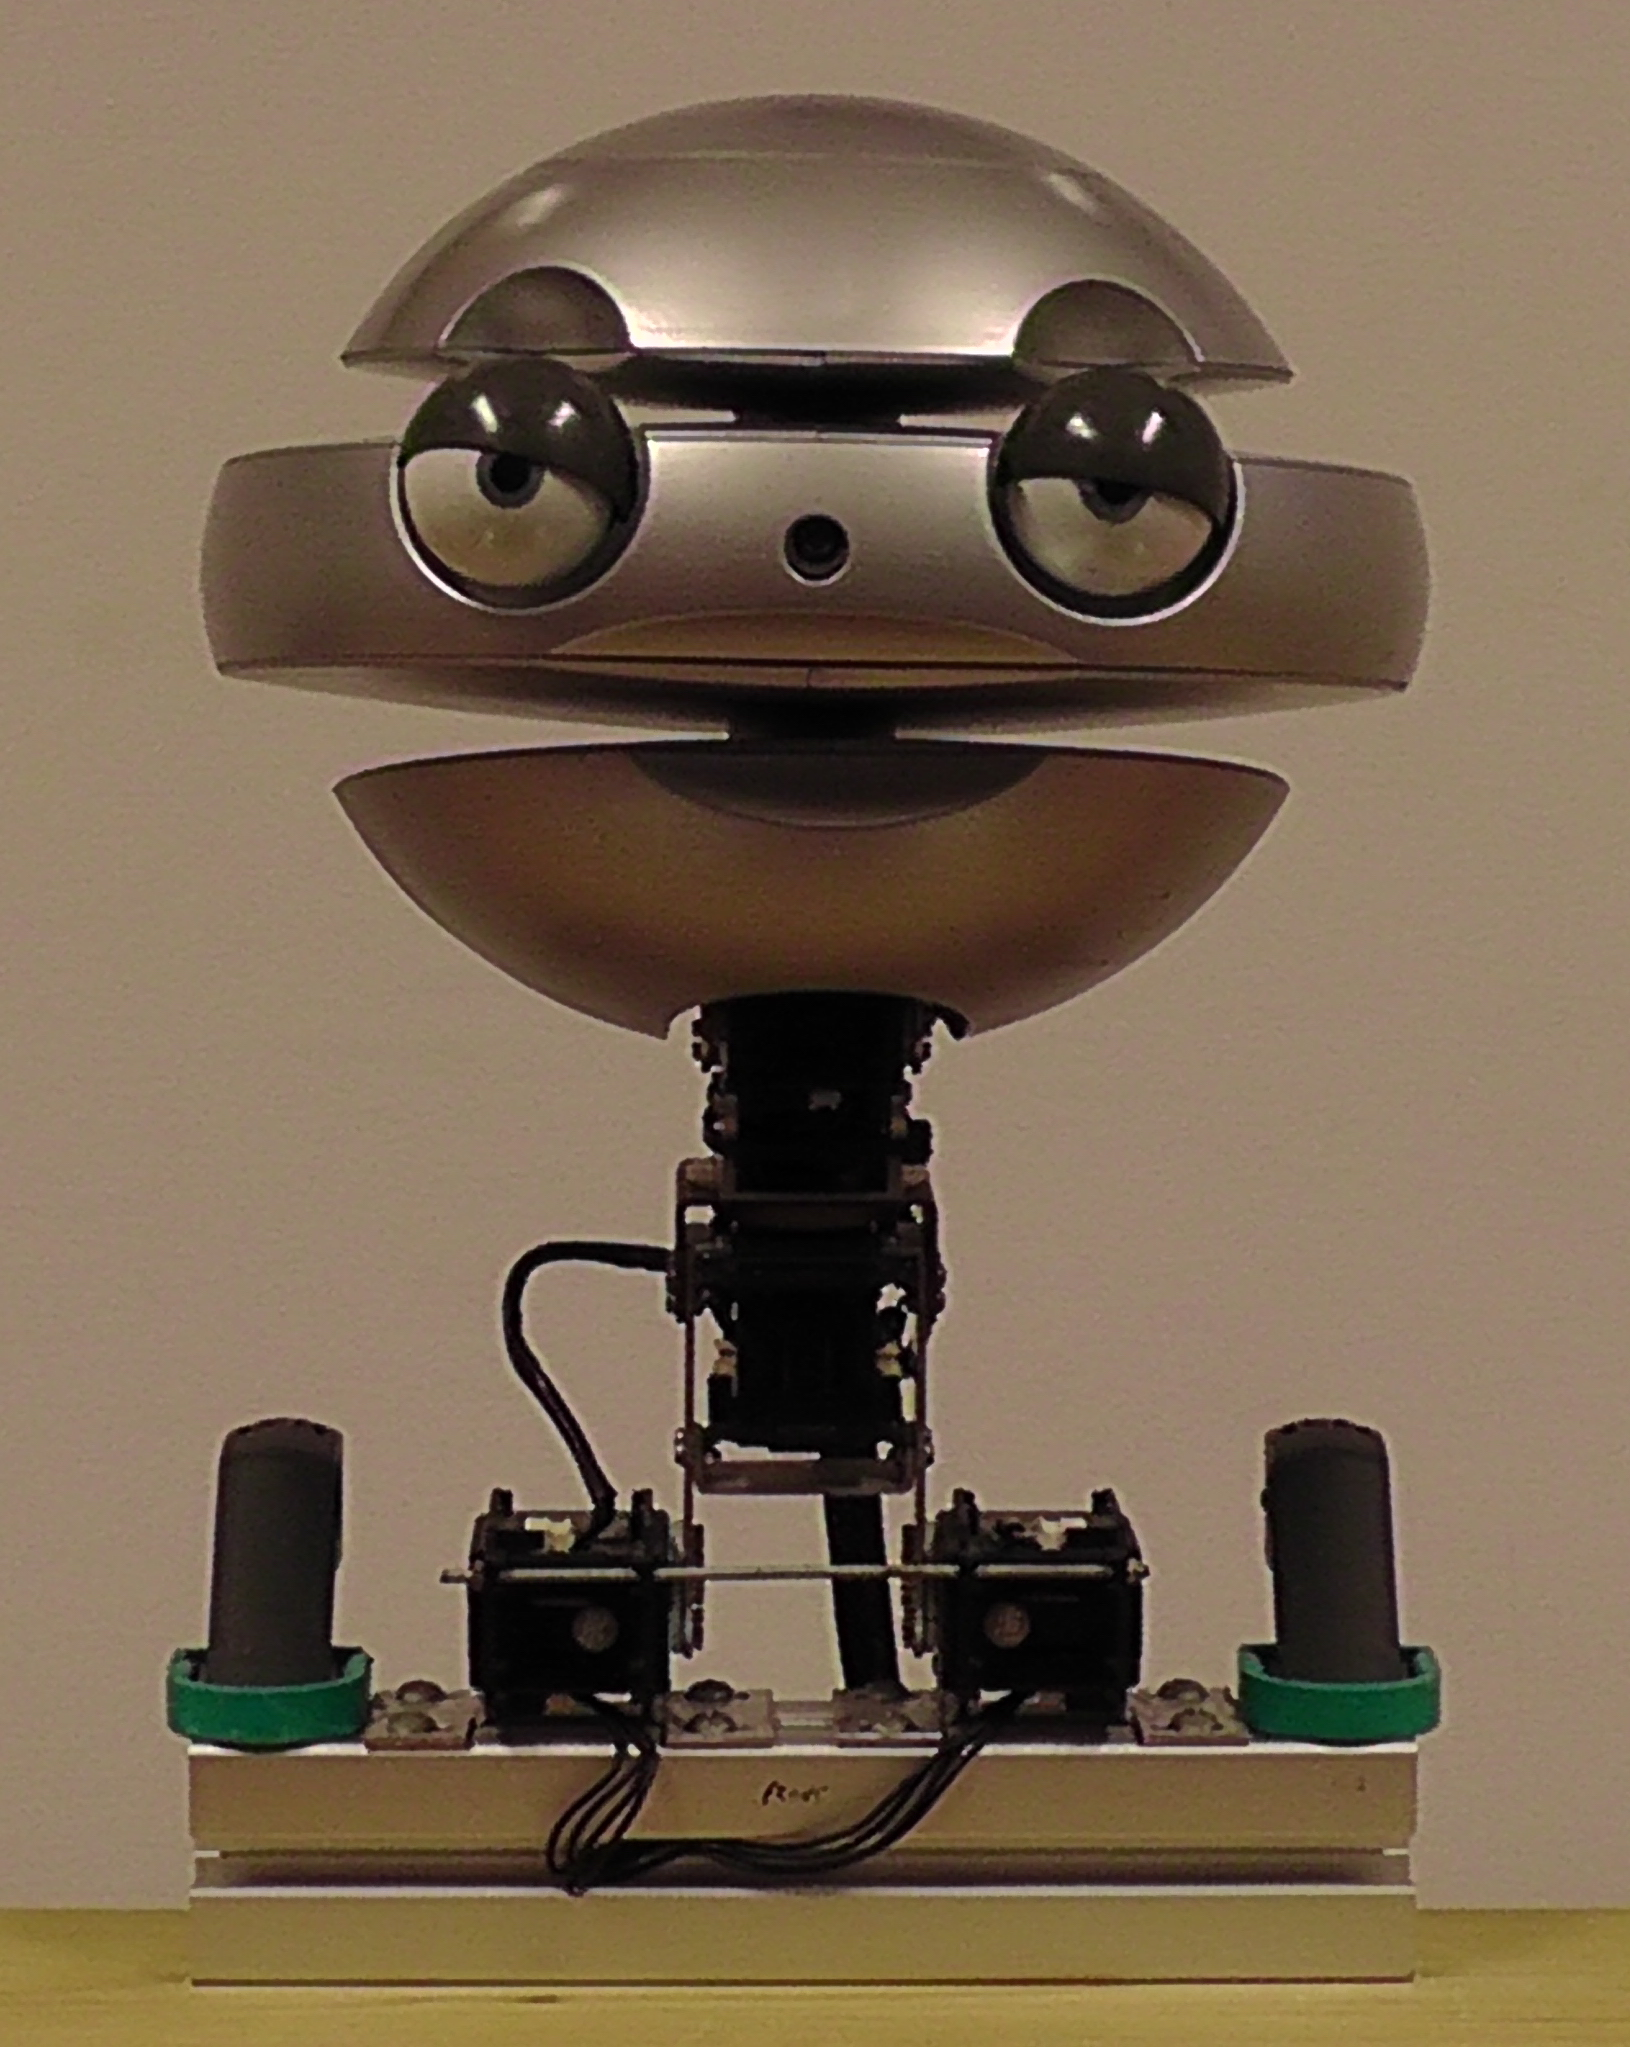
\includegraphics[width=\columnwidth]{images/gbe/reproach.jpg}
        \caption{Reproach}
    \end{subfigure}
    \caption{Postures embodied on the EMYS robot for each emotion.}
    \label{fig:postures}
\end{figure}


\section{User study}
\label{sec:study4}
Using the Sueca scenario described in the previous section, we conducted a user study where two participants form a team with a robot to play the card game. We used the same embodiment -- EMYS robot -- although the robots expressed different types of emotions: group-based or individual-based emotions. Based on the previously discussed findings from intergroup interactions in human-human \cite{kessler2005group,allen2004exploring} as well as in human-robot \cite{kuchenbrandt2013robot,haring2014would,desai2012effects,wang2016trust} scenarios, we expect to check the following hypothesis:

\textbf{H1:} Participants will have a stronger Group Identification with a robotic partner that expresses group-based emotions.

\textbf{H2:} Participants will have a more positive perception of a robotic partner that expresses group-based emotions.

\textbf{H3:} Participants will have a higher degree of Group Trust with a robotic partner that has group-based emotions.


\subsection{Procedure}
Each session of the experiment had two participants and took approximately 45 minutes. Participants read a consent form and were briefly introduced to the game activity. The game rules were described and two researchers played a sample game with the participants over a regular wooden table. Then, participants were randomly assigned to one robotic partner -- which could express either group-based or individual-based emotions--, and moved to the touch table, where they played three consecutive games with the robots, see Figure~\ref{fig:user-study}.
In the beginning one researcher explained how the game works over the touch table and the initial setup of assigning the robots' cards. At the same time, another researcher would set two cameras for video recording if participants had authorised. A researcher stayed in the experiment room until the end of the first trick. After this, both researchers left the room and let participants play the three games. Finally, they were given a questionnaire and the experiment ended with a cinema ticket being randomly awarded to one of the participants.

\begin{figure}[ht]
    \centering
    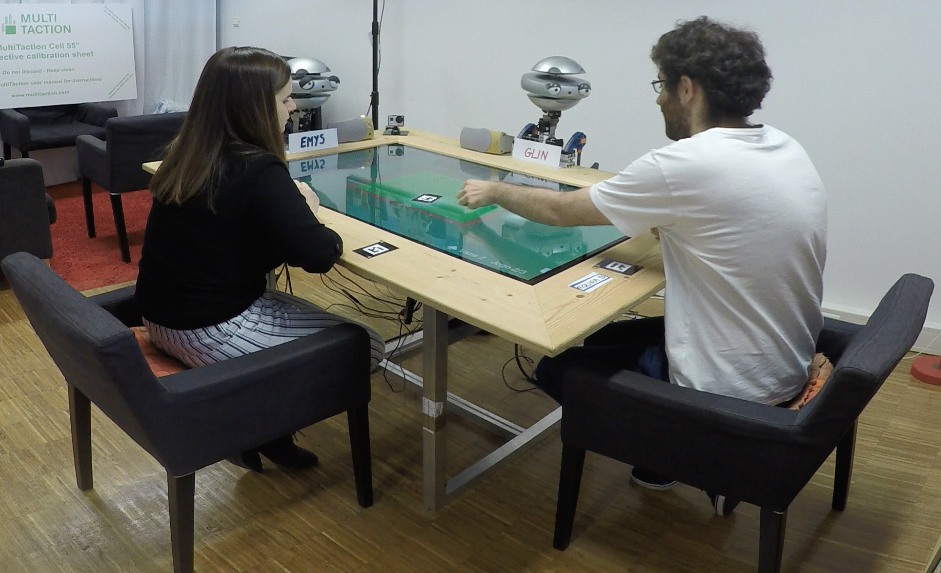
\includegraphics[width=0.7\columnwidth]{images/gbe/interaction}
    \caption{Experimental setting for the user study.}
    \label{fig:user-study}
\end{figure}



\subsection{Measures}
Independently of the robotic partner, all participants answered a  final questionnaire that contained the following measures:
\begin{itemize}
\item \textbf{Group Identification} \cite{leach2008group}
with the Portuguese adaptation \cite{ramos2011adaptaccao} 
to assess the in-Group Identification with their robotic partner;
\item \textbf{Godspeed Questionnaire} \cite{bartneck2009measurement}, using the dimensions of Anthropomorphism, Animacy, Likeability, and Perceived Intelligence regarding their robotic partner;
\item \textbf{Group Trust} \cite{allen2004exploring} to assess the perceived trust by the participants regarding their team in the game;
\item \textbf{Demographic questions}, i.e. gender, age, previous interaction with the EMYS robot, proficiency level in the \textit{Sueca} card game.
\end{itemize}
Both Group Identification and Group Trust measures used 7-points Likert Scales, ranging from Strongly Disagree to Strongly Agree. The Godspeed Questionnaire was assessed in 5-points semantic differential scale.

\subsection{Sample}
We recruited a total of 48 university students (33 males and 15 females) with ages ranging from 19 to 33 years old ($M=25.02\pm 2.98$). 25\% of the participants had already interacted with the EMYS robot and 77.1\% reported at least a medium proficiency level of playing the \textit{Sueca} card game.

\subsection{Results}
In the 24 collected sessions, the team of the robot with group-based emotions won 10 times, lost 11 times, and tied 3 times. Table~\ref{tab:utterances-couning} shows the number of utterances performed by each robot for each emotion and evidences a balanced average of total utterances per session. As expected, in both conditions there were more utterances for positive emotions in general than for negative ones. This can be attributed to the fact that players naturally avoided making bad plays as they were trying to win. Given that some of the following measures did not show normal distributions (as indicated by the Shapiro-Wilk test), we used the non-parametric Mann-Whitney U-test to compare the independent samples.

\begin{table}[ht]
\centering
\caption{Average number of utterances per emotion for the Robot with Group-based Emotions (RGbE) and the Robot with Individual-based Emotions (RIbE).}
\label{tab:utterances-couning}
\begin{tabular}{c|ccccccc|c}
     & Neutral & Admiration & Reproach & Pride & Shame & Joy & Distress & \textbf{TOTAL} \\ \hline
RGbE & 6       & 0          & 0        & 15    & 4     & 4   & 5        & 34             \\
RIbE & 6       & 7          & 2        & 6     & 2     & 4   & 8        & 35            
\end{tabular}
\end{table}



\subsubsection{Group Identification}
A reliability analysis was carried out on the satisfaction and solidarity dimensions comprising 4 and 3 items, respectively. Cronbach's alpha of 0.83 for the satisfaction dimension, and 0.81 for the solidarity dimension indicate a high level of internal consistency for the scale of Group Identification with this specific sample.

We compared the level of Group Identification perceived by the participants towards each robot. Participants had significantly higher levels ($U=175.5, p=0.02, r=0.335$) of Group Identification towards the robotic partner with group-based emotions ($M=5.94\pm0.17$) than towards the robotic partner with individual-based emotions ($M=5.22\pm0.22$), see Figure~\ref{fig:group-measures}.

Additionally, a Spearman's rank-order correlation was run to determine if there was a relationship between the number of points of the team and the Group Identification metric. The rationale was to check if having more points as a consequence of winning the game would also have a positive effect on this dimension. The correlation was non-significant ($r_s=0.153$, $p=0.30$), which suggests that these two factors are independent. 



\begin{figure}[ht]
    \centering
    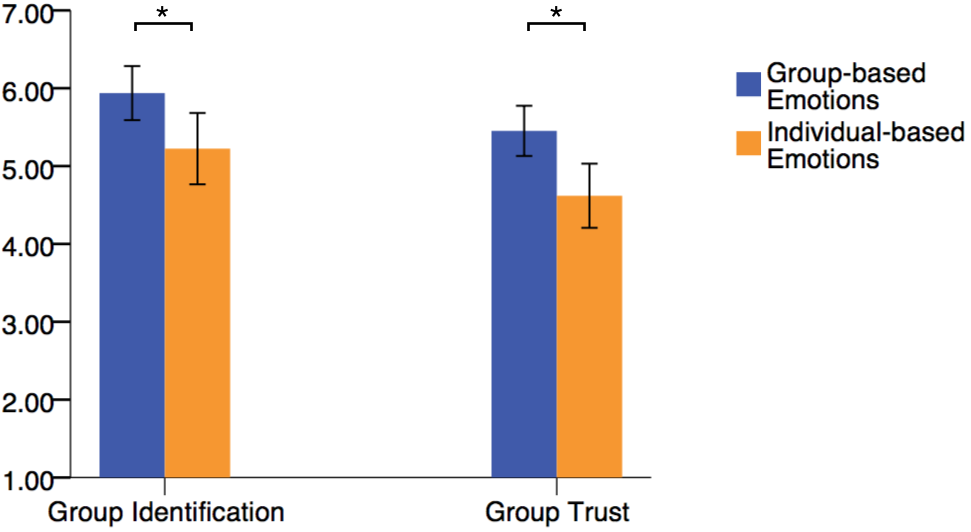
\includegraphics[width=0.6\columnwidth]{images/gbe/group2.png}
    \caption{Group Identification and Group Trust averages attributed to each team with a robot that expresses either group-based or individual-based emotions. (*$p<0.05$)}
    \label{fig:group-measures}
\end{figure}

\subsubsection{Perception of the robots}

To check whether the expression of individual or group-based emotions was influencing the perception of the robots, we compared the levels of Anthropomorphism, Animacy, Likeability and Perceived Intelligence attributed to each robot. Results showed no significant differences in the Anthropomorphism ($U=276, p=0.80$), Animacy ($U=275, p=0.79$), and Perceived Intelligence ($U=200, p=0.07$) levels attributed to robotic partner with group-based emotions ($M_{ant}=2.97\pm0.14;M_{ani}=3.57\pm0.13;M_{pi}=3.91\pm0.14$) and the robotic partner with individual-based emotions ($M_{ant}=2.95\pm0.17;M_{ani}=3.50\pm0.14;M_{pi}=3.47\pm0.17$), see Figure~\ref{fig:godspeed}. However, participants attributed significantly higher scores of Likeability ($U=142.0, p=0.002, r=0.437$) to the robotic partner with group-based emotions ($M=4.33\pm0.11$) than the robotic partner with individual-based emotions ($M=3.49\pm0.21$), see Figure~\ref{fig:godspeed}.


\begin{figure}[ht]
    \centering
    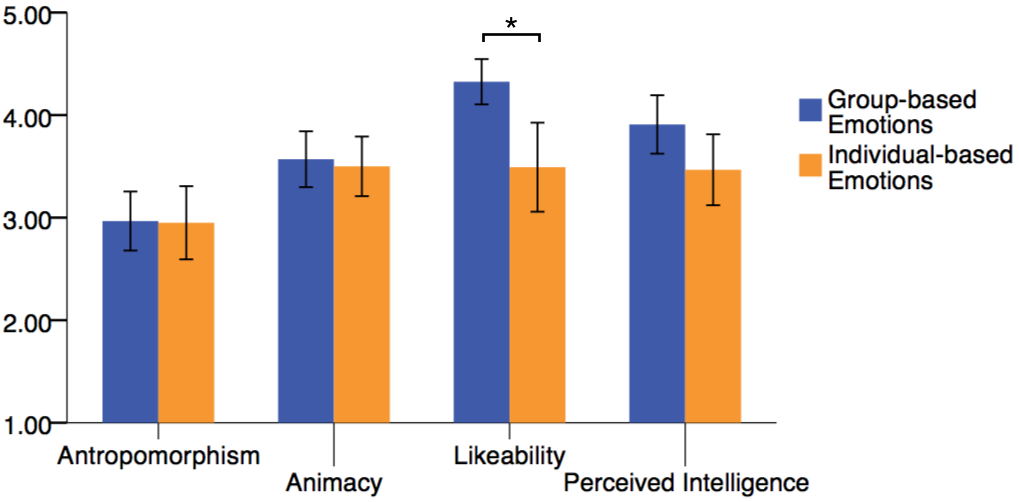
\includegraphics[width=0.7\columnwidth]{images/gbe/godspeed2.png}
    \caption{Averages of Godspeed's dimensions attributed to each robot. (*$p<0.05$)}
    \label{fig:godspeed}
\end{figure}

Additionally, a Spearman's rank-order correlation was run to determine the relationship between Group Identification and the four measured dimensions of the Godspeed Questionnaire. There was a strong, positive, and statistically significant correlations between Group Identification and Anthropomorphism ($r_s=0.529$,  $p<0.01$), Animacy ($r_s=0.318$, $p=0.03$), Likeability ($r_s=0.606$, $p<0.01$), and Perceived Intelligence ($r_s=0.595$, $p<0.01$).

\subsubsection{Group Trust}
A reliability analysis was carried out on the Group Trust scale comprising 7 items, respectively. Cronbach's alpha of 0.74 indicates a high level of internal consistency for this scale with this specific sample.

To check whether the portrayal of individual or group-based emotions was influencing the group trust, we compared the Group Trust levels of each human-robot team. Results showed a statistically significant difference of Group Trust ($U=148, p<0.01, r=0.417$). Partners of the robot with group-based emotions reported significantly higher levels of Group Trust ($M=5.45\pm0.16$) than participants partnering the robot with individual-based emotions ($M=4.62\pm0.20$), see Figure~\ref{fig:group-measures}.

Additionally, a Spearman's rank-order correlation was run to determine the relationship between Group Trust and the number of points of the team. Again, there was no significant correlation between the Group Trust and the number of points ($r_s=0.158$, $p=0.28$).

\section{Discussion}
\label{sec:study4-discussion}
Overall, the following conclusions can be drawn from the obtained results. \textbf{H1} predicted a stronger Group Identification with a robotic partner that expresses group-based emotions. Indeed, the expression of group-based emotions lead to higher levels of Group Identification. This result seem to be coherent with previous findings from the social psychology, where group-based emotions are an antecedent of Group Identification \cite{kessler2005group}.

Our results also partially support \textbf{H2}, which predicted a more positive perception of a robotic partner that expresses group-based emotions. Although participants perceived both robots similarly in terms of Anthropomorphism, Animacy, and Perceived Intelligence, they rated the robotic partner that expresses group-based emotions with significantly higher levels of Likeability. Our expectation was in-line with previous findings \cite{kuchenbrandt2013robot,haring2014would}, where the perceived group identity of a robot had a significant impact on how the robot is perceived. However, their manipulation of group identity referred to the extremes of belonging to the in-group or the out-group, stressing a stronger difference of Group Identification when compared to our setting. Therefore, even with a statistically significant difference of the Group Identification (H1), it was not prominent enough to elicit differences on the Anthropomorphism, Animacy, and Perceived Intelligence. Nevertheless, tendencies can be inferred in both Figure~\ref{fig:godspeed} and in the positive and significant correlations between the level of Group Identification and the measured dimensions of the Godspeed Questionnaire.

According to \textbf{H3}, we expected a higher degree of Group Trust with a robotic partner that has group-based emotions. This was confirmed as participants that were in the team of the robot that expresses group-based emotions attributed a higher level of trust towards the team. We believe this result is relevant for the emerging field of Human-Robot Teams, as trust constitutes one the most important constructs to support effective interaction and cooperation \cite{hancock2011meta}. Furthermore, trust and social identity have been postulated as antecedents of positive team performance \cite{allen2004exploring}.


\section{Concluding Remarks}
\label{sec:conclusind-remarks}
As human-robot groups become more prevalent, it is important to explore new ways of improving their interactions and creating effective collaborations. Therefore, this work provides a first exploration of group-based emotions in social robotic partners and tries to understand their impact on human-robot teams. The contributions are two fold. First, a model for generating group-based emotions on social robots is proposed. This model enabled the development of two distinct robotic characters that express either individual or group-based emotions. Second, it also contributes with a user study, where two fully autonomous robots formed two human-robot teams to play a competitive card game. We compared participants' perceptions, Group Identification, and Group Trust towards their robotic partners. The results show that the expression of group-based emotions by a social robotic partner led participants to rate it as more likeable, to trust it more as a team member and also to identify a stronger social group. Overall, group-based emotions were able to emphasise important aspects of the human-robot collaboration, as trust and group identification, revealing a promising role on the design of social robotic team partners.

One limitation of our study is related with the \textit{Sueca} scenario, as the generation of emotions is strongly related to the game itself. On the one hand, it is a very natural scenario for the interaction of autonomous robots with two people. On the other hand, it may result in an unbalanced number of positive emotions when compared to negative emotions in each game. As future work, it is important to explore scenarios where more negative events also occur. Additionally, the study reported here only analysed mixed human-robot teams of two. In the future, it would be important to analyse the effects of group-based emotions in larger teams as well. Finally, the fact that the robots used different wordings in their utterances could have generated a potential confound. For this reason, it would be interesting to analyse the effect of group-based emotions in a scenario with no use of verbal dialogue.

Our final argument is that social emotions such as shame or pride, which go beyond more basic emotions \cite{ekman1987universals}, should be given more attention in the creation of social robots, particularly in human-robot teams. The work presented here takes a step in this direction as it employs a more rich emotional model enabling social robots to autonomously produce more diverse emotional behaviour.
\chapter{Perception of the Communication Network}
\label{chapter:future-work}

The current chapter proposes an approach to achieve the last research goal of this ongoing dissertation ---\textit{develop computational mechanisms for the robotic teammate to autonomously perceive the structural cohesion of the team}. In order to explore structural cohesion, we plan to analyse the flow of the communication between team members. We aim to examine the following research questions:
\begin{itemize}
    \item Can we detect the communication network over time, i.e. who interacts with whom, using verbal and/or non-verbal cues?
    \item Are the features of this network, e.g. centrality of each member, correlated with subjective group measures? Can those features predict any subjective group measures, e.g. group identification?
    \item Can the robotic agent accurately infer the communication network in runtime?
    \item How can the robotic agent adapt its behaviour upon perceiving the communication network of its team?
\end{itemize}

In order to address these questions, we will create a new scenario that can increase the amount of interaction among team members compared to our previous scenarios of Sueca and For The Record (Section~\ref{sec:scenario}). Furthermore, we are considering a sequence of three user studies. The first one aims at collecting data from human participants playing this collaborative game in order to later develop the behaviours of a robotic teammate that will play the same game (Section~\ref{sec:fw-study1}). In the second user study, human participants will play together with the robot and the data collection will allow us to analyse communication patterns of the team (Section~\ref{sec:fw-study2}). Finally, the third user study will explore adaptive mechanisms on the behaviours of the robot and their impact on the communication network of the team (Section~\ref{sec:fw-study3}).

\section{For The Planet - Collaborative Game Scenario}
\label{sec:scenario}
The scenario is a collaborative game called For The Planet. It can be considered a new and improved version of the previous For The Record\footnote{\url{http://gaips.tagus.ist.utl.pt/~fcorreia/AAMAS19-FTR-demo.mp4}}, which was used in the experiment detailed in Chapter~\ref{chapter:pro-sociality}.

Generally, the game can be played by $N$ players and takes $R$ rounds. During each round, players face a decision of allocating $P$ points among two distinct abilities in the game. These abilities map either the degree of altruistic cooperation for the team, or the degree of individual income they can selfishly collect. In the end of the $R$ rounds, an objective measure of cooperation can be calculated for each player according to the sum of points he allocated in favour of the team.

There are two important distinctions between For The Planet and For The Record. The metaphor of the first game is related to the environment and climate change policies, while the latter has musical theme with purely entertaining purposes. We believe that the current concerns and discussions on the topic of climate change will engage people to interact more with each other while playing For The Planet. The second distinction is the non-binary choice between cooperating and defecting, previously imposed in For The Record. In other words, For The Planet allows players to choose the level of cooperation between a defined range of integers.

A completely new feature that was introduced into For The Planet (i.e., a feature that For The Record did not contain) is a free discussion period before players have to decide the allocation of their points. This free discussion period constitutes a face-to-face communication phase where, although players have no rules, they are expected to negotiate or persuade others of what to do next or comment their previous decisions. 

\section{Study 1 - Data Collection of Human Participants}
\label{sec:fw-study1}
The main goal of this first user study is to collect and analyse the behaviours that occur during the free discussion periods, which were not 
included in our previous version of the game. The development of behaviours for the robot in those particular situations can be hard to design without analysing first how do humans perform those negotiations. Therefore, we believe that creating those behaviours based on how humans communicate in those situations is a suitable approach.

A secondary goal of this study is to test and pilot the future setup that will accommodate the robotic player. Moreover, we plan to collect subjective perceptions of the group and of each individual teammate to test the reliability of the intended scales on this scenario.

\subsection{Participants}
Each session will have 3 players ---2 human participants and 1 confederate. The confederate will play the game according to a script and will ensure the discussion will be focused on game-related matters. We aim at collecting a small sample of 3 or 4 groups of adults (6 or 8 participants), outside the university campus and controlling for their mutual acquaintance.

\subsection{Materials}
The materials include: 1 tablet to play the game; 3 cameras that should be placed in front of each participant; and 3 lapel microphones. In terms of subjective scales for a final survey, we will use: group identification\cite{leach2008group}; group trust\cite{allen2004exploring}; group cohesiveness\cite{hoegl2001teamwork}; group rapport\cite{lafrance1979nonverbal}; perception of emergent leaders; perception of conflict.

\subsection{Procedure}
Participants will start watching the researcher playing a training game (according to a script), and they are allowed to ask questions in order to understand the rules of the game. Then, they play the game together and they finish the experiment with a final questionnaire.

%\subsection{Analysis}
%Overall, this user study will serve as a pilot of the game itself, the setup and the measurements. We would like to understand the variability of interactions that can emerge and how dependent those interactions are on the previous actions in the game. In particular, a current concern is if participants will discuss anything after everyone have cooperated with the team. In other words, we believe the degree of discussion is negatively correlated the cooperation rate in the previous rounds. If that is the case, future studies should consider the usage of confederates that assure the presence of non-cooperative behaviours, for instance.

%Regarding the development of behaviours for the robotic teammate, we would like to emphasise that we will carefully choose more neutral interactions (i.e., non-conflicting interactions). Although we acknowledge that the free discussion will allow for emergent leaders trying to persuade others, this is an important consideration to analyse participants' verbal and non-verbal behaviours.

\section{Study 2 - Data Collection of Human-Robot Teams}
\label{sec:fw-study2}
The second user study will be a follow-up of the first one. The idea is to script the verbal and non-verbal behaviours of the robot according to the interactions among humans from the previous study. The goal of study 2 is to collect data of human participants partnering with the robot.

\subsection{Participants}
Each session will have 2 human participants that will partner with the robotic teammate. We aim at collecting at least 30 groups of adults (60 participants), outside the university campus and controlling for their mutual acquaintance.

\subsection{Materials}
The materials include: 1 robot; 1 tablet to play the game; 2 cameras that should be placed in front of each participant; and 2 lapel microphones. In terms of subjective scales for a final survey, we will use: group identification\cite{leach2008group}; group trust\cite{allen2004exploring}; group cohesiveness\cite{hoegl2001teamwork}; group rapport\cite{lafrance1979nonverbal}; perception of emergent leaders; perception of conflict.

\subsection{Procedure}
Participants will start watching the researcher playing a training game (according to a script), and they are allowed to ask questions in order to understand the rules of the game. Then, they play the game with robot and they finish the experiment with a final questionnaire.

\subsection{Analysis}
The main analysis will use techniques from the Social Network Analysis (SNA) in order to derive the communication network of each team based on the speech acts between players during the game. In particular, we are currently interested in assessing the degree of centrality of each member. Additionally, we will perform a correlation analysis between the objective measures extracted from the communication network and the subjective measures assessed in the final survey. If we find strong and significant correlations, we will also try to create offline predictive models of the subjective measures using machine learning techniques.


\section{Study 3 - Exploring adaptive behaviours}
\label{sec:fw-study3}
In the third study, we aim at exploring new adaptive mechanisms to decide the behaviours of the robotic teammate. The idea is to infer the communication network in run-time (i.e., during the interaction) and intervene to modify that network. For instance, previous findings reported the satisfaction and closeness of a team can be hindered by the presence of members with high levels of centrality \cite{shaw1964communication}. A possible mechanism to cope with such issues could be to elicit interactions between members with low levels of centrality. The particular design of this user study is still a work in progress as it depends on the of the previous stages.


%\section{Follow-up Avenues}
%Succeeding in the previous tasks constitutes a significant step forward on the collaboration between humans and robots in small groups. Nevertheless, there are at least two interesting avenues to further explore: (1) how does the communication network change as the robotic teammate changes its actions in the game or its social behaviours; (2) how does the communication network change as the number of robots on the team increases.
%!TEX root = ../dissertation.tex

\chapter{Conclusion and Plan of Work}
\label{chapter:conclusion}

The current document reports an on-going dissertation on the topic of robotic teammates. In particular, this thesis explores the following research problem:

%reinforce why cohesion

\begin{indented}
How can we endow a social robot with the ability to improve the cohesive alliance in a team setting with humans?
\end{indented}

Our approach to address this problem consists of exploring two research goals. One of them is focused on investigating how human-robot teams are established, in particular analysing the perspective of human teammates on how should social robots integrate these teams. It involves the understanding of how people perceive robotic teammates, what people expect from them, or even what attitudes and predispositions people have towards them. Additionally, this research goal raises interesting challenges related to methodological aspects of analysing group interactions. From the careful selection of the group measures, to the adequate design of experiments, or even the correct statistical analysis of individual- and group-level factors.

The second research goal, on the other hand, is focused on the perspective of the social robot and what computational mechanisms it can apply in order to increase the effectiveness of the team. Such goal may also involve several challenges from the autonomous decision-making process, to its perceptive capabilities, or even to the authoring of its social behaviours. The current contributions to this research goal explore novel approaches for the decision-making of robotic teammates.

Overall, 

Finally, we would like to highlight the following publications that are explicitly linked to the goals of this dissertation:
\begin{itemize}
    \item Correia, F., Petisca, S., Alves-Oliveira, P., Ribeiro, T., Melo, F. S., \& Paiva, A. (2017, July). Groups of humans and robots: Understanding membership preferences and team formation. In Robotics: Science and Systems (RSS).
    \item Correia, F., Petisca, S., Alves-Oliveira, P., Ribeiro, T., Melo, F. S., \& Paiva, A. (2019). ``I Choose... YOU!'' Membership preferences in human–robot teams. Autonomous Robots, 43(2), 359-373.
    \item Correia, F., Mascarenhas, S. F., Gomes, S., Arriaga, P., Leite, I., Prada, R., Melo, F. S. \& Paiva, A. (2019, March). Exploring prosociality in human-robot teams. In 2019 14th ACM/IEEE International Conference on Human-Robot Interaction (HRI) (pp. 143-151). IEEE.
    \item Correia, F., Mascarenhas, S., Prada, R., Melo, F. S., \& Paiva, A. (2018, February). Group-based emotions in teams of humans and robots. In Proceedings of the 2018 ACM/IEEE International Conference on Human-Robot Interaction (pp. 261-269). ACM.
    \item Correia, F., Melo, F. S., \& Paiva, A. (2019, March). Group Intelligence on Social Robots. In 2019 14th ACM/IEEE International Conference on Human-Robot Interaction (HRI Pioneers Workshop) (pp. 703-705). IEEE.
\end{itemize}


Furthermore, beyond the focus of this dissertation on establishing cohesive alliances with robotic teammates, we also contributed to the HRI field with additional publications. The following list contains only the publications involving group interactions, which are related to the scope of this dissertation:
\begin{itemize}
    \item Oliveira, R., Arriaga, P., Alves-Oliveira, P., Correia, F., Petisca, S., \& Paiva, A. (2018, February). Friends or foes?: Socioemotional support and gaze behaviors in mixed groups of humans and robots. In Proceedings of the 2018 ACM/IEEE International Conference on Human-Robot Interaction (pp. 279-288). ACM.
    \item Oliveira, R., Arriaga, P., Correia, F. \& Paiva. A. (2019, March) Looking Beyond Collaboration: Socioemotional Positive, Negative and Task-oriented Behaviors in Human-Robot Group Interactions. In International Journal of Social Robotics
    \item Oliveira, R., Arriaga, P., Correia, F., \& Paiva, A. (2019, March). The Stereotype Content Model Applied to Human-Robot Interactions in Groups. In 2019 14th ACM/IEEE International Conference on Human-Robot Interaction (HRI) (pp. 123-132). IEEE.
    \item Correia, F., Chandra, S., Mascarenhas, S., Charles-Nicolas, J., Gally, J., Lopes, D., Santos, F. P., Santos, F. C., Melo, F. S. \& Paiva, A. (2019, October). Walk the Talk! Exploring (Mis)Alignment of Words and Deeds by Robotic Teammates in a Public Goods Game. In 28th IEEE international symposium on robot and human interactive communication (RO-MAN). IEEE.
    \item Correia, F., Mascarenhas, S., Gomes, S., Melo, F. S., \& Paiva, A. The Dark Side of Embodiment - Teaming Up With Robots VS Disembodied Agents. (2020, SUBMITTED).
\end{itemize}


\section{Work Plan}
%Additionally, the future work we have proposed in Chapter~\ref{chapter:future-work} also aims at contributing to this research goal by enhancing the perceptive capabilities of robotic teammates.
According to the proposed work detailed in Chapter~\ref{chapter:future-work}, we are currently considering a sequence of three user studies. \textit{Study 1} aims at collecting data from human participants playing a collaborative game and negotiating with team members in order to later develop the behaviours of a robotic teammate that will play the same game. In \textit{Study 2}, human participants will play together with a robot and the data collection will allow us to analyse communication patterns of the team when there is a robotic partner. Finally, the \textit{Study 3} will explore adaptive mechanisms on the behaviours of the robot and their impact on the communication network of the team.


\begin{table}[h]
\centering
\caption{Work plan for the proposed work}
\begin{tabular}{|r|l|} 
\hline
\textbf{Winter 2019} & Study 1            \\ 
\hline
\textbf{Spring 2020} & Visit another lab  \\ 
\hline
\textbf{Summer 2020} & Study 2            \\ 
\hline
\textbf{Fall 2020}   & Study 3            \\ 
\hline
\textbf{Winter 2020} & Writing thesis     \\
\hline
\end{tabular}
\end{table}

\section*{\centering*}
This dissertation proposes two research goals that address the research problem by two different perspectives. These research goals hold complementary and, at a certain extent, interdependent challenges that reflect the interdisciplinarity of the HRI field. Overall, we believe its contributions strongly support and enhance research on group interactions with robotic teammates.

\bibliographystyle{ieeetr}
\addcontentsline{toc}{chapter}{Bibliography}
\bibliography{bibliography/dissertation}

% Appendix
%\appendix
%%!TEX root = ../dissertation.tex

% Appendix chapters entry point
% Include the chapters below

%!TEX root = ../dissertation.tex

%\chapter{Additional Publications}
%\label{appendix:additional-publications}


% Glossary and Acronym List
\if\includeGlossary 1
\printglossary
\fi

\end{document}